\documentclass[11pt]{article}

    \usepackage[breakable]{tcolorbox}
    \usepackage{parskip} % Stop auto-indenting (to mimic markdown behaviour)
    
    \usepackage{iftex}
    \ifPDFTeX
    	\usepackage[T1]{fontenc}
    	\usepackage{mathpazo}
    \else
    	\usepackage{fontspec}
    \fi

    % Basic figure setup, for now with no caption control since it's done
    % automatically by Pandoc (which extracts ![](path) syntax from Markdown).
    \usepackage{graphicx}
    % Maintain compatibility with old templates. Remove in nbconvert 6.0
    \let\Oldincludegraphics\includegraphics
    % Ensure that by default, figures have no caption (until we provide a
    % proper Figure object with a Caption API and a way to capture that
    % in the conversion process - todo).
    \usepackage{caption}
    \DeclareCaptionFormat{nocaption}{}
    \captionsetup{format=nocaption,aboveskip=0pt,belowskip=0pt}

    \usepackage[Export]{adjustbox} % Used to constrain images to a maximum size
    \adjustboxset{max size={0.9\linewidth}{0.9\paperheight}}
    \usepackage{float}
    \floatplacement{figure}{H} % forces figures to be placed at the correct location
    \usepackage{xcolor} % Allow colors to be defined
    \usepackage{enumerate} % Needed for markdown enumerations to work
    \usepackage{geometry} % Used to adjust the document margins
    \usepackage{amsmath} % Equations
    \usepackage{amssymb} % Equations
    \usepackage{textcomp} % defines textquotesingle
    % Hack from http://tex.stackexchange.com/a/47451/13684:
    \AtBeginDocument{%
        \def\PYZsq{\textquotesingle}% Upright quotes in Pygmentized code
    }
    \usepackage{upquote} % Upright quotes for verbatim code
    \usepackage{eurosym} % defines \euro
    \usepackage[mathletters]{ucs} % Extended unicode (utf-8) support
    \usepackage{fancyvrb} % verbatim replacement that allows latex
    \usepackage{grffile} % extends the file name processing of package graphics 
                         % to support a larger range
    \makeatletter % fix for grffile with XeLaTeX
    \def\Gread@@xetex#1{%
      \IfFileExists{"\Gin@base".bb}%
      {\Gread@eps{\Gin@base.bb}}%
      {\Gread@@xetex@aux#1}%
    }
    \makeatother

    % The hyperref package gives us a pdf with properly built
    % internal navigation ('pdf bookmarks' for the table of contents,
    % internal cross-reference links, web links for URLs, etc.)
    \usepackage{hyperref}
    % The default LaTeX title has an obnoxious amount of whitespace. By default,
    % titling removes some of it. It also provides customization options.
    \usepackage{titling}
    \usepackage{longtable} % longtable support required by pandoc >1.10
    \usepackage{booktabs}  % table support for pandoc > 1.12.2
    \usepackage[inline]{enumitem} % IRkernel/repr support (it uses the enumerate* environment)
    \usepackage[normalem]{ulem} % ulem is needed to support strikethroughs (\sout)
                                % normalem makes italics be italics, not underlines
    \usepackage{mathrsfs}
    

    
    % Colors for the hyperref package
    \definecolor{urlcolor}{rgb}{0,.145,.698}
    \definecolor{linkcolor}{rgb}{.71,0.21,0.01}
    \definecolor{citecolor}{rgb}{.12,.54,.11}

    % ANSI colors
    \definecolor{ansi-black}{HTML}{3E424D}
    \definecolor{ansi-black-intense}{HTML}{282C36}
    \definecolor{ansi-red}{HTML}{E75C58}
    \definecolor{ansi-red-intense}{HTML}{B22B31}
    \definecolor{ansi-green}{HTML}{00A250}
    \definecolor{ansi-green-intense}{HTML}{007427}
    \definecolor{ansi-yellow}{HTML}{DDB62B}
    \definecolor{ansi-yellow-intense}{HTML}{B27D12}
    \definecolor{ansi-blue}{HTML}{208FFB}
    \definecolor{ansi-blue-intense}{HTML}{0065CA}
    \definecolor{ansi-magenta}{HTML}{D160C4}
    \definecolor{ansi-magenta-intense}{HTML}{A03196}
    \definecolor{ansi-cyan}{HTML}{60C6C8}
    \definecolor{ansi-cyan-intense}{HTML}{258F8F}
    \definecolor{ansi-white}{HTML}{C5C1B4}
    \definecolor{ansi-white-intense}{HTML}{A1A6B2}
    \definecolor{ansi-default-inverse-fg}{HTML}{FFFFFF}
    \definecolor{ansi-default-inverse-bg}{HTML}{000000}

    % commands and environments needed by pandoc snippets
    % extracted from the output of `pandoc -s`
    \providecommand{\tightlist}{%
      \setlength{\itemsep}{0pt}\setlength{\parskip}{0pt}}
    \DefineVerbatimEnvironment{Highlighting}{Verbatim}{commandchars=\\\{\}}
    % Add ',fontsize=\small' for more characters per line
    \newenvironment{Shaded}{}{}
    \newcommand{\KeywordTok}[1]{\textcolor[rgb]{0.00,0.44,0.13}{\textbf{{#1}}}}
    \newcommand{\DataTypeTok}[1]{\textcolor[rgb]{0.56,0.13,0.00}{{#1}}}
    \newcommand{\DecValTok}[1]{\textcolor[rgb]{0.25,0.63,0.44}{{#1}}}
    \newcommand{\BaseNTok}[1]{\textcolor[rgb]{0.25,0.63,0.44}{{#1}}}
    \newcommand{\FloatTok}[1]{\textcolor[rgb]{0.25,0.63,0.44}{{#1}}}
    \newcommand{\CharTok}[1]{\textcolor[rgb]{0.25,0.44,0.63}{{#1}}}
    \newcommand{\StringTok}[1]{\textcolor[rgb]{0.25,0.44,0.63}{{#1}}}
    \newcommand{\CommentTok}[1]{\textcolor[rgb]{0.38,0.63,0.69}{\textit{{#1}}}}
    \newcommand{\OtherTok}[1]{\textcolor[rgb]{0.00,0.44,0.13}{{#1}}}
    \newcommand{\AlertTok}[1]{\textcolor[rgb]{1.00,0.00,0.00}{\textbf{{#1}}}}
    \newcommand{\FunctionTok}[1]{\textcolor[rgb]{0.02,0.16,0.49}{{#1}}}
    \newcommand{\RegionMarkerTok}[1]{{#1}}
    \newcommand{\ErrorTok}[1]{\textcolor[rgb]{1.00,0.00,0.00}{\textbf{{#1}}}}
    \newcommand{\NormalTok}[1]{{#1}}
    
    % Additional commands for more recent versions of Pandoc
    \newcommand{\ConstantTok}[1]{\textcolor[rgb]{0.53,0.00,0.00}{{#1}}}
    \newcommand{\SpecialCharTok}[1]{\textcolor[rgb]{0.25,0.44,0.63}{{#1}}}
    \newcommand{\VerbatimStringTok}[1]{\textcolor[rgb]{0.25,0.44,0.63}{{#1}}}
    \newcommand{\SpecialStringTok}[1]{\textcolor[rgb]{0.73,0.40,0.53}{{#1}}}
    \newcommand{\ImportTok}[1]{{#1}}
    \newcommand{\DocumentationTok}[1]{\textcolor[rgb]{0.73,0.13,0.13}{\textit{{#1}}}}
    \newcommand{\AnnotationTok}[1]{\textcolor[rgb]{0.38,0.63,0.69}{\textbf{\textit{{#1}}}}}
    \newcommand{\CommentVarTok}[1]{\textcolor[rgb]{0.38,0.63,0.69}{\textbf{\textit{{#1}}}}}
    \newcommand{\VariableTok}[1]{\textcolor[rgb]{0.10,0.09,0.49}{{#1}}}
    \newcommand{\ControlFlowTok}[1]{\textcolor[rgb]{0.00,0.44,0.13}{\textbf{{#1}}}}
    \newcommand{\OperatorTok}[1]{\textcolor[rgb]{0.40,0.40,0.40}{{#1}}}
    \newcommand{\BuiltInTok}[1]{{#1}}
    \newcommand{\ExtensionTok}[1]{{#1}}
    \newcommand{\PreprocessorTok}[1]{\textcolor[rgb]{0.74,0.48,0.00}{{#1}}}
    \newcommand{\AttributeTok}[1]{\textcolor[rgb]{0.49,0.56,0.16}{{#1}}}
    \newcommand{\InformationTok}[1]{\textcolor[rgb]{0.38,0.63,0.69}{\textbf{\textit{{#1}}}}}
    \newcommand{\WarningTok}[1]{\textcolor[rgb]{0.38,0.63,0.69}{\textbf{\textit{{#1}}}}}
    
    
    % Define a nice break command that doesn't care if a line doesn't already
    % exist.
    \def\br{\hspace*{\fill} \\* }
    % Math Jax compatibility definitions
    \def\gt{>}
    \def\lt{<}
    \let\Oldtex\TeX
    \let\Oldlatex\LaTeX
    \renewcommand{\TeX}{\textrm{\Oldtex}}
    \renewcommand{\LaTeX}{\textrm{\Oldlatex}}
    % Document parameters
    % Document title
    \title{SimRisk: A simulation-based covid-19 risk estimator}
    
    
    
    \author{Ronald L. Rivest}
    
    
    
% Pygments definitions
\makeatletter
\def\PY@reset{\let\PY@it=\relax \let\PY@bf=\relax%
    \let\PY@ul=\relax \let\PY@tc=\relax%
    \let\PY@bc=\relax \let\PY@ff=\relax}
\def\PY@tok#1{\csname PY@tok@#1\endcsname}
\def\PY@toks#1+{\ifx\relax#1\empty\else%
    \PY@tok{#1}\expandafter\PY@toks\fi}
\def\PY@do#1{\PY@bc{\PY@tc{\PY@ul{%
    \PY@it{\PY@bf{\PY@ff{#1}}}}}}}
\def\PY#1#2{\PY@reset\PY@toks#1+\relax+\PY@do{#2}}

\expandafter\def\csname PY@tok@w\endcsname{\def\PY@tc##1{\textcolor[rgb]{0.73,0.73,0.73}{##1}}}
\expandafter\def\csname PY@tok@c\endcsname{\let\PY@it=\textit\def\PY@tc##1{\textcolor[rgb]{0.25,0.50,0.50}{##1}}}
\expandafter\def\csname PY@tok@cp\endcsname{\def\PY@tc##1{\textcolor[rgb]{0.74,0.48,0.00}{##1}}}
\expandafter\def\csname PY@tok@k\endcsname{\let\PY@bf=\textbf\def\PY@tc##1{\textcolor[rgb]{0.00,0.50,0.00}{##1}}}
\expandafter\def\csname PY@tok@kp\endcsname{\def\PY@tc##1{\textcolor[rgb]{0.00,0.50,0.00}{##1}}}
\expandafter\def\csname PY@tok@kt\endcsname{\def\PY@tc##1{\textcolor[rgb]{0.69,0.00,0.25}{##1}}}
\expandafter\def\csname PY@tok@o\endcsname{\def\PY@tc##1{\textcolor[rgb]{0.40,0.40,0.40}{##1}}}
\expandafter\def\csname PY@tok@ow\endcsname{\let\PY@bf=\textbf\def\PY@tc##1{\textcolor[rgb]{0.67,0.13,1.00}{##1}}}
\expandafter\def\csname PY@tok@nb\endcsname{\def\PY@tc##1{\textcolor[rgb]{0.00,0.50,0.00}{##1}}}
\expandafter\def\csname PY@tok@nf\endcsname{\def\PY@tc##1{\textcolor[rgb]{0.00,0.00,1.00}{##1}}}
\expandafter\def\csname PY@tok@nc\endcsname{\let\PY@bf=\textbf\def\PY@tc##1{\textcolor[rgb]{0.00,0.00,1.00}{##1}}}
\expandafter\def\csname PY@tok@nn\endcsname{\let\PY@bf=\textbf\def\PY@tc##1{\textcolor[rgb]{0.00,0.00,1.00}{##1}}}
\expandafter\def\csname PY@tok@ne\endcsname{\let\PY@bf=\textbf\def\PY@tc##1{\textcolor[rgb]{0.82,0.25,0.23}{##1}}}
\expandafter\def\csname PY@tok@nv\endcsname{\def\PY@tc##1{\textcolor[rgb]{0.10,0.09,0.49}{##1}}}
\expandafter\def\csname PY@tok@no\endcsname{\def\PY@tc##1{\textcolor[rgb]{0.53,0.00,0.00}{##1}}}
\expandafter\def\csname PY@tok@nl\endcsname{\def\PY@tc##1{\textcolor[rgb]{0.63,0.63,0.00}{##1}}}
\expandafter\def\csname PY@tok@ni\endcsname{\let\PY@bf=\textbf\def\PY@tc##1{\textcolor[rgb]{0.60,0.60,0.60}{##1}}}
\expandafter\def\csname PY@tok@na\endcsname{\def\PY@tc##1{\textcolor[rgb]{0.49,0.56,0.16}{##1}}}
\expandafter\def\csname PY@tok@nt\endcsname{\let\PY@bf=\textbf\def\PY@tc##1{\textcolor[rgb]{0.00,0.50,0.00}{##1}}}
\expandafter\def\csname PY@tok@nd\endcsname{\def\PY@tc##1{\textcolor[rgb]{0.67,0.13,1.00}{##1}}}
\expandafter\def\csname PY@tok@s\endcsname{\def\PY@tc##1{\textcolor[rgb]{0.73,0.13,0.13}{##1}}}
\expandafter\def\csname PY@tok@sd\endcsname{\let\PY@it=\textit\def\PY@tc##1{\textcolor[rgb]{0.73,0.13,0.13}{##1}}}
\expandafter\def\csname PY@tok@si\endcsname{\let\PY@bf=\textbf\def\PY@tc##1{\textcolor[rgb]{0.73,0.40,0.53}{##1}}}
\expandafter\def\csname PY@tok@se\endcsname{\let\PY@bf=\textbf\def\PY@tc##1{\textcolor[rgb]{0.73,0.40,0.13}{##1}}}
\expandafter\def\csname PY@tok@sr\endcsname{\def\PY@tc##1{\textcolor[rgb]{0.73,0.40,0.53}{##1}}}
\expandafter\def\csname PY@tok@ss\endcsname{\def\PY@tc##1{\textcolor[rgb]{0.10,0.09,0.49}{##1}}}
\expandafter\def\csname PY@tok@sx\endcsname{\def\PY@tc##1{\textcolor[rgb]{0.00,0.50,0.00}{##1}}}
\expandafter\def\csname PY@tok@m\endcsname{\def\PY@tc##1{\textcolor[rgb]{0.40,0.40,0.40}{##1}}}
\expandafter\def\csname PY@tok@gh\endcsname{\let\PY@bf=\textbf\def\PY@tc##1{\textcolor[rgb]{0.00,0.00,0.50}{##1}}}
\expandafter\def\csname PY@tok@gu\endcsname{\let\PY@bf=\textbf\def\PY@tc##1{\textcolor[rgb]{0.50,0.00,0.50}{##1}}}
\expandafter\def\csname PY@tok@gd\endcsname{\def\PY@tc##1{\textcolor[rgb]{0.63,0.00,0.00}{##1}}}
\expandafter\def\csname PY@tok@gi\endcsname{\def\PY@tc##1{\textcolor[rgb]{0.00,0.63,0.00}{##1}}}
\expandafter\def\csname PY@tok@gr\endcsname{\def\PY@tc##1{\textcolor[rgb]{1.00,0.00,0.00}{##1}}}
\expandafter\def\csname PY@tok@ge\endcsname{\let\PY@it=\textit}
\expandafter\def\csname PY@tok@gs\endcsname{\let\PY@bf=\textbf}
\expandafter\def\csname PY@tok@gp\endcsname{\let\PY@bf=\textbf\def\PY@tc##1{\textcolor[rgb]{0.00,0.00,0.50}{##1}}}
\expandafter\def\csname PY@tok@go\endcsname{\def\PY@tc##1{\textcolor[rgb]{0.53,0.53,0.53}{##1}}}
\expandafter\def\csname PY@tok@gt\endcsname{\def\PY@tc##1{\textcolor[rgb]{0.00,0.27,0.87}{##1}}}
\expandafter\def\csname PY@tok@err\endcsname{\def\PY@bc##1{\setlength{\fboxsep}{0pt}\fcolorbox[rgb]{1.00,0.00,0.00}{1,1,1}{\strut ##1}}}
\expandafter\def\csname PY@tok@kc\endcsname{\let\PY@bf=\textbf\def\PY@tc##1{\textcolor[rgb]{0.00,0.50,0.00}{##1}}}
\expandafter\def\csname PY@tok@kd\endcsname{\let\PY@bf=\textbf\def\PY@tc##1{\textcolor[rgb]{0.00,0.50,0.00}{##1}}}
\expandafter\def\csname PY@tok@kn\endcsname{\let\PY@bf=\textbf\def\PY@tc##1{\textcolor[rgb]{0.00,0.50,0.00}{##1}}}
\expandafter\def\csname PY@tok@kr\endcsname{\let\PY@bf=\textbf\def\PY@tc##1{\textcolor[rgb]{0.00,0.50,0.00}{##1}}}
\expandafter\def\csname PY@tok@bp\endcsname{\def\PY@tc##1{\textcolor[rgb]{0.00,0.50,0.00}{##1}}}
\expandafter\def\csname PY@tok@fm\endcsname{\def\PY@tc##1{\textcolor[rgb]{0.00,0.00,1.00}{##1}}}
\expandafter\def\csname PY@tok@vc\endcsname{\def\PY@tc##1{\textcolor[rgb]{0.10,0.09,0.49}{##1}}}
\expandafter\def\csname PY@tok@vg\endcsname{\def\PY@tc##1{\textcolor[rgb]{0.10,0.09,0.49}{##1}}}
\expandafter\def\csname PY@tok@vi\endcsname{\def\PY@tc##1{\textcolor[rgb]{0.10,0.09,0.49}{##1}}}
\expandafter\def\csname PY@tok@vm\endcsname{\def\PY@tc##1{\textcolor[rgb]{0.10,0.09,0.49}{##1}}}
\expandafter\def\csname PY@tok@sa\endcsname{\def\PY@tc##1{\textcolor[rgb]{0.73,0.13,0.13}{##1}}}
\expandafter\def\csname PY@tok@sb\endcsname{\def\PY@tc##1{\textcolor[rgb]{0.73,0.13,0.13}{##1}}}
\expandafter\def\csname PY@tok@sc\endcsname{\def\PY@tc##1{\textcolor[rgb]{0.73,0.13,0.13}{##1}}}
\expandafter\def\csname PY@tok@dl\endcsname{\def\PY@tc##1{\textcolor[rgb]{0.73,0.13,0.13}{##1}}}
\expandafter\def\csname PY@tok@s2\endcsname{\def\PY@tc##1{\textcolor[rgb]{0.73,0.13,0.13}{##1}}}
\expandafter\def\csname PY@tok@sh\endcsname{\def\PY@tc##1{\textcolor[rgb]{0.73,0.13,0.13}{##1}}}
\expandafter\def\csname PY@tok@s1\endcsname{\def\PY@tc##1{\textcolor[rgb]{0.73,0.13,0.13}{##1}}}
\expandafter\def\csname PY@tok@mb\endcsname{\def\PY@tc##1{\textcolor[rgb]{0.40,0.40,0.40}{##1}}}
\expandafter\def\csname PY@tok@mf\endcsname{\def\PY@tc##1{\textcolor[rgb]{0.40,0.40,0.40}{##1}}}
\expandafter\def\csname PY@tok@mh\endcsname{\def\PY@tc##1{\textcolor[rgb]{0.40,0.40,0.40}{##1}}}
\expandafter\def\csname PY@tok@mi\endcsname{\def\PY@tc##1{\textcolor[rgb]{0.40,0.40,0.40}{##1}}}
\expandafter\def\csname PY@tok@il\endcsname{\def\PY@tc##1{\textcolor[rgb]{0.40,0.40,0.40}{##1}}}
\expandafter\def\csname PY@tok@mo\endcsname{\def\PY@tc##1{\textcolor[rgb]{0.40,0.40,0.40}{##1}}}
\expandafter\def\csname PY@tok@ch\endcsname{\let\PY@it=\textit\def\PY@tc##1{\textcolor[rgb]{0.25,0.50,0.50}{##1}}}
\expandafter\def\csname PY@tok@cm\endcsname{\let\PY@it=\textit\def\PY@tc##1{\textcolor[rgb]{0.25,0.50,0.50}{##1}}}
\expandafter\def\csname PY@tok@cpf\endcsname{\let\PY@it=\textit\def\PY@tc##1{\textcolor[rgb]{0.25,0.50,0.50}{##1}}}
\expandafter\def\csname PY@tok@c1\endcsname{\let\PY@it=\textit\def\PY@tc##1{\textcolor[rgb]{0.25,0.50,0.50}{##1}}}
\expandafter\def\csname PY@tok@cs\endcsname{\let\PY@it=\textit\def\PY@tc##1{\textcolor[rgb]{0.25,0.50,0.50}{##1}}}

\def\PYZbs{\char`\\}
\def\PYZus{\char`\_}
\def\PYZob{\char`\{}
\def\PYZcb{\char`\}}
\def\PYZca{\char`\^}
\def\PYZam{\char`\&}
\def\PYZlt{\char`\<}
\def\PYZgt{\char`\>}
\def\PYZsh{\char`\#}
\def\PYZpc{\char`\%}
\def\PYZdl{\char`\$}
\def\PYZhy{\char`\-}
\def\PYZsq{\char`\'}
\def\PYZdq{\char`\"}
\def\PYZti{\char`\~}
% for compatibility with earlier versions
\def\PYZat{@}
\def\PYZlb{[}
\def\PYZrb{]}
\makeatother


    % For linebreaks inside Verbatim environment from package fancyvrb. 
    \makeatletter
        \newbox\Wrappedcontinuationbox 
        \newbox\Wrappedvisiblespacebox 
        \newcommand*\Wrappedvisiblespace {\textcolor{red}{\textvisiblespace}} 
        \newcommand*\Wrappedcontinuationsymbol {\textcolor{red}{\llap{\tiny$\m@th\hookrightarrow$}}} 
        \newcommand*\Wrappedcontinuationindent {3ex } 
        \newcommand*\Wrappedafterbreak {\kern\Wrappedcontinuationindent\copy\Wrappedcontinuationbox} 
        % Take advantage of the already applied Pygments mark-up to insert 
        % potential linebreaks for TeX processing. 
        %        {, <, #, %, $, ' and ": go to next line. 
        %        _, }, ^, &, >, - and ~: stay at end of broken line. 
        % Use of \textquotesingle for straight quote. 
        \newcommand*\Wrappedbreaksatspecials {% 
            \def\PYGZus{\discretionary{\char`\_}{\Wrappedafterbreak}{\char`\_}}% 
            \def\PYGZob{\discretionary{}{\Wrappedafterbreak\char`\{}{\char`\{}}% 
            \def\PYGZcb{\discretionary{\char`\}}{\Wrappedafterbreak}{\char`\}}}% 
            \def\PYGZca{\discretionary{\char`\^}{\Wrappedafterbreak}{\char`\^}}% 
            \def\PYGZam{\discretionary{\char`\&}{\Wrappedafterbreak}{\char`\&}}% 
            \def\PYGZlt{\discretionary{}{\Wrappedafterbreak\char`\<}{\char`\<}}% 
            \def\PYGZgt{\discretionary{\char`\>}{\Wrappedafterbreak}{\char`\>}}% 
            \def\PYGZsh{\discretionary{}{\Wrappedafterbreak\char`\#}{\char`\#}}% 
            \def\PYGZpc{\discretionary{}{\Wrappedafterbreak\char`\%}{\char`\%}}% 
            \def\PYGZdl{\discretionary{}{\Wrappedafterbreak\char`\$}{\char`\$}}% 
            \def\PYGZhy{\discretionary{\char`\-}{\Wrappedafterbreak}{\char`\-}}% 
            \def\PYGZsq{\discretionary{}{\Wrappedafterbreak\textquotesingle}{\textquotesingle}}% 
            \def\PYGZdq{\discretionary{}{\Wrappedafterbreak\char`\"}{\char`\"}}% 
            \def\PYGZti{\discretionary{\char`\~}{\Wrappedafterbreak}{\char`\~}}% 
        } 
        % Some characters . , ; ? ! / are not pygmentized. 
        % This macro makes them "active" and they will insert potential linebreaks 
        \newcommand*\Wrappedbreaksatpunct {% 
            \lccode`\~`\.\lowercase{\def~}{\discretionary{\hbox{\char`\.}}{\Wrappedafterbreak}{\hbox{\char`\.}}}% 
            \lccode`\~`\,\lowercase{\def~}{\discretionary{\hbox{\char`\,}}{\Wrappedafterbreak}{\hbox{\char`\,}}}% 
            \lccode`\~`\;\lowercase{\def~}{\discretionary{\hbox{\char`\;}}{\Wrappedafterbreak}{\hbox{\char`\;}}}% 
            \lccode`\~`\:\lowercase{\def~}{\discretionary{\hbox{\char`\:}}{\Wrappedafterbreak}{\hbox{\char`\:}}}% 
            \lccode`\~`\?\lowercase{\def~}{\discretionary{\hbox{\char`\?}}{\Wrappedafterbreak}{\hbox{\char`\?}}}% 
            \lccode`\~`\!\lowercase{\def~}{\discretionary{\hbox{\char`\!}}{\Wrappedafterbreak}{\hbox{\char`\!}}}% 
            \lccode`\~`\/\lowercase{\def~}{\discretionary{\hbox{\char`\/}}{\Wrappedafterbreak}{\hbox{\char`\/}}}% 
            \catcode`\.\active
            \catcode`\,\active 
            \catcode`\;\active
            \catcode`\:\active
            \catcode`\?\active
            \catcode`\!\active
            \catcode`\/\active 
            \lccode`\~`\~ 	
        }
    \makeatother

    \let\OriginalVerbatim=\Verbatim
    \makeatletter
    \renewcommand{\Verbatim}[1][1]{%
        %\parskip\z@skip
        \sbox\Wrappedcontinuationbox {\Wrappedcontinuationsymbol}%
        \sbox\Wrappedvisiblespacebox {\FV@SetupFont\Wrappedvisiblespace}%
        \def\FancyVerbFormatLine ##1{\hsize\linewidth
            \vtop{\raggedright\hyphenpenalty\z@\exhyphenpenalty\z@
                \doublehyphendemerits\z@\finalhyphendemerits\z@
                \strut ##1\strut}%
        }%
        % If the linebreak is at a space, the latter will be displayed as visible
        % space at end of first line, and a continuation symbol starts next line.
        % Stretch/shrink are however usually zero for typewriter font.
        \def\FV@Space {%
            \nobreak\hskip\z@ plus\fontdimen3\font minus\fontdimen4\font
            \discretionary{\copy\Wrappedvisiblespacebox}{\Wrappedafterbreak}
            {\kern\fontdimen2\font}%
        }%
        
        % Allow breaks at special characters using \PYG... macros.
        \Wrappedbreaksatspecials
        % Breaks at punctuation characters . , ; ? ! and / need catcode=\active 	
        \OriginalVerbatim[#1,codes*=\Wrappedbreaksatpunct]%
    }
    \makeatother

    % Exact colors from NB
    \definecolor{incolor}{HTML}{303F9F}
    \definecolor{outcolor}{HTML}{D84315}
    \definecolor{cellborder}{HTML}{CFCFCF}
    \definecolor{cellbackground}{HTML}{F7F7F7}
    
    % prompt
    \makeatletter
    \newcommand{\boxspacing}{\kern\kvtcb@left@rule\kern\kvtcb@boxsep}
    \makeatother
    \newcommand{\prompt}[4]{
        \ttfamily\llap{{\color{#2}[#3]:\hspace{3pt}#4}}\vspace{-\baselineskip}
    }
    

    
    % Prevent overflowing lines due to hard-to-break entities
    \sloppy 
    % Setup hyperref package
    \hypersetup{
      breaklinks=true,  % so long urls are correctly broken across lines
      colorlinks=true,
      urlcolor=urlcolor,
      linkcolor=linkcolor,
      citecolor=citecolor,
      }
    % Slightly bigger margins than the latex defaults
    
    \geometry{verbose,tmargin=1in,bmargin=1in,lmargin=1in,rmargin=1in}
    
    

\begin{document}
    
    \maketitle
    
    

    
    \textbf{Abstract}

This note and Julia notebook presents a simulation-based method and
associated Julia software package for estimating covid-19 infection
risks.

Our approach differs from many covid-19 simulations, in that it is
\emph{small-scale}: it doesn't try to model an entire population, but
only a few individuals (from one to perhaps two dozen). The primary goal
is to estimate the probability that each individual is infected, based
on a history of their recent contacts and test results (as well as
certain assumptions and other information).

A simulation consists of many \emph{simulation runs}; we also call a
simulation run a \emph{scenario}. Each simulation run is based on the
provided history of contacts and test results, but may vary in the
pattern of how infection spreads among the individuals. Simulation runs
that give results inconsistent with provided test results are discarded.
The probability that an individual is infected at the end is estimated
as the fraction of remaining simulation runs in which that individual is
infected.

A simulation may also take into account: * whether individuals are
wearing \textbf{masks} (and if so, what type of mask) * the
\textbf{duration} of contacts (disease transmission is modeled in a
\textbf{dose-based} manner) * \textbf{multi-person contacts} (e.g.~for a
dinner) * the presence of one or more \textbf{anonymous individuals} in
a multi-person contact (e.g.~bus riders) * given probabilities for the
prevalence of the disease in the population, and the likelihood of
mask-wearing in the population, both used to model anonymous individuals
* different \textbf{types of tests} with differing probabilities for
detection and false alarms * many infected individuals are
\textbf{asymptomatic} * infected individuals progress through a series
of stages of the disease, * the \textbf{infectiousness} of an infected
individual may vary over time, * infected individuals typically recover
after a certain time (e.g.~14 days) * an infected individual, if
symptomatic, has symptom onset around a certain time since infection
(e.g.~on the 5th day).

    
\newpage
    \hypertarget{approach}{%
\section{Approach}\label{approach}}

Our approach is
\href{https://en.wikipedia.org/wiki/Agent-based_model}{\emph{agent-based}};
each individual is separately modeled in the simulation.

In our agent-based model each individual may have a complex state
consisting of a number of attributes. We consider attributes to be of
two types: the ``disease state'\,' of the agent (e.g.~Susceptible,
Infected, or Recovered), and other ``observable state'' attributes
(e.g.~whether the individual is masked).

The disease state is not directly observable, but may be measured with a
Test (which will give a result of positive -- meaning infected -- or
negative -- meaning uninfected).\\
In our model we further subdivide the Infected state into a sequence of
states I1, I2, \ldots, ILast (e.g.~I14) according to the number of days
the individual has been infected.

As a pedagogic digression, we note that an interesting class of
agent-based models are the ``billiard-ball models'', as exemplified in
this
\href{https://www.washingtonpost.com/graphics/2020/world/corona-simulator/}{Washington
Post article}. Each billiard ball represents a person, and the color of
the ball represents the disease state of that person (healthy, sick,
recovered). The billiard ball's position and velocity are also part of
the state information for the person modelled. Collisions between balls
represent contact events where an infected person may infect an
uninfected person.

Each time you reload the Washington Post page, it starts a new
simulation run, where the positions, velocities, and initial disease
states of the balls are freshly and randomly generated; a new run may
thus give somewhat different results. Performing many such simulation
runs allows one to estimate statistics such as the fraction of
individuals infected after a certain amount of time has elapsed.

We adopt a similarf approach, but restrict the rerandomization to the
initial disease states and the test results obtained.

Our approach is not compartmental; a compartmental model keeps only
aggregate estimates about the number of individuals in each compartment,
and a set of differential equations determines how these estimates
evolve over time. An SIR model is a typical example of a compartmental
model, wherein the model state consists only of the estimated number of
Susceptible (``S''), Infectious (``I''), and Recovered (``R'')
individuals.

    \hypertarget{fixed-versus-stochastic-contact-schedules}{%
\subsection{Fixed versus stochastic contact
schedules}\label{fixed-versus-stochastic-contact-schedules}}

We now elaborate and clarify this distinction between agent-based models
with fixed contact schedules and agent-based models with variable or
stochastic contact schedules, as this distinction is not often made or
adopted in the simulation literature.

\emph{We restrict attention to agent-based models where the sequence of
contacts made is fixed and independent of the spread of the disease}.

If we consider a given simulation run, we see a sequence of
\emph{contact events}, such as: * on day 1, person A has a close contact
with person B, * on day 2, person A has a close contact with person C, *
on day 3, person B has a close contact with person C, then * on day 3,
person A, B, and C have a three-way close contact * and so on\ldots{}
(We use the phrases ``has a contact with'' and ``has a close contact
with'' interchangeably to denote a contact where disease transmission is
possible.)

In a ``billiard ball'' model, the sequence of contacts is determined by
the initial positions and velocities of the balls, but \emph{not} by any
other information, such as the disease states of the individuals. The
schedule of contacts is fixed by the initial position and velocities.

An individual may become infected during a contact, but he/she
thereafter continues life as usual. This is appropriate for a disease
that is entirely asymptomatic, and is an interesting and useful
restriction to adopt for disease in general.

We therefore adopt the restriction that the model has a \textbf{fixed
contact schedule}: \emph{the model has a fixed schedule of contacts that
is used for any simulation run}.

Even if the model has a fixed contact schedule, the spread of the
disease among the simulated individuals in that model may vary
stochastically from simulation run to simulation run, since the spread
of the disease also depends on other factors, such as: * who is infected
at the beginning of the simulation run (the initial conditions) * the
stochastic character of disease transmission during a contact (that is,
if A and B have a contact, and A is infected but B is not, whether A
infects B may happen only randomly with some probability) * whether the
simulated individuals are wearing mask (and if so, what sort of mask),
which may decrease the disease transmission probability for a contact,
and so on\ldots{}

    \hypertarget{motivation}{%
\subsection{Motivation}\label{motivation}}

The reason we are interested in agent-based models having a fixed
contact schedule is that \emph{we are interested in real-life situations
where the contact history may in fact be known}, and we wish to estimate
the probability that an individual is infected in such situations.

For example, the contact history may be known because of
smartphone-based (or wearable-token-based) digital contact tracing. It
may be known exactly who was in contact with whom for the last two
weeks, among the entire population.

(The previous paragraph sets aside the fact that collecting such
information may be undesirable for privacy reasons. So, the exercise
here is to explore what might be possible if one were to collect such
information. But this work should in no way be interpreted as saying
that the privacy concerns aren't important, or that they shouldn't
prevail if one is considering the possibility of such data collection.)

Of course, it is not required that the contact schedule be known and/or
derived from real-life data. It can be pseudorandomly generated, for
example. Or, it may be a mix of real-life contact data and
pseudorandomly generated data.

The intent, however, is that the contact schedule be the historical
schedule of real people, rather than simulated people. We would like to
know how likely it is that a specific real person is infected, so we can
advise on a course of action to take (e.g.~quarantining).

    \hypertarget{graphical-representation}{%
\subsection{Graphical representation}\label{graphical-representation}}

We now introduce the graphical representation of a schedule. This
consists of the following components and semantics: * a two-dimensional
canvas to hold the graphical elements * the vertical axis represents
time, with time increasing from top to bottom (measured in days). * the
canvas is divided into blocks representing days by horizontal bars *
each named person in the schedule is represented by a solid vertical
line (or \emph{wire}) * each wire carries information from top to bottom
about the state of the individual, such as whether they are infected or
not, or whether they are masked * there are several kinds of events
possible in the schedule: - \textbf{\emph{NewPerson}} events, which
introduces a new \textbf{named} person, and representing that for each
simulation run the individual's disease state may be simulated via a
random draw from a specified distribution. Typically, just the overall
prevalence is specified, and the distribution is uniform over I1..ILast.
- \textbf{\emph{Contact}} events representing the possibility of
transmission of disease between individuals. Each contact event
represents a close contact when an uninfected party may become infected,
if another party is infected. The transmission probability of the
disease depends on the duration of the contact and on whether the
parties are wearing masks. Transmission may go either way between two
parties. If the number n of parties is greater than two, than the event
is equivalent to having choose(n, 2) pairwise contacts (that is, having
a contact between each pair of people at the event). A person infected
at an event can not infect another person at the same event (but can
infect someone else at a later event that day). A number of parties to
the contact event may be \emph{anonymous}. - \textbf{\emph{Test}}
events, representing the person getting a test, represented by a square
containing ``Test'' (with the result given in the rightmost column).
Simulation runs are counted only if they are \emph{consistent} with the
specified test results. We assume that the test result is available
immediately. - \textbf{\emph{Mask-setting}} events: the individual takes
off or puts on a mask, represented by a square with either ``MaskOn'' or
``MaskOff''. - \textbf{\emph{NewDay}} events representing the start of a
new day. Some of the participants will recover in this transition. -
\textbf{\emph{Stats}} event representing the gathering of statistics --
the fraction of consistent runs wherein each named person is infected.

    \hypertarget{example-schedule}{%
\subsection{Example schedule}\label{example-schedule}}

Consider the following example schedule

    \begin{figure}
\centering
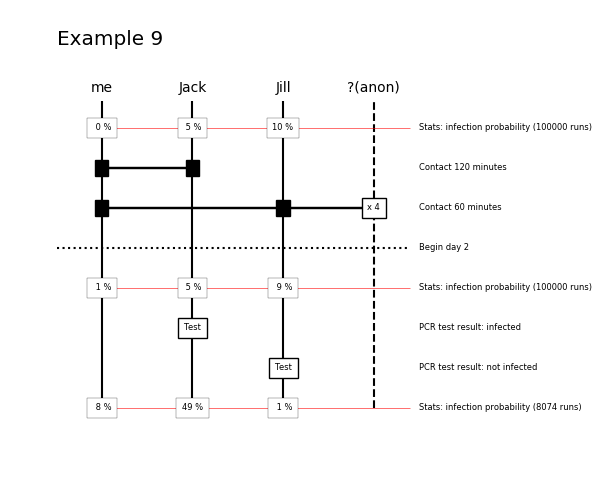
\includegraphics{SimRiskExample.png}
\caption{SimRiskExample.png}
\end{figure}

    This example shows a contact schedule for three named individuals (me,
Jack and Jill) over a period of two days. There are eleven events.

The following code specifies the model to be simulated:

\begin{verbatim}
function example9()::Model
    m = Model("Example 9")
    # day 1
    notePerson!(m, "me", infectedProbability=0.00, maskedProbability=0.500)
    notePerson!(m, "Jack", infectedProbability=0.05, maskedProbability=0.000)
    notePerson!(m, "Jill", infectedProbability=0.10, maskedProbability=1.00)
    noteStats!(m)
    noteContact!(m, ["me", "Jack"], minutes=120)
    noteContact!(m, ["me", "Jill"], anonymousNumber=4, minutes=60)
    # day 2
    noteNewDay!(m)
    noteStats!(m)
    noteTest!(m, "Jack", PCRTest, true)
    noteTest!(m, "Jill", PCRTest, false)
    noteStats!(m)
    return m
end    
\end{verbatim}

\begin{itemize}
\item
  The first three \texttt{notePerson!} events specify the three named
  individuals in the model.

  \begin{itemize}
  \tightlist
  \item
    The first named person, \texttt{me}, starts every simulation run
    uninfected. I wear a mask half of the time. (This means that I start
    off masked in half of the simulation runs.)
  \item
    The second named person, \texttt{Jack}, starts off each simulation
    run with a 5\% chance of being infected. Jack never wears a mask.
  \item
    The third named person, \texttt{Jill}, starts off each simulation
    run with a 10\% chance of being infected. Jill always wears an N95
    mask with 95\% filtration ability when Jill is the ``sender'' or
    when Jill is the ``receiver''.
  \end{itemize}
\item
  The first \texttt{Stats} event gathers statistics, showing the initial
  0\% / 5\% / 10\% infection rates for me, Jack, and Jill. These are
  computed using 100000 simulation runs, and show the number of such
  runs wherein each party is infected.
\item
  The next two events on day 1 are contact events:

  \begin{itemize}
  \tightlist
  \item
    Jack and I have a two-hour meeting.
  \item
    Jill and I, together with four anonymous other individuals, have a
    one-hour lunch.
  \end{itemize}
\item
  The next event is the beginning of day two. In some simulation runs,
  some individuals recover in this transition (about 1/14 of them will
  do so).
\item
  The next event is a \texttt{Stats} event, showing that me, Jack, and
  Jill have infection probabilities of 1\% / 5\% / 9\%. (Remember that
  Jill always wears a mask!) These percentages are percentages of the
  100000 simulation runs wherein each party is infected.
\item
  The next two events are \texttt{Test} events:

  \begin{itemize}
  \tightlist
  \item
    a PCR \texttt{Test} event for Jack; it shows him to be infected.
    This PCR test has a 5\% false-positive and a 5\% false-negative
    rate.
  \item
    a similar PCR \texttt{Test} event for Jill, it shows her to be
    uninfected.
  \end{itemize}
\item
  The final event is a \texttt{Stats} showing me, Jack, and Jill to be
  infected with respective probabilities 8\%, 49\%, and 1\%. Note that
  only 8074 simulation runs showed Jack testing positive and Jill
  testing negative; the other simulation runs are discarded at this
  point. The percentages given are the percentages of the 8074
  simulation runs that gave results for the two Test events that were
  consistent with the observed Test results, that showed each of the
  three named individuals being infected.
\end{itemize}

In general, events may have stochastic effects, which is why simulation
is needed to determine the probability that a named individual is
infected at the end of the schedule. A random number seed and
appropriate cryptographic for the simulation allow the use of
pseudorandomness here, for reproducibility.

Note that the infection probabilities of anonymous individuals are not
estimated; each contact including anonymous individuals is assumed to
include freshly-minted anonymous individuals with infection probability
equal to the overall prevalence rate of infection.

This is clearly a simplistic model that could be made more realistic in
a number of ways.
\newpage
    \hypertarget{disease-states}{%
\section{Disease States}\label{disease-states}}

    \begin{tcolorbox}[breakable, size=fbox, boxrule=1pt, pad at break*=1mm,colback=cellbackground, colframe=cellborder]
\prompt{In}{incolor}{1}{\boxspacing}
\begin{Verbatim}[commandchars=\\\{\}]
\PY{c}{\PYZsh{} We represent the following disease states:}
\PY{c}{\PYZsh{}     Susceptible  I1 I2 ... ILast  Recovered}
\PY{c}{\PYZsh{} We use ILast = I14 here.  Later versions may make \PYZdq{}14\PYZdq{} variable.}
\PY{c}{\PYZsh{} These are \PYZdq{}daily\PYZdq{} states, giving the disease state at the end of the day.}
\PY{c}{\PYZsh{} States I1 ... I14 are \PYZdq{}infected\PYZdq{} states; these states are not necessarily \PYZdq{}infectious\PYZdq{}.}
\PY{c}{\PYZsh{} An infected person progresses from state I1 to state Recovered, one state at a time per day.}
\PY{c}{\PYZsh{} Moving from state Susceptible to state I1 is the initial infection.}
\PY{c}{\PYZsh{} Moving from state I14 to state Recovered is \PYZdq{}recovery\PYZdq{}.}
\PY{c}{\PYZsh{} We represent these states as integers as follows:}
\PY{c}{\PYZsh{} a state Id (where d is an integer) is the disease state at the end of the d\PYZhy{}th day of infection.}
\PY{c}{\PYZsh{} So, I1 is the end of the first day of infection, etc.}
\PY{c}{\PYZsh{} We use the encoding of disease states as integers:}
\PY{c}{\PYZsh{}    Susceptible = 0}
\PY{c}{\PYZsh{}    I1 ... I14 = 1 ... 14}
\PY{c}{\PYZsh{}    Recovered = 15}

\PY{k}{struct} \PY{n}{DiseaseState} \PY{o}{\PYZlt{}:} \PY{k+kt}{Integer}
    \PY{n}{ds}\PY{o}{::}\PY{k+kt}{Int64}
\PY{k}{end}
\PY{k+kt}{Int64}\PY{p}{(}\PY{n}{x}\PY{o}{::}\PY{n}{DiseaseState}\PY{p}{)} \PY{o}{=} \PY{n}{x}\PY{o}{.}\PY{n}{ds} 
\PY{k}{import} \PY{n}{Base}\PY{o}{.\PYZlt{}}
\PY{o}{\PYZlt{}}\PY{p}{(}\PY{n}{x}\PY{o}{::}\PY{n}{DiseaseState}\PY{p}{,} \PY{n}{y}\PY{o}{::}\PY{n}{DiseaseState}\PY{p}{)} \PY{o}{=} \PY{p}{(}\PY{n}{x}\PY{o}{.}\PY{n}{ds} \PY{o}{\PYZlt{}} \PY{n}{y}\PY{o}{.}\PY{n}{ds}\PY{p}{)}

\PY{c}{\PYZsh{} Although Julia uses 1\PYZhy{}indexing, we start DiseaseState at 0 (= Susceptible);}
\PY{c}{\PYZsh{} so arrays that are indexed by DiseaseState are 0\PYZhy{}indexed}
\PY{k+kd}{const} \PY{n}{Susceptible} \PY{o}{=} \PY{n}{DiseaseState}\PY{p}{(}\PY{l+m+mi}{0}\PY{p}{)}
\PY{k+kd}{const} \PY{n}{I1} \PY{o}{=} \PY{n}{DiseaseState}\PY{p}{(}\PY{l+m+mi}{1}\PY{p}{)}           \PY{c}{\PYZsh{} when person is infected, they move to state I1}
\PY{k+kd}{const} \PY{n}{ILast} \PY{o}{=} \PY{n}{DiseaseState}\PY{p}{(}\PY{l+m+mi}{14}\PY{p}{)}       \PY{c}{\PYZsh{} last infected disease state}
\PY{k+kd}{const} \PY{n}{Recovered} \PY{o}{=} \PY{n}{DiseaseState}\PY{p}{(}\PY{l+m+mi}{15}\PY{p}{)}

\PY{n}{DiseaseState}\PY{p}{(}\PY{p}{)} \PY{o}{=} \PY{n}{Susceptible}         \PY{c}{\PYZsh{} default starting disease state}

\PY{n}{infected}\PY{p}{(}\PY{n}{x}\PY{o}{::}\PY{n}{DiseaseState}\PY{p}{)} \PY{o}{=} \PY{p}{(}\PY{n}{Susceptible} \PY{o}{\PYZlt{}} \PY{n}{x} \PY{o}{\PYZlt{}} \PY{n}{Recovered}\PY{p}{)}

\PY{n}{SymptomOnset} \PY{o}{=} \PY{n}{DiseaseState}\PY{p}{(}\PY{l+m+mi}{5}\PY{p}{)}  \PY{c}{\PYZsh{} if symptomatic, symptoms start on day 5}

\PY{c}{\PYZsh{} if state ds on day d, give state on next day}
\PY{k}{function} \PY{n}{nextDiseaseState}\PY{p}{(}\PY{n}{ds}\PY{o}{::}\PY{n}{DiseaseState}\PY{p}{)}
    \PY{p}{(}\PY{n}{ds} \PY{o}{==} \PY{n}{Susceptible}\PY{p}{)} \PY{o}{\PYZam{}\PYZam{}} \PY{k}{return} \PY{n}{ds}
    \PY{p}{(}\PY{n}{ds} \PY{o}{==} \PY{n}{Recovered}\PY{p}{)} \PY{o}{\PYZam{}\PYZam{}} \PY{k}{return} \PY{n}{ds}
    \PY{k}{return} \PY{n}{DiseaseState}\PY{p}{(}\PY{k+kt}{Int}\PY{p}{(}\PY{n}{ds}\PY{o}{.}\PY{n}{ds}\PY{p}{)}\PY{o}{+}\PY{l+m+mi}{1}\PY{p}{)}
\PY{k}{end}
\end{Verbatim}
\end{tcolorbox}

            \begin{tcolorbox}[breakable, size=fbox, boxrule=.5pt, pad at break*=1mm, opacityfill=0]
\prompt{Out}{outcolor}{1}{\boxspacing}
\begin{Verbatim}[commandchars=\\\{\}]
nextDiseaseState (generic function with 1 method)
\end{Verbatim}
\end{tcolorbox}
        
    \begin{tcolorbox}[breakable, size=fbox, boxrule=1pt, pad at break*=1mm,colback=cellbackground, colframe=cellborder]
\prompt{In}{incolor}{2}{\boxspacing}
\begin{Verbatim}[commandchars=\\\{\}]
\PY{c}{\PYZsh{} infectiousness as a function of DiseaseState}
\PY{c}{\PYZsh{} average of infected states is 1.000}
\PY{c}{\PYZsh{} using Pkg ;}
\PY{c}{\PYZsh{} Pkg.add(\PYZdq{}OffsetArrays\PYZdq{}) ;}
\PY{k}{using} \PY{n}{OffsetArrays} \PY{p}{;}

\PY{n}{defaultInfectiousness} \PY{o}{=}      \PY{c}{\PYZsh{} improve this list?}
    \PY{n}{OffsetArray}\PY{p}{(}\PY{p}{[}\PY{l+m+mi}{0}\PY{p}{,} 
                 \PY{l+m+mi}{0}\PY{p}{,} \PY{l+m+mi}{1}\PY{p}{,} \PY{l+m+mi}{2}\PY{p}{,} \PY{l+m+mi}{2}\PY{p}{,} \PY{l+m+mi}{2}\PY{p}{,} \PY{l+m+mi}{2}\PY{p}{,} \PY{l+m+mi}{2}\PY{p}{,} \PY{l+m+mi}{1}\PY{p}{,} \PY{l+m+mi}{1}\PY{p}{,} \PY{l+m+mi}{1}\PY{p}{,} \PY{l+m+mi}{1}\PY{p}{,} \PY{l+m+mi}{1}\PY{p}{,} \PY{l+m+mi}{1}\PY{p}{,} \PY{l+m+mi}{1}\PY{p}{,}  \PY{c}{\PYZsh{} note 0 for I1}
                 \PY{l+m+mi}{0}\PY{p}{]}\PY{p}{,}
                \PY{l+m+mi}{0}\PY{o}{:}\PY{l+m+mi}{15}\PY{p}{)} \PY{o}{*} \PY{p}{(}\PY{l+m+mf}{14.0} \PY{o}{/} \PY{l+m+mf}{18.0}\PY{p}{)}\PY{p}{;}
\end{Verbatim}
\end{tcolorbox}

    \hypertarget{tests}{%
\subsection{Tests}\label{tests}}

When using a fixed contact schedule, we assume that testing affects the
\emph{transmission probability} but not the \emph{contact schedule} or
other observable attributes such as whether a person is wearing a mask.

    \begin{tcolorbox}[breakable, size=fbox, boxrule=1pt, pad at break*=1mm,colback=cellbackground, colframe=cellborder]
\prompt{In}{incolor}{3}{\boxspacing}
\begin{Verbatim}[commandchars=\\\{\}]
\PY{k}{struct} \PY{n}{TestType}
    \PY{n}{name}\PY{o}{::}\PY{n}{String}         \PY{c}{\PYZsh{} name of test type}
    \PY{n}{P\PYZus{}det}\PY{o}{::}\PY{k+kt}{Real}          \PY{c}{\PYZsh{} Probability of detecting infection }
                         \PY{c}{\PYZsh{}     = P(pos test result | infected)}
                         \PY{c}{\PYZsh{}     = sensitivity}
    \PY{n}{P\PYZus{}FA}\PY{o}{::}\PY{k+kt}{Real}           \PY{c}{\PYZsh{} Probability of a false alarm }
                         \PY{c}{\PYZsh{}     = P(pos test result | uninfected)}
                         \PY{c}{\PYZsh{}     = 1 \PYZhy{} specificity}
\PY{k}{end}

\PY{n}{PerfectTest} \PY{o}{=} \PY{n}{TestType}\PY{p}{(}\PY{l+s}{\PYZdq{}}\PY{l+s}{P}\PY{l+s}{e}\PY{l+s}{r}\PY{l+s}{f}\PY{l+s}{e}\PY{l+s}{c}\PY{l+s}{t}\PY{l+s}{\PYZdq{}}\PY{p}{,} \PY{l+m+mf}{1.0}\PY{p}{,} \PY{l+m+mf}{0.0}\PY{p}{)}       \PY{c}{\PYZsh{} this test is always right}
\PY{n}{PCRTest} \PY{o}{=} \PY{n}{TestType}\PY{p}{(}\PY{l+s}{\PYZdq{}}\PY{l+s}{P}\PY{l+s}{C}\PY{l+s}{R}\PY{l+s}{\PYZdq{}}\PY{p}{,} \PY{l+m+mf}{0.95}\PY{p}{,} \PY{l+m+mf}{0.05}\PY{p}{)}             \PY{c}{\PYZsh{} check (if adjust here, also adjust examples)}
\PY{n}{OtherTest} \PY{o}{=} \PY{n}{TestType}\PY{p}{(}\PY{l+s}{\PYZdq{}}\PY{l+s}{O}\PY{l+s}{t}\PY{l+s}{h}\PY{l+s}{e}\PY{l+s}{r}\PY{l+s}{\PYZdq{}}\PY{p}{,} \PY{l+m+mf}{0.90}\PY{p}{,} \PY{l+m+mf}{0.10}\PY{p}{)}         \PY{c}{\PYZsh{} for comparison purposes, not a real test}
\end{Verbatim}
\end{tcolorbox}

            \begin{tcolorbox}[breakable, size=fbox, boxrule=.5pt, pad at break*=1mm, opacityfill=0]
\prompt{Out}{outcolor}{3}{\boxspacing}
\begin{Verbatim}[commandchars=\\\{\}]
TestType("Other", 0.9, 0.1)
\end{Verbatim}
\end{tcolorbox}
        
    \hypertarget{masks}{%
\subsection{Masks}\label{masks}}

Same for masks; being masked affects transmission probability but not
the event schedule.

A MaskType is defined by is filtration efficiencies (separately as
source and as recipient).

    \begin{tcolorbox}[breakable, size=fbox, boxrule=1pt, pad at break*=1mm,colback=cellbackground, colframe=cellborder]
\prompt{In}{incolor}{4}{\boxspacing}
\begin{Verbatim}[commandchars=\\\{\}]
\PY{k}{struct} \PY{n}{MaskType}
    \PY{n}{sourceMaskTransmission}\PY{o}{::}\PY{k+kt}{Real}    \PY{c}{\PYZsh{} 1 \PYZhy{} filtrationEfficiency for source, if source wearing this mask type}
    \PY{n}{recipientMaskTransmission}\PY{o}{::}\PY{k+kt}{Real} \PY{c}{\PYZsh{} 1 \PYZhy{} filtrationEfficiency for recipient, if recipient wearing this mask type}
\PY{k}{end}

\PY{n}{N95} \PY{o}{=} \PY{n}{MaskType}\PY{p}{(}\PY{l+m+mf}{0.05}\PY{p}{,} \PY{l+m+mf}{0.05}\PY{p}{)}          \PY{c}{\PYZsh{} Check numbers}
\PY{n}{Surgical} \PY{o}{=} \PY{n}{MaskType}\PY{p}{(}\PY{l+m+mf}{0.30}\PY{p}{,} \PY{l+m+mf}{0.20}\PY{p}{)}     \PY{c}{\PYZsh{} Check numbers}
\PY{n}{NoMask} \PY{o}{=} \PY{n}{MaskType}\PY{p}{(}\PY{l+m+mf}{1.00}\PY{p}{,} \PY{l+m+mf}{1.00}\PY{p}{)}
\end{Verbatim}
\end{tcolorbox}

            \begin{tcolorbox}[breakable, size=fbox, boxrule=.5pt, pad at break*=1mm, opacityfill=0]
\prompt{Out}{outcolor}{4}{\boxspacing}
\begin{Verbatim}[commandchars=\\\{\}]
MaskType(1.0, 1.0)
\end{Verbatim}
\end{tcolorbox}
        
    \hypertarget{quarantine}{%
\subsection{Quarantine}\label{quarantine}}

We do not explicitly model quarantining; we assume that the given events
already incorporate any effects that quarantining might have had.
\newpage
    \hypertarget{people}{%
\section{People}\label{people}}

Each person is represented in the simulation by a Person object. We
might also call this a \emph{node} or a \emph{vertex}, using
graph-theoretic terminology.

The node contains a number of attributes, which may change value as the
simulation progresses; the Person object is a \emph{mutable} data
structure.

    \begin{tcolorbox}[breakable, size=fbox, boxrule=1pt, pad at break*=1mm,colback=cellbackground, colframe=cellborder]
\prompt{In}{incolor}{5}{\boxspacing}
\begin{Verbatim}[commandchars=\\\{\}]
\PY{k}{struct} \PY{n}{VisibleState}
    \PY{c}{\PYZsh{} represents state elements that are visible and may affect disease transmission}
    \PY{n}{mask}\PY{o}{::}\PY{n}{MaskType}
\PY{k}{end}
\PY{c}{\PYZsh{} Default VisibleState is unmasked}
\PY{n}{VisibleState}\PY{p}{(}\PY{p}{)} \PY{o}{=} \PY{n}{VisibleState}\PY{p}{(}\PY{n}{NoMask}\PY{p}{)}
\end{Verbatim}
\end{tcolorbox}

            \begin{tcolorbox}[breakable, size=fbox, boxrule=.5pt, pad at break*=1mm, opacityfill=0]
\prompt{Out}{outcolor}{5}{\boxspacing}
\begin{Verbatim}[commandchars=\\\{\}]
VisibleState
\end{Verbatim}
\end{tcolorbox}
        
    \begin{tcolorbox}[breakable, size=fbox, boxrule=1pt, pad at break*=1mm,colback=cellbackground, colframe=cellborder]
\prompt{In}{incolor}{6}{\boxspacing}
\begin{Verbatim}[commandchars=\\\{\}]
\PY{k}{mutable} \PY{k}{struct} \PY{n}{Person} \PY{c}{\PYZsh{} aka Agent}

    \PY{c}{\PYZsh{} static attributes of person}
    \PY{n}{personID}\PY{o}{::}\PY{n}{String}

    \PY{c}{\PYZsh{} per\PYZhy{}run attributes of person}
    \PY{n}{asymptomatic}\PY{o}{::}\PY{k+kt}{Bool}                   \PY{c}{\PYZsh{} whether asymptomatic on this run}
    
    \PY{c}{\PYZsh{} per\PYZhy{}run dynamic attributes of person (changes over time)}
    \PY{n}{diseaseState}\PY{o}{::}\PY{n}{DiseaseState}
    \PY{n}{visibleState}\PY{o}{::}\PY{n}{VisibleState}
\PY{k}{end}
\end{Verbatim}
\end{tcolorbox}
\newpage
    \hypertarget{key-additional-concepts}{%
\section{Key Additional Concepts}\label{key-additional-concepts}}

    \hypertarget{global-parameters}{%
\subsection{Global parameters}\label{global-parameters}}

One struct gives a list of global parameters, such as prevalence rate,
in a timeless manner.

    \begin{tcolorbox}[breakable, size=fbox, boxrule=1pt, pad at break*=1mm,colback=cellbackground, colframe=cellborder]
\prompt{In}{incolor}{7}{\boxspacing}
\begin{Verbatim}[commandchars=\\\{\}]
\PY{k}{mutable} \PY{k}{struct} \PY{n}{GlobalParameters}
    \PY{c}{\PYZsh{} parameters for random named people}
    \PY{n}{infectedProbability}\PY{o}{::}\PY{k+kt}{Real}                  \PY{c}{\PYZsh{} probability that a random person is infected}
    \PY{n}{maskedProbability}\PY{o}{::}\PY{k+kt}{Real}                    \PY{c}{\PYZsh{} probability that a random person is masked}
    \PY{n}{asymptomaticProbability}\PY{o}{::}\PY{k+kt}{Real}              \PY{c}{\PYZsh{} probability that a random person is asymptomatic}
    \PY{c}{\PYZsh{} same parameters for random anonymous people}
    \PY{n}{anonymousInfectedProbability}\PY{o}{::}\PY{k+kt}{Real}
    \PY{n}{anonymousMaskedProbability}\PY{o}{::}\PY{k+kt}{Real}
    \PY{n}{anonymousAsymptomaticProbability}\PY{o}{::}\PY{k+kt}{Real}

    \PY{c}{\PYZsh{} ContactEvent parameters}

    \PY{c}{\PYZsh{} A contact with a give dose (arbitrary units) between two maskless individuals has a probability}
    \PY{c}{\PYZsh{} of transmission of 1 \PYZhy{} exp(\PYZhy{}dose*transmissionConstant)}
    \PY{n}{transmissionConstant}\PY{o}{::}\PY{k+kt}{Real} 
    \PY{n}{asymptomaticFactor}\PY{o}{::}\PY{k+kt}{Real}   \PY{c}{\PYZsh{} reduce dose by this factor if source is asymptomatic}
    
    \PY{c}{\PYZsh{} infectiousness as a function of DiseaseState (indices will be \PYZhy{}1:infectionDurationDays)}
    \PY{n}{infectiousness}\PY{o}{::}\PY{n}{OffsetArray}\PY{p}{\PYZob{}}\PY{k+kt}{Float64}\PY{p}{,}\PY{l+m+mi}{1}\PY{p}{,}\PY{k+kt}{Array}\PY{p}{\PYZob{}}\PY{k+kt}{Float64}\PY{p}{,}\PY{l+m+mi}{1}\PY{p}{\PYZcb{}}\PY{p}{\PYZcb{}}
\PY{k}{end}

\PY{c}{\PYZsh{} default parameters for named people}
\PY{n}{defaultInfectedProbability} \PY{o}{=} \PY{l+m+mf}{0.02}      \PY{c}{\PYZsh{} prevalence in community}
\PY{n}{defaultMaskedProbability} \PY{o}{=} \PY{l+m+mf}{0.000}
\PY{n}{defaultAsymptomaticProbability} \PY{o}{=} \PY{l+m+mf}{0.40}  \PY{c}{\PYZsh{} https://www.cdc.gov/coronavirus/2019\PYZhy{}ncov/hcp/planning\PYZhy{}scenarios.html}
\PY{c}{\PYZsh{} same parameters for anonymous people}
\PY{n}{defaultAnonymousInfectedProbability} \PY{o}{=} \PY{n}{defaultInfectedProbability}
\PY{n}{defaultAnonymousMaskedProbability} \PY{o}{=} \PY{n}{defaultMaskedProbability}
\PY{n}{defaultAnonymousAsymptomaticProbability} \PY{o}{=} \PY{n}{defaultAsymptomaticProbability}

\PY{c}{\PYZsh{} We choose the transmission constant so that }
\PY{c}{\PYZsh{} a fifteen\PYZhy{}minute contact has a 5\PYZpc{} chance of transmission.}
\PY{n}{defaultContactDuration} \PY{o}{=} \PY{l+m+mf}{15.0}                     \PY{c}{\PYZsh{} 15 minutes in close contact}
\PY{n}{defaultContactTransmissionProbability} \PY{o}{=} \PY{l+m+mf}{0.05}      \PY{c}{\PYZsh{} yields 5\PYZpc{} chance of transmission of disease}
\PY{n}{defaultTransmissionConstant} \PY{o}{=} \PY{n}{log}\PY{p}{(}\PY{l+m+mi}{1}\PY{o}{\PYZhy{}}\PY{n}{defaultContactTransmissionProbability}\PY{p}{)}\PY{o}{/} \PY{p}{(}\PY{o}{\PYZhy{}}\PY{n}{defaultContactDuration}\PY{p}{)}
\PY{n}{defaultAsymptomaticFactor} \PY{o}{=} \PY{l+m+mf}{0.75} \PY{c}{\PYZsh{} from https://www.cdc.gov/coronavirus/2019\PYZhy{}ncov/hcp/planning\PYZhy{}scenarios.html}

\PY{n}{defaultGlobalParameters} \PY{o}{=} 
    \PY{n}{GlobalParameters}\PY{p}{(} \PY{n}{defaultInfectedProbability}\PY{p}{,}
                      \PY{n}{defaultMaskedProbability}\PY{p}{,}
                      \PY{n}{defaultAsymptomaticProbability}\PY{p}{,}
                      \PY{n}{defaultAnonymousInfectedProbability}\PY{p}{,}
                      \PY{n}{defaultAnonymousMaskedProbability}\PY{p}{,}
                      \PY{n}{defaultAnonymousAsymptomaticProbability}\PY{p}{,}
                      \PY{n}{defaultTransmissionConstant}\PY{p}{,}
                      \PY{n}{defaultAsymptomaticFactor}\PY{p}{,}
                      \PY{n}{defaultInfectiousness}
                    \PY{p}{)}
\end{Verbatim}
\end{tcolorbox}

            \begin{tcolorbox}[breakable, size=fbox, boxrule=.5pt, pad at break*=1mm, opacityfill=0]
\prompt{Out}{outcolor}{7}{\boxspacing}
\begin{Verbatim}[commandchars=\\\{\}]
GlobalParameters(0.02, 0.0, 0.4, 0.02, 0.0, 0.4, 0.0034195529591700387, 0.75,
[0.0, 0.0, 0.777778, 1.55556, 1.55556, 1.55556, 1.55556, 1.55556, 0.777778,
0.777778, 0.777778, 0.777778, 0.777778, 0.777778, 0.777778, 0.0])
\end{Verbatim}
\end{tcolorbox}
        \newpage
    \hypertarget{events}{%
\section{Events}\label{events}}

    Each event specifies how the model state is to be updated. The update
may be probabilistic.

For example, an event might say that if Bob is infected but Alice is
not, then Alice becomes infected with probability 15\%.

The effects of an event may depend on the attributes of the input nodes.
For example, in our example transmission probability may be smaller if
either Alice and Bob are wearing masks, and smaller still if both are
wearing masks.

Each event in effect runs some program, that takes as input a person or
a set of people, and updates the state of that person or those people.

    \begin{tcolorbox}[breakable, size=fbox, boxrule=1pt, pad at break*=1mm,colback=cellbackground, colframe=cellborder]
\prompt{In}{incolor}{8}{\boxspacing}
\begin{Verbatim}[commandchars=\\\{\}]
\PY{k}{struct} \PY{n}{DefaultParametersEvent}      \PY{c}{\PYZsh{} set model default global parameters to these values}
    \PY{n}{infected}\PY{o}{::}\PY{k+kt}{Real}
    \PY{n}{masked}\PY{o}{::}\PY{k+kt}{Real}
\PY{k}{end}
\end{Verbatim}
\end{tcolorbox}

    \begin{tcolorbox}[breakable, size=fbox, boxrule=1pt, pad at break*=1mm,colback=cellbackground, colframe=cellborder]
\prompt{In}{incolor}{9}{\boxspacing}
\begin{Verbatim}[commandchars=\\\{\}]
\PY{k}{struct} \PY{n}{NewPersonEvent}
    \PY{n}{person}\PY{o}{::}\PY{n}{Person}                 \PY{c}{\PYZsh{} person created first, then NewPersonEvent}
    \PY{n}{infectedProbability}\PY{o}{::}\PY{k+kt}{Real}      \PY{c}{\PYZsh{} e.g. prevalance of infection in the population individual is drawn from}
                                   \PY{c}{\PYZsh{} assume equally likely to be any of I1...ILast}
                                   \PY{c}{\PYZsh{} Todo: update for other distributions.}
    \PY{n}{maskedProbability}\PY{o}{::}\PY{k+kt}{Real}        \PY{c}{\PYZsh{} probability that new individual is masked}
    \PY{n}{asymptomaticProbability}\PY{o}{::}\PY{k+kt}{Real}  \PY{c}{\PYZsh{} probability that new individual is asymptomatic}
    
\PY{k}{end}
\end{Verbatim}
\end{tcolorbox}

    \begin{tcolorbox}[breakable, size=fbox, boxrule=1pt, pad at break*=1mm,colback=cellbackground, colframe=cellborder]
\prompt{In}{incolor}{10}{\boxspacing}
\begin{Verbatim}[commandchars=\\\{\}]
\PY{k}{struct} \PY{n}{NewDayEvent}
\PY{k}{end}
\end{Verbatim}
\end{tcolorbox}

    \begin{tcolorbox}[breakable, size=fbox, boxrule=1pt, pad at break*=1mm,colback=cellbackground, colframe=cellborder]
\prompt{In}{incolor}{11}{\boxspacing}
\begin{Verbatim}[commandchars=\\\{\}]
\PY{c}{\PYZsh{} A Test Event is a measurement of the disease state of a person,}
\PY{c}{\PYZsh{} together with a required (reported) value for that test result.}
\PY{k}{struct} \PY{n}{TestEvent}
    \PY{n}{person}\PY{o}{::}\PY{n}{Person}
    \PY{n}{testType}\PY{o}{::}\PY{n}{TestType}
    \PY{n}{reportedTestResult}\PY{o}{::}\PY{k+kt}{Bool}       \PY{c}{\PYZsh{} simulated test result must match this reportedTestRestult}
                                   \PY{c}{\PYZsh{} or else simulation run doesn\PYZsq{}t count}
\PY{k}{end}
\end{Verbatim}
\end{tcolorbox}

    \begin{tcolorbox}[breakable, size=fbox, boxrule=1pt, pad at break*=1mm,colback=cellbackground, colframe=cellborder]
\prompt{In}{incolor}{12}{\boxspacing}
\begin{Verbatim}[commandchars=\\\{\}]
\PY{k}{struct} \PY{n}{SymptomOnsetEvent}
    \PY{n}{person}\PY{o}{::}\PY{n}{Person}
    \PY{n}{reportedSymptomOnsetResult}\PY{o}{::}\PY{k+kt}{Bool}  \PY{c}{\PYZsh{} true if symptoms start on this day}
\PY{k}{end}
\end{Verbatim}
\end{tcolorbox}

    \begin{tcolorbox}[breakable, size=fbox, boxrule=1pt, pad at break*=1mm,colback=cellbackground, colframe=cellborder]
\prompt{In}{incolor}{13}{\boxspacing}
\begin{Verbatim}[commandchars=\\\{\}]
\PY{k}{struct} \PY{n}{ContactEvent}  \PY{c}{\PYZsh{} Close Contact Event between two or more people }
                     \PY{c}{\PYZsh{} An Int means that many people with default parameter settings}
                     \PY{c}{\PYZsh{} (Vertical line segment joining two or more horizontal Person lines)}
    \PY{n}{minutes}\PY{o}{::}\PY{k+kt}{Int} 
    \PY{n}{people}\PY{o}{::}\PY{k+kt}{Array}\PY{p}{\PYZob{}}\PY{n}{Person}\PY{p}{\PYZcb{}}
    \PY{n}{anonymousNumber}\PY{o}{::}\PY{k+kt}{Int}
    \PY{n}{anonymousInfectedProbability}\PY{o}{::}\PY{k+kt}{Real}
    \PY{n}{anonymousMaskedProbability}\PY{o}{::}\PY{k+kt}{Real}
    \PY{n}{anonymousAsymptomaticProbability}\PY{o}{::}\PY{k+kt}{Real}
\PY{k}{end}
\end{Verbatim}
\end{tcolorbox}

    \begin{tcolorbox}[breakable, size=fbox, boxrule=1pt, pad at break*=1mm,colback=cellbackground, colframe=cellborder]
\prompt{In}{incolor}{14}{\boxspacing}
\begin{Verbatim}[commandchars=\\\{\}]
\PY{k}{struct} \PY{n}{MaskEvent}           \PY{c}{\PYZsh{} cause individual to become masked (with given MaskType)}
    \PY{n}{person}\PY{o}{::}\PY{n}{Person}
    \PY{n}{mask}\PY{o}{::}\PY{n}{MaskType} 
\PY{k}{end}
\end{Verbatim}
\end{tcolorbox}

    \begin{tcolorbox}[breakable, size=fbox, boxrule=1pt, pad at break*=1mm,colback=cellbackground, colframe=cellborder]
\prompt{In}{incolor}{15}{\boxspacing}
\begin{Verbatim}[commandchars=\\\{\}]
\PY{k}{struct} \PY{n}{StatsEvent}           \PY{c}{\PYZsh{} collect statistics: is each named person infected?}
\PY{k}{end}
\end{Verbatim}
\end{tcolorbox}

    \begin{tcolorbox}[breakable, size=fbox, boxrule=1pt, pad at break*=1mm,colback=cellbackground, colframe=cellborder]
\prompt{In}{incolor}{16}{\boxspacing}
\begin{Verbatim}[commandchars=\\\{\}]
\PY{n}{Event} \PY{o}{=} \PY{k+kt}{Union}\PY{p}{\PYZob{}}\PY{n}{DefaultParametersEvent}\PY{p}{,} \PY{n}{NewPersonEvent}\PY{p}{,} \PY{n}{NewDayEvent}\PY{p}{,} 
              \PY{n}{TestEvent}\PY{p}{,} \PY{n}{SymptomOnsetEvent}\PY{p}{,} \PY{n}{ContactEvent}\PY{p}{,} \PY{n}{MaskEvent}\PY{p}{,} \PY{n}{StatsEvent}\PY{p}{\PYZcb{}}
\end{Verbatim}
\end{tcolorbox}

            \begin{tcolorbox}[breakable, size=fbox, boxrule=.5pt, pad at break*=1mm, opacityfill=0]
\prompt{Out}{outcolor}{16}{\boxspacing}
\begin{Verbatim}[commandchars=\\\{\}]
Union\{NewDayEvent, StatsEvent, ContactEvent, DefaultParametersEvent, MaskEvent,
NewPersonEvent, SymptomOnsetEvent, TestEvent\}
\end{Verbatim}
\end{tcolorbox}
        \newpage
    \hypertarget{models}{%
\section{Models}\label{models}}

The model contains * global parameters, * a list of all named people in
the model, * an (ordered) \emph{event list} of \emph{events} (The event
list is a \emph{schedule} of events to be run by the scheduler; the
events happen in the specified order), and * the number of StatsEvent
entries in the event list

    \begin{tcolorbox}[breakable, size=fbox, boxrule=1pt, pad at break*=1mm,colback=cellbackground, colframe=cellborder]
\prompt{In}{incolor}{17}{\boxspacing}
\begin{Verbatim}[commandchars=\\\{\}]
\PY{k}{mutable} \PY{k}{struct} \PY{n}{Model}
    \PY{n}{params}\PY{o}{::}\PY{n}{GlobalParameters}
    \PY{n}{people}\PY{o}{::}\PY{k+kt}{Array}\PY{p}{\PYZob{}}\PY{n}{Person}\PY{p}{\PYZcb{}}     \PY{c}{\PYZsh{} all people in model}
    \PY{n}{events}\PY{o}{::}\PY{k+kt}{Array}\PY{p}{\PYZob{}}\PY{n}{Event}\PY{p}{\PYZcb{}}      \PY{c}{\PYZsh{} all events in model, ordered by time of occurrence}
    \PY{n}{name}\PY{o}{::}\PY{n}{String}              \PY{c}{\PYZsh{} name of the model}
    \PY{n}{nStats}\PY{o}{::}\PY{k+kt}{Int}               \PY{c}{\PYZsh{} number of stats events in event list}
    \PY{n}{stats}\PY{o}{::}\PY{k+kt}{Dict}               \PY{c}{\PYZsh{} statistics gathered}
\PY{k}{end}
\PY{n}{Model}\PY{p}{(}\PY{p}{)} \PY{o}{=} \PY{n}{Model}\PY{p}{(}\PY{n}{defaultGlobalParameters}\PY{p}{,} \PY{p}{[}\PY{p}{]}\PY{p}{,} \PY{p}{[}\PY{p}{]}\PY{p}{,} \PY{l+s}{\PYZdq{}}\PY{l+s}{\PYZdq{}}\PY{p}{,} \PY{l+m+mi}{1}\PY{p}{,} \PY{k+kt}{Dict}\PY{p}{(}\PY{p}{)}\PY{p}{)}
\PY{n}{Model}\PY{p}{(}\PY{n}{name}\PY{o}{::}\PY{n}{String}\PY{p}{)} \PY{o}{=} \PY{n}{Model}\PY{p}{(}\PY{n}{defaultGlobalParameters}\PY{p}{,} \PY{p}{[}\PY{p}{]}\PY{p}{,} \PY{p}{[}\PY{p}{]}\PY{p}{,} \PY{n}{name}\PY{p}{,} \PY{l+m+mi}{1}\PY{p}{,} \PY{k+kt}{Dict}\PY{p}{(}\PY{p}{)}\PY{p}{)}
\end{Verbatim}
\end{tcolorbox}

            \begin{tcolorbox}[breakable, size=fbox, boxrule=.5pt, pad at break*=1mm, opacityfill=0]
\prompt{Out}{outcolor}{17}{\boxspacing}
\begin{Verbatim}[commandchars=\\\{\}]
Model
\end{Verbatim}
\end{tcolorbox}
        
    \hypertarget{model-initialization-and-specification}{%
\subsection{Model initialization and
specification}\label{model-initialization-and-specification}}

This section gives the tools for specifying a model.

The model must be complete specified before simulation can begin.

The model-specification API consists of number of functions, each of
whose name begins with \texttt{note}, and take as their first argument
the model being specified.

Some of the main model-specification functions are: *
\textbf{\texttt{notePerson!}} introduces new named person into the
model.
\texttt{notePerson!(m,\ \ \ \ \ \ \ \ \ \ \ \ \ \ \ \ personID,\ \ \ \ \ \ \ \ \ \ \ \ \ \ \ infectedProbability,\ \ \ \ \ \ \ \ \ \ \ \ \ \ \ maskedProbability,\ \ \ \ \ \ \ \ \ \ \ \ \ \ \ asymptomaticProbability)}

\begin{itemize}
\item
  \textbf{\texttt{noteContact!}} specifies a contact between two or more
  people. At least one of them should be named. A number of anonymous
  individuals may be included in the contact.

\begin{verbatim}
noteContact!(m,
             personIDs;
             minutes,
             anonymousNumber,
             anonymousInfectedProbability,
             anonymousMaskedProbability,
             anonymousAsymptomaticProbability)
\end{verbatim}
\item
  \textbf{\texttt{noteTest!}} specifies a test given to a named person,
  and the result.

\begin{verbatim}
noteTest!(m,
          personID,
          testType,
          reportedTestResult::Bool)
\end{verbatim}
\item
  \textbf{\texttt{noteStats!}} requests a printout or display of the
  infection probabilities of all named people.

\begin{verbatim}
noteStats!(m)
\end{verbatim}
\item
  Others include

  \begin{itemize}
  \tightlist
  \item
    \texttt{noteNewDay!}
  \item
    \texttt{noteSymptomOnset!}
  \item
    \texttt{noteMaskEvent!}
  \end{itemize}
\end{itemize}

    \begin{tcolorbox}[breakable, size=fbox, boxrule=1pt, pad at break*=1mm,colback=cellbackground, colframe=cellborder]
\prompt{In}{incolor}{18}{\boxspacing}
\begin{Verbatim}[commandchars=\\\{\}]
\PY{k}{function} \PY{n}{noteDefaultParameters!}\PY{p}{(}\PY{n}{m}\PY{o}{::}\PY{n}{Model}\PY{p}{,} \PY{n}{infectedProbability}\PY{o}{::}\PY{k+kt}{Real}\PY{p}{,} \PY{n}{maskedProbabilty}\PY{o}{::}\PY{k+kt}{Real}\PY{p}{)}
    \PY{n+nb}{e} \PY{o}{=} \PY{n}{DefaultParametersEvent}\PY{p}{(}\PY{n}{infectedProbability}\PY{p}{,} \PY{n}{maskedProbability}\PY{p}{)}
    \PY{n}{push!}\PY{p}{(}\PY{n}{m}\PY{o}{.}\PY{n}{events}\PY{p}{,} \PY{n+nb}{e}\PY{p}{)}
\PY{k}{end}
\end{Verbatim}
\end{tcolorbox}

            \begin{tcolorbox}[breakable, size=fbox, boxrule=.5pt, pad at break*=1mm, opacityfill=0]
\prompt{Out}{outcolor}{18}{\boxspacing}
\begin{Verbatim}[commandchars=\\\{\}]
noteDefaultParameters! (generic function with 1 method)
\end{Verbatim}
\end{tcolorbox}
        
    \begin{tcolorbox}[breakable, size=fbox, boxrule=1pt, pad at break*=1mm,colback=cellbackground, colframe=cellborder]
\prompt{In}{incolor}{19}{\boxspacing}
\begin{Verbatim}[commandchars=\\\{\}]
\PY{k}{function} \PY{n}{findPersonByID}\PY{p}{(}\PY{n}{m}\PY{p}{,} \PY{n}{personID}\PY{p}{)}\PY{o}{::}\PY{n}{Person}
    \PY{k}{for} \PY{n}{p} \PY{k+kp}{in} \PY{n}{m}\PY{o}{.}\PY{n}{people}
        \PY{k}{if} \PY{n}{p}\PY{o}{.}\PY{n}{personID} \PY{o}{==} \PY{n}{personID}
            \PY{k}{return} \PY{n}{p}
        \PY{k}{end}
    \PY{k}{end}
    \PY{n}{error}\PY{p}{(}\PY{l+s}{\PYZdq{}}\PY{l+s}{N}\PY{l+s}{o}\PY{l+s}{ }\PY{l+s}{p}\PY{l+s}{e}\PY{l+s}{r}\PY{l+s}{s}\PY{l+s}{o}\PY{l+s}{n}\PY{l+s}{ }\PY{l+s}{i}\PY{l+s}{s}\PY{l+s}{ }\PY{l+s}{k}\PY{l+s}{n}\PY{l+s}{o}\PY{l+s}{w}\PY{l+s}{n}\PY{l+s}{ }\PY{l+s}{h}\PY{l+s}{a}\PY{l+s}{v}\PY{l+s}{i}\PY{l+s}{n}\PY{l+s}{g}\PY{l+s}{ }\PY{l+s}{I}\PY{l+s}{D}\PY{l+s}{:}\PY{l+s}{ }\PY{l+s}{\PYZdq{}} \PY{o}{*} \PY{n}{personID}\PY{p}{)}
\PY{k}{end}
\end{Verbatim}
\end{tcolorbox}

            \begin{tcolorbox}[breakable, size=fbox, boxrule=.5pt, pad at break*=1mm, opacityfill=0]
\prompt{Out}{outcolor}{19}{\boxspacing}
\begin{Verbatim}[commandchars=\\\{\}]
findPersonByID (generic function with 1 method)
\end{Verbatim}
\end{tcolorbox}
        
    \begin{tcolorbox}[breakable, size=fbox, boxrule=1pt, pad at break*=1mm,colback=cellbackground, colframe=cellborder]
\prompt{In}{incolor}{20}{\boxspacing}
\begin{Verbatim}[commandchars=\\\{\}]
\PY{k}{function} \PY{n}{notePerson!}\PY{p}{(}\PY{n}{m}\PY{o}{::}\PY{n}{Model}\PY{p}{,} 
                     \PY{n}{personID}\PY{p}{;} 
                     \PY{n}{infectedProbability}\PY{o}{::}\PY{k+kt}{Real} \PY{o}{=} \PY{n}{m}\PY{o}{.}\PY{n}{params}\PY{o}{.}\PY{n}{infectedProbability}\PY{p}{,}
                     \PY{n}{maskedProbability}\PY{o}{::}\PY{k+kt}{Real} \PY{o}{=} \PY{n}{m}\PY{o}{.}\PY{n}{params}\PY{o}{.}\PY{n}{maskedProbability}\PY{p}{,}
                     \PY{n}{asymptomaticProbability}\PY{o}{::}\PY{k+kt}{Real} \PY{o}{=} \PY{n}{m}\PY{o}{.}\PY{n}{params}\PY{o}{.}\PY{n}{asymptomaticProbability}\PY{p}{)}
    \PY{n}{p} \PY{o}{=} \PY{n}{Person}\PY{p}{(}\PY{n}{personID}\PY{p}{,} \PY{k+kc}{false}\PY{p}{,} \PY{n}{DiseaseState}\PY{p}{(}\PY{p}{)}\PY{p}{,} \PY{n}{VisibleState}\PY{p}{(}\PY{p}{)}\PY{p}{)}
    \PY{n+nb}{e} \PY{o}{=} \PY{n}{NewPersonEvent}\PY{p}{(}\PY{n}{p}\PY{p}{,} \PY{n}{infectedProbability}\PY{p}{,} \PY{n}{maskedProbability}\PY{p}{,} \PY{n}{asymptomaticProbability}\PY{p}{)}
    \PY{n}{push!}\PY{p}{(}\PY{n}{m}\PY{o}{.}\PY{n}{people}\PY{p}{,} \PY{n}{p}\PY{p}{)}
    \PY{n}{push!}\PY{p}{(}\PY{n}{m}\PY{o}{.}\PY{n}{events}\PY{p}{,} \PY{n+nb}{e}\PY{p}{)}
\PY{k}{end}
\end{Verbatim}
\end{tcolorbox}

            \begin{tcolorbox}[breakable, size=fbox, boxrule=.5pt, pad at break*=1mm, opacityfill=0]
\prompt{Out}{outcolor}{20}{\boxspacing}
\begin{Verbatim}[commandchars=\\\{\}]
notePerson! (generic function with 1 method)
\end{Verbatim}
\end{tcolorbox}
        
    \begin{tcolorbox}[breakable, size=fbox, boxrule=1pt, pad at break*=1mm,colback=cellbackground, colframe=cellborder]
\prompt{In}{incolor}{21}{\boxspacing}
\begin{Verbatim}[commandchars=\\\{\}]
\PY{k}{function} \PY{n}{noteNewDay!}\PY{p}{(}\PY{n}{m}\PY{o}{::}\PY{n}{Model}\PY{p}{)}
    \PY{n}{push!}\PY{p}{(}\PY{n}{m}\PY{o}{.}\PY{n}{events}\PY{p}{,} \PY{n}{NewDayEvent}\PY{p}{(}\PY{p}{)}\PY{p}{)}
\PY{k}{end}
\end{Verbatim}
\end{tcolorbox}

            \begin{tcolorbox}[breakable, size=fbox, boxrule=.5pt, pad at break*=1mm, opacityfill=0]
\prompt{Out}{outcolor}{21}{\boxspacing}
\begin{Verbatim}[commandchars=\\\{\}]
noteNewDay! (generic function with 1 method)
\end{Verbatim}
\end{tcolorbox}
        
    \begin{tcolorbox}[breakable, size=fbox, boxrule=1pt, pad at break*=1mm,colback=cellbackground, colframe=cellborder]
\prompt{In}{incolor}{22}{\boxspacing}
\begin{Verbatim}[commandchars=\\\{\}]
\PY{k}{function} \PY{n}{noteTest!}\PY{p}{(}\PY{n}{m}\PY{o}{::}\PY{n}{Model}\PY{p}{,} 
                   \PY{n}{personID}\PY{o}{::}\PY{n}{String}\PY{p}{,}
                   \PY{n}{testType}\PY{o}{::}\PY{n}{TestType}\PY{p}{,}
                   \PY{n}{reportedTestResult}\PY{o}{::}\PY{k+kt}{Bool}\PY{p}{)}
    \PY{n}{person} \PY{o}{=} \PY{n}{findPersonByID}\PY{p}{(}\PY{n}{m}\PY{p}{,} \PY{n}{personID}\PY{p}{)}
    \PY{n}{push!}\PY{p}{(}\PY{n}{m}\PY{o}{.}\PY{n}{events}\PY{p}{,} \PY{n}{TestEvent}\PY{p}{(}\PY{n}{person}\PY{p}{,} \PY{n}{testType}\PY{p}{,} \PY{n}{reportedTestResult}\PY{p}{)}\PY{p}{)}
\PY{k}{end}
\end{Verbatim}
\end{tcolorbox}

            \begin{tcolorbox}[breakable, size=fbox, boxrule=.5pt, pad at break*=1mm, opacityfill=0]
\prompt{Out}{outcolor}{22}{\boxspacing}
\begin{Verbatim}[commandchars=\\\{\}]
noteTest! (generic function with 1 method)
\end{Verbatim}
\end{tcolorbox}
        
    \begin{tcolorbox}[breakable, size=fbox, boxrule=1pt, pad at break*=1mm,colback=cellbackground, colframe=cellborder]
\prompt{In}{incolor}{23}{\boxspacing}
\begin{Verbatim}[commandchars=\\\{\}]
\PY{k}{function} \PY{n}{noteSymptomOnset!}\PY{p}{(}\PY{n}{m}\PY{o}{::}\PY{n}{Model}\PY{p}{,}
                           \PY{n}{personID}\PY{o}{::}\PY{n}{String}\PY{p}{,}
                           \PY{n}{reportedSymptomOnsetResult}\PY{p}{)}
    \PY{n}{person} \PY{o}{=} \PY{n}{findPersonByID}\PY{p}{(}\PY{n}{m}\PY{p}{,} \PY{n}{personID}\PY{p}{)}
    \PY{n}{push!}\PY{p}{(}\PY{n}{m}\PY{o}{.}\PY{n}{events}\PY{p}{,} \PY{n}{SymptomOnsetEvent}\PY{p}{(}\PY{n}{person}\PY{p}{,} \PY{n}{reportedSymptomOnsetResult}\PY{p}{)}\PY{p}{)}
\PY{k}{end}
\end{Verbatim}
\end{tcolorbox}

            \begin{tcolorbox}[breakable, size=fbox, boxrule=.5pt, pad at break*=1mm, opacityfill=0]
\prompt{Out}{outcolor}{23}{\boxspacing}
\begin{Verbatim}[commandchars=\\\{\}]
noteSymptomOnset! (generic function with 1 method)
\end{Verbatim}
\end{tcolorbox}
        
    \begin{tcolorbox}[breakable, size=fbox, boxrule=1pt, pad at break*=1mm,colback=cellbackground, colframe=cellborder]
\prompt{In}{incolor}{24}{\boxspacing}
\begin{Verbatim}[commandchars=\\\{\}]
\PY{k}{function} \PY{n}{noteContact!}\PY{p}{(}\PY{n}{m}\PY{o}{::}\PY{n}{Model}\PY{p}{,} \PY{n}{personIDs}\PY{p}{;}
                      \PY{n}{minutes}\PY{o}{::}\PY{k+kt}{Real} \PY{o}{=} \PY{l+m+mi}{15}\PY{p}{,}
                      \PY{n}{anonymousNumber}\PY{o}{::}\PY{k+kt}{Int} \PY{o}{=} \PY{l+m+mi}{0}\PY{p}{,}
                      \PY{n}{anonymousInfectedProbability}\PY{o}{::}\PY{k+kt}{Real} \PY{o}{=} \PY{n}{m}\PY{o}{.}\PY{n}{params}\PY{o}{.}\PY{n}{anonymousInfectedProbability}\PY{p}{,}
                      \PY{n}{anonymousMaskedProbability}\PY{o}{::}\PY{k+kt}{Real} \PY{o}{=} \PY{n}{m}\PY{o}{.}\PY{n}{params}\PY{o}{.}\PY{n}{anonymousMaskedProbability}\PY{p}{,}
                      \PY{n}{anonymousAsymptomaticProbability}\PY{o}{::}\PY{k+kt}{Real} \PY{o}{=} \PY{n}{m}\PY{o}{.}\PY{n}{params}\PY{o}{.}\PY{n}{anonymousAsymptomaticProbability}\PY{p}{)}
    \PY{c}{\PYZsh{} here a \PYZdq{}personID\PYZdq{} should be a String}
    \PY{c}{\PYZsh{} Strings are looked up (converted to existing people); }
    \PY{n}{people} \PY{o}{=} \PY{p}{[}\PY{p}{]}
    \PY{k}{for} \PY{n}{personID} \PY{k+kp}{in} \PY{n}{personIDs}
        \PY{n}{push!}\PY{p}{(}\PY{n}{people}\PY{p}{,} \PY{n}{findPersonByID}\PY{p}{(}\PY{n}{m}\PY{p}{,} \PY{n}{personID}\PY{p}{)}\PY{p}{)}
    \PY{k}{end}
    \PY{n+nb}{e} \PY{o}{=} \PY{n}{ContactEvent}\PY{p}{(}\PY{n}{minutes}\PY{p}{,} 
                     \PY{n}{people}\PY{p}{,} 
                     \PY{n}{anonymousNumber}\PY{p}{,} 
                     \PY{n}{anonymousInfectedProbability}\PY{p}{,}
                     \PY{n}{anonymousMaskedProbability}\PY{p}{,}
                     \PY{n}{anonymousAsymptomaticProbability}\PY{p}{)}
    \PY{n}{push!}\PY{p}{(}\PY{n}{m}\PY{o}{.}\PY{n}{events}\PY{p}{,} \PY{n+nb}{e}\PY{p}{)}
\PY{k}{end}
\end{Verbatim}
\end{tcolorbox}

            \begin{tcolorbox}[breakable, size=fbox, boxrule=.5pt, pad at break*=1mm, opacityfill=0]
\prompt{Out}{outcolor}{24}{\boxspacing}
\begin{Verbatim}[commandchars=\\\{\}]
noteContact! (generic function with 1 method)
\end{Verbatim}
\end{tcolorbox}
        
    \begin{tcolorbox}[breakable, size=fbox, boxrule=1pt, pad at break*=1mm,colback=cellbackground, colframe=cellborder]
\prompt{In}{incolor}{25}{\boxspacing}
\begin{Verbatim}[commandchars=\\\{\}]
\PY{k}{function} \PY{n}{noteMaskEvent}\PY{p}{(}\PY{n}{m}\PY{o}{::}\PY{n}{Model}\PY{p}{,} \PY{n}{personID}\PY{o}{::}\PY{n}{String}\PY{p}{,} \PY{n}{mask}\PY{o}{::}\PY{n}{MaskType}\PY{p}{)}
    \PY{n}{p} \PY{o}{=} \PY{n}{findPersonByID}\PY{p}{(}\PY{n}{m}\PY{p}{,} \PY{n}{personID}\PY{p}{)}
    \PY{n}{push!}\PY{p}{(}\PY{n}{m}\PY{o}{.}\PY{n}{events}\PY{p}{,} \PY{n}{MaskEvent}\PY{p}{(}\PY{n}{m}\PY{p}{,} \PY{n}{p}\PY{p}{,} \PY{n}{mask}\PY{p}{)}\PY{p}{)}
\PY{k}{end}
\end{Verbatim}
\end{tcolorbox}

            \begin{tcolorbox}[breakable, size=fbox, boxrule=.5pt, pad at break*=1mm, opacityfill=0]
\prompt{Out}{outcolor}{25}{\boxspacing}
\begin{Verbatim}[commandchars=\\\{\}]
noteMaskEvent (generic function with 1 method)
\end{Verbatim}
\end{tcolorbox}
        
    \begin{tcolorbox}[breakable, size=fbox, boxrule=1pt, pad at break*=1mm,colback=cellbackground, colframe=cellborder]
\prompt{In}{incolor}{26}{\boxspacing}
\begin{Verbatim}[commandchars=\\\{\}]
\PY{k}{function} \PY{n}{noteStats!}\PY{p}{(}\PY{n}{m}\PY{o}{::}\PY{n}{Model}\PY{p}{)}
    \PY{n}{push!}\PY{p}{(}\PY{n}{m}\PY{o}{.}\PY{n}{events}\PY{p}{,} \PY{n}{StatsEvent}\PY{p}{(}\PY{p}{)}\PY{p}{)}
\PY{k}{end}
\end{Verbatim}
\end{tcolorbox}

            \begin{tcolorbox}[breakable, size=fbox, boxrule=.5pt, pad at break*=1mm, opacityfill=0]
\prompt{Out}{outcolor}{26}{\boxspacing}
\begin{Verbatim}[commandchars=\\\{\}]
noteStats! (generic function with 1 method)
\end{Verbatim}
\end{tcolorbox}
        \newpage
    \hypertarget{simulation}{%
\section{Simulation}\label{simulation}}

    \hypertarget{random-number-generation}{%
\subsection{Random number generation}\label{random-number-generation}}

    \begin{tcolorbox}[breakable, size=fbox, boxrule=1pt, pad at break*=1mm,colback=cellbackground, colframe=cellborder]
\prompt{In}{incolor}{27}{\boxspacing}
\begin{Verbatim}[commandchars=\\\{\}]
\PY{k}{using} \PY{n}{NBInclude}   \PY{c}{\PYZsh{} Use custom routines for generating random numbers, for reproducibility.}
\PY{n+nd}{@nbinclude}\PY{p}{(}\PY{l+s}{\PYZdq{}}\PY{l+s}{S}\PY{l+s}{i}\PY{l+s}{m}\PY{l+s}{R}\PY{l+s}{i}\PY{l+s}{s}\PY{l+s}{k}\PY{l+s}{R}\PY{l+s}{a}\PY{l+s}{n}\PY{l+s}{d}\PY{l+s}{o}\PY{l+s}{m}\PY{l+s}{.}\PY{l+s}{i}\PY{l+s}{p}\PY{l+s}{y}\PY{l+s}{n}\PY{l+s}{b}\PY{l+s}{\PYZdq{}}\PY{p}{)}

\PY{k}{function} \PY{n}{withProbability}\PY{p}{(}\PY{n}{seed}\PY{o}{::}\PY{k+kt}{UInt}\PY{p}{,} \PY{n}{index}\PY{o}{::}\PY{k+kt}{Int}\PY{p}{,} \PY{n}{probability}\PY{o}{::}\PY{k+kt}{Real}\PY{p}{)}\PY{o}{::}\PY{k+kt}{Bool}
    \PY{k}{return} \PY{p}{(}\PY{n}{SimRiskRandom}\PY{o}{.}\PY{n}{myRand}\PY{p}{(}\PY{n}{seed}\PY{p}{,} \PY{n}{index}\PY{p}{)} \PY{o}{\PYZlt{}} \PY{n}{probability}\PY{p}{)}
\PY{k}{end}

\PY{k}{function} \PY{n}{fromRange}\PY{p}{(}\PY{n}{seed}\PY{o}{::}\PY{k+kt}{UInt}\PY{p}{,} \PY{n}{index}\PY{o}{::}\PY{k+kt}{Int}\PY{p}{,} \PY{n}{range}\PY{o}{::}\PY{k+kt}{UnitRange}\PY{p}{)}
    \PY{k}{return} \PY{n}{SimRiskRandom}\PY{o}{.}\PY{n}{myRand}\PY{p}{(}\PY{n}{seed}\PY{p}{,} \PY{n}{index}\PY{p}{,} \PY{n}{range}\PY{p}{)}
\PY{k}{end}

\PY{k}{function} \PY{n}{subSeed}\PY{p}{(}\PY{n}{seed}\PY{o}{::}\PY{k+kt}{UInt}\PY{p}{,} \PY{n}{index}\PY{o}{::}\PY{k+kt}{Int}\PY{p}{)}\PY{o}{::}\PY{k+kt}{UInt}
    \PY{k}{return} \PY{n}{SimRiskRandom}\PY{o}{.}\PY{n}{myKDF}\PY{p}{(}\PY{n}{seed}\PY{p}{,} \PY{n}{index}\PY{p}{)}
\PY{k}{end}
\end{Verbatim}
\end{tcolorbox}

            \begin{tcolorbox}[breakable, size=fbox, boxrule=.5pt, pad at break*=1mm, opacityfill=0]
\prompt{Out}{outcolor}{27}{\boxspacing}
\begin{Verbatim}[commandchars=\\\{\}]
subSeed (generic function with 1 method)
\end{Verbatim}
\end{tcolorbox}
        
    \hypertarget{statistics}{%
\subsection{Statistics}\label{statistics}}

    \begin{tcolorbox}[breakable, size=fbox, boxrule=1pt, pad at break*=1mm,colback=cellbackground, colframe=cellborder]
\prompt{In}{incolor}{28}{\boxspacing}
\begin{Verbatim}[commandchars=\\\{\}]
\PY{k}{using} \PY{n}{Formatting}

\PY{k}{function} \PY{n}{initStats!}\PY{p}{(}\PY{n}{m}\PY{o}{::}\PY{n}{Model}\PY{p}{)}
    \PY{k}{return} \PY{n}{m}\PY{o}{.}\PY{n}{stats} \PY{o}{=} \PY{k+kt}{Dict}\PY{p}{(}\PY{p}{)}    \PY{c}{\PYZsh{} mapping from (person, day) pairs to run counts}
\PY{k}{end}

\PY{k}{function} \PY{n}{gatherStats!}\PY{p}{(}\PY{n}{m}\PY{o}{::}\PY{n}{Model}\PY{p}{,} \PY{n}{t}\PY{o}{::}\PY{k+kt}{Int}\PY{p}{)}
    \PY{n}{stats} \PY{o}{=} \PY{n}{m}\PY{o}{.}\PY{n}{stats}
    \PY{k}{for} \PY{n}{p} \PY{k+kp}{in} \PY{n}{m}\PY{o}{.}\PY{n}{people}
        \PY{n}{stats}\PY{p}{[}\PY{p}{(}\PY{n}{p}\PY{p}{,}\PY{n}{t}\PY{p}{,}\PY{l+s}{\PYZdq{}}\PY{l+s}{i}\PY{l+s}{n}\PY{l+s}{f}\PY{l+s}{e}\PY{l+s}{c}\PY{l+s}{t}\PY{l+s}{e}\PY{l+s}{d}\PY{l+s}{ }\PY{l+s}{r}\PY{l+s}{u}\PY{l+s}{n}\PY{l+s}{s}\PY{l+s}{\PYZdq{}}\PY{p}{)}\PY{p}{]} \PY{o}{=} \PY{n}{get}\PY{p}{(}\PY{n}{stats}\PY{p}{,} \PY{p}{(}\PY{n}{p}\PY{p}{,}\PY{n}{t}\PY{p}{,}\PY{l+s}{\PYZdq{}}\PY{l+s}{i}\PY{l+s}{n}\PY{l+s}{f}\PY{l+s}{e}\PY{l+s}{c}\PY{l+s}{t}\PY{l+s}{e}\PY{l+s}{d}\PY{l+s}{ }\PY{l+s}{r}\PY{l+s}{u}\PY{l+s}{n}\PY{l+s}{s}\PY{l+s}{\PYZdq{}}\PY{p}{)}\PY{p}{,} \PY{l+m+mf}{0.0}\PY{p}{)} \PY{o}{+} 
                              \PY{n}{infected}\PY{p}{(}\PY{n}{p}\PY{o}{.}\PY{n}{diseaseState}\PY{p}{)}
        \PY{n}{stats}\PY{p}{[}\PY{p}{(}\PY{n}{p}\PY{p}{,}\PY{n}{t}\PY{p}{,}\PY{l+s}{\PYZdq{}}\PY{l+s}{t}\PY{l+s}{o}\PY{l+s}{t}\PY{l+s}{a}\PY{l+s}{l}\PY{l+s}{ }\PY{l+s}{r}\PY{l+s}{u}\PY{l+s}{n}\PY{l+s}{s}\PY{l+s}{\PYZdq{}}\PY{p}{)}\PY{p}{]} \PY{o}{=} \PY{n}{get}\PY{p}{(}\PY{n}{stats}\PY{p}{,} \PY{p}{(}\PY{n}{p}\PY{p}{,}\PY{n}{t}\PY{p}{,}\PY{l+s}{\PYZdq{}}\PY{l+s}{t}\PY{l+s}{o}\PY{l+s}{t}\PY{l+s}{a}\PY{l+s}{l}\PY{l+s}{ }\PY{l+s}{r}\PY{l+s}{u}\PY{l+s}{n}\PY{l+s}{s}\PY{l+s}{\PYZdq{}}\PY{p}{)}\PY{p}{,} \PY{l+m+mf}{0.0}\PY{p}{)} \PY{o}{+} \PY{l+m+mi}{1}
    \PY{k}{end}
\PY{k}{end}

\PY{k}{function} \PY{n}{printStats}\PY{p}{(}\PY{n}{m}\PY{o}{::}\PY{n}{Model}\PY{p}{,} \PY{n}{runs}\PY{p}{)}
    \PY{k}{for} \PY{n}{t} \PY{k+kp}{in} \PY{l+m+mi}{1}\PY{o}{:}\PY{n}{m}\PY{o}{.}\PY{n}{nStats}
        \PY{n}{printfmtln}\PY{p}{(}\PY{l+s}{\PYZdq{}}\PY{l+s}{ }\PY{l+s}{ }\PY{l+s}{S}\PY{l+s}{t}\PY{l+s}{a}\PY{l+s}{t}\PY{l+s}{s}\PY{l+s}{ }\PY{l+s}{n}\PY{l+s}{u}\PY{l+s}{m}\PY{l+s}{b}\PY{l+s}{e}\PY{l+s}{r}\PY{l+s}{ }\PY{l+s}{\PYZob{}}\PY{l+s}{\PYZcb{}}\PY{l+s}{\PYZdq{}}\PY{p}{,} \PY{n}{t}\PY{p}{)}
        \PY{k}{for} \PY{n}{p} \PY{k+kp}{in} \PY{n}{m}\PY{o}{.}\PY{n}{people}
            \PY{n}{infectedRuns} \PY{o}{=} \PY{n}{get}\PY{p}{(}\PY{n}{m}\PY{o}{.}\PY{n}{stats}\PY{p}{,} \PY{p}{(}\PY{n}{p}\PY{p}{,} \PY{n}{t}\PY{p}{,} \PY{l+s}{\PYZdq{}}\PY{l+s}{i}\PY{l+s}{n}\PY{l+s}{f}\PY{l+s}{e}\PY{l+s}{c}\PY{l+s}{t}\PY{l+s}{e}\PY{l+s}{d}\PY{l+s}{ }\PY{l+s}{r}\PY{l+s}{u}\PY{l+s}{n}\PY{l+s}{s}\PY{l+s}{\PYZdq{}}\PY{p}{)}\PY{p}{,} \PY{l+m+mi}{0}\PY{p}{)}
            \PY{n}{totalRuns} \PY{o}{=} \PY{n}{get}\PY{p}{(}\PY{n}{m}\PY{o}{.}\PY{n}{stats}\PY{p}{,} \PY{p}{(}\PY{n}{p}\PY{p}{,} \PY{n}{t}\PY{p}{,} \PY{l+s}{\PYZdq{}}\PY{l+s}{t}\PY{l+s}{o}\PY{l+s}{t}\PY{l+s}{a}\PY{l+s}{l}\PY{l+s}{ }\PY{l+s}{r}\PY{l+s}{u}\PY{l+s}{n}\PY{l+s}{s}\PY{l+s}{\PYZdq{}}\PY{p}{)}\PY{p}{,} \PY{l+m+mi}{0}\PY{p}{)}
            \PY{n}{printfmt}\PY{p}{(}\PY{l+s}{\PYZdq{}}\PY{l+s}{ }\PY{l+s}{ }\PY{l+s}{ }\PY{l+s}{ }\PY{l+s}{ }\PY{l+s}{ }\PY{l+s}{ }\PY{l+s}{ }\PY{l+s}{\PYZob{}}\PY{l+s}{:}\PY{l+s}{s}\PY{l+s}{\PYZcb{}}\PY{l+s}{:}\PY{l+s}{ }\PY{l+s}{ }\PY{l+s}{\PYZob{}}\PY{l+s}{:}\PY{l+s}{d}\PY{l+s}{\PYZcb{}}\PY{l+s}{/}\PY{l+s}{\PYZob{}}\PY{l+s}{:}\PY{l+s}{d}\PY{l+s}{\PYZcb{}}\PY{l+s}{ }\PY{l+s}{≈}\PY{l+s}{ }\PY{l+s}{\PYZob{}}\PY{l+s}{:}\PY{l+s}{.}\PY{l+s}{3}\PY{l+s}{f}\PY{l+s}{\PYZcb{}}\PY{l+s+se}{\PYZbs{}n}\PY{l+s}{\PYZdq{}}\PY{p}{,} 
                     \PY{n}{p}\PY{o}{.}\PY{n}{personID}\PY{p}{,} 
                     \PY{n}{infectedRuns}\PY{p}{,}
                     \PY{n}{totalRuns}\PY{p}{,}
                     \PY{n}{infectedRuns}\PY{o}{/}\PY{n}{totalRuns}\PY{p}{)}
        \PY{k}{end}
    \PY{k}{end}
    \PY{n}{flush}\PY{p}{(}\PY{n}{stdout}\PY{p}{)}
\PY{k}{end}
\end{Verbatim}
\end{tcolorbox}

            \begin{tcolorbox}[breakable, size=fbox, boxrule=.5pt, pad at break*=1mm, opacityfill=0]
\prompt{Out}{outcolor}{28}{\boxspacing}
\begin{Verbatim}[commandchars=\\\{\}]
printStats (generic function with 1 method)
\end{Verbatim}
\end{tcolorbox}
        
    \hypertarget{event-simulation}{%
\subsection{Event simulation}\label{event-simulation}}

A function for each event type, to simulate an event of that type.
Function returns \texttt{true} if simulation is consistent with any
relevant reported test results.

    \begin{tcolorbox}[breakable, size=fbox, boxrule=1pt, pad at break*=1mm,colback=cellbackground, colframe=cellborder]
\prompt{In}{incolor}{29}{\boxspacing}
\begin{Verbatim}[commandchars=\\\{\}]
\PY{k}{function} \PY{n}{infectPersonWithProbability}\PY{p}{(}\PY{n}{p}\PY{o}{::}\PY{n}{Person}\PY{p}{,} \PY{n}{t}\PY{o}{::}\PY{k+kt}{Int}\PY{p}{,} \PY{n}{infectedProbability}\PY{o}{::}\PY{k+kt}{Real}\PY{p}{,} \PY{n}{eventSeed}\PY{o}{::}\PY{k+kt}{UInt}\PY{p}{)}
    \PY{k}{if} \PY{n}{withProbability}\PY{p}{(}\PY{n}{eventSeed}\PY{p}{,} \PY{l+m+mi}{1}\PY{p}{,} \PY{n}{infectedProbability}\PY{p}{)}
        \PY{c}{\PYZsh{} following gives uniform distribution over infected states}
        \PY{n}{p}\PY{o}{.}\PY{n}{diseaseState} \PY{o}{=} 
         \PY{n}{DiseaseState}\PY{p}{(}\PY{n}{fromRange}\PY{p}{(}\PY{n}{eventSeed}\PY{p}{,} \PY{l+m+mi}{2}\PY{p}{,} \PY{p}{(}\PY{k+kt}{Int}\PY{p}{(}\PY{n}{I1}\PY{o}{.}\PY{n}{ds}\PY{p}{)}\PY{p}{)}\PY{o}{:}\PY{p}{(}\PY{k+kt}{Int}\PY{p}{(}\PY{n}{ILast}\PY{o}{.}\PY{n}{ds}\PY{p}{)}\PY{p}{)}\PY{p}{)}\PY{p}{)}
    \PY{k}{else}
        \PY{n}{p}\PY{o}{.}\PY{n}{diseaseState} \PY{o}{=} \PY{n}{Susceptible}
    \PY{k}{end}
\PY{k}{end}

\PY{k}{function} \PY{n}{maskPersonWithProbability}\PY{p}{(}\PY{n}{p}\PY{o}{::}\PY{n}{Person}\PY{p}{,} \PY{n}{t}\PY{o}{::}\PY{k+kt}{Int}\PY{p}{,} \PY{n}{maskProbability}\PY{o}{::}\PY{k+kt}{Real}\PY{p}{,} \PY{n}{eventSeed}\PY{o}{::}\PY{k+kt}{UInt}\PY{p}{)}
    \PY{k}{if} \PY{n}{withProbability}\PY{p}{(}\PY{n}{eventSeed}\PY{p}{,} \PY{l+m+mi}{3}\PY{p}{,} \PY{n}{maskProbability}\PY{p}{)}
        \PY{n}{p}\PY{o}{.}\PY{n}{visibleState} \PY{o}{=} \PY{n}{VisibleState}\PY{p}{(}\PY{n}{N95}\PY{p}{)}            \PY{c}{\PYZsh{} make flexible?}
    \PY{k}{else}
        \PY{n}{p}\PY{o}{.}\PY{n}{visibleState} \PY{o}{=} \PY{n}{VisibleState}\PY{p}{(}\PY{n}{NoMask}\PY{p}{)}
    \PY{k}{end}
\PY{k}{end}

\PY{k}{function} \PY{n}{makePersonAsymptomaticWithProbability}\PY{p}{(}\PY{n}{p}\PY{o}{::}\PY{n}{Person}\PY{p}{,} 
                                               \PY{n}{t}\PY{o}{::}\PY{k+kt}{Int}\PY{p}{,} 
                                               \PY{n}{asymptomaticProbability}\PY{o}{::}\PY{k+kt}{Real}\PY{p}{,}
                                               \PY{n}{eventSeed}\PY{o}{::}\PY{k+kt}{UInt}\PY{p}{)}
    \PY{n}{p}\PY{o}{.}\PY{n}{asymptomatic} \PY{o}{=} \PY{n}{withProbability}\PY{p}{(}\PY{n}{eventSeed}\PY{p}{,} \PY{l+m+mi}{4}\PY{p}{,} \PY{n}{asymptomaticProbability}\PY{p}{)}
\PY{k}{end}

\PY{k}{function} \PY{n}{simulateNewPersonEvent}\PY{p}{(}\PY{n}{m}\PY{o}{::}\PY{n}{Model}\PY{p}{,} \PY{n+nb}{e}\PY{o}{::}\PY{n}{Event}\PY{p}{,} \PY{n}{t}\PY{o}{::}\PY{k+kt}{Int}\PY{p}{,} \PY{n}{eventSeed}\PY{o}{::}\PY{k+kt}{UInt}\PY{p}{)}\PY{o}{::}\PY{k+kt}{Bool}
   \PY{n}{p} \PY{o}{=} \PY{n+nb}{e}\PY{o}{.}\PY{n}{person}  
   \PY{n}{infectPersonWithProbability}\PY{p}{(}\PY{n}{p}\PY{p}{,} \PY{n}{t}\PY{p}{,} \PY{n+nb}{e}\PY{o}{.}\PY{n}{infectedProbability}\PY{p}{,} \PY{n}{eventSeed}\PY{p}{)}
   \PY{n}{maskPersonWithProbability}\PY{p}{(}\PY{n}{p}\PY{p}{,} \PY{n}{t}\PY{p}{,} \PY{n+nb}{e}\PY{o}{.}\PY{n}{maskedProbability}\PY{p}{,} \PY{n}{eventSeed}\PY{p}{)}
   \PY{n}{makePersonAsymptomaticWithProbability}\PY{p}{(}\PY{n}{p}\PY{p}{,} \PY{n}{t}\PY{p}{,} \PY{n+nb}{e}\PY{o}{.}\PY{n}{asymptomaticProbability}\PY{p}{,} \PY{n}{eventSeed}\PY{p}{)}
   \PY{k}{return} \PY{k+kc}{true}
\PY{k}{end}
\end{Verbatim}
\end{tcolorbox}

            \begin{tcolorbox}[breakable, size=fbox, boxrule=.5pt, pad at break*=1mm, opacityfill=0]
\prompt{Out}{outcolor}{29}{\boxspacing}
\begin{Verbatim}[commandchars=\\\{\}]
simulateNewPersonEvent (generic function with 1 method)
\end{Verbatim}
\end{tcolorbox}
        
    \begin{tcolorbox}[breakable, size=fbox, boxrule=1pt, pad at break*=1mm,colback=cellbackground, colframe=cellborder]
\prompt{In}{incolor}{30}{\boxspacing}
\begin{Verbatim}[commandchars=\\\{\}]
\PY{k}{function} \PY{n}{simulateNewDayEvent}\PY{p}{(}\PY{n}{m}\PY{o}{::}\PY{n}{Model}\PY{p}{,} \PY{n+nb}{e}\PY{o}{::}\PY{n}{Event}\PY{p}{,} \PY{n}{t}\PY{o}{::}\PY{k+kt}{Int}\PY{p}{,} \PY{n}{eventSeed}\PY{o}{::}\PY{k+kt}{UInt}\PY{p}{)}\PY{o}{::}\PY{k+kt}{Bool}
    \PY{c}{\PYZsh{} Start a new day by advancing DiseaseState}
    \PY{k}{for} \PY{n}{p} \PY{k+kp}{in} \PY{n}{m}\PY{o}{.}\PY{n}{people} 
        \PY{n}{p}\PY{o}{.}\PY{n}{diseaseState} \PY{o}{=} \PY{n}{nextDiseaseState}\PY{p}{(}\PY{n}{p}\PY{o}{.}\PY{n}{diseaseState}\PY{p}{)}
        \PY{c}{\PYZsh{} p.visibleState = p.visibleState \PYZsh{} of course; not needed}
    \PY{k}{end}
    \PY{k}{return} \PY{k+kc}{true}
\PY{k}{end}
\end{Verbatim}
\end{tcolorbox}

            \begin{tcolorbox}[breakable, size=fbox, boxrule=.5pt, pad at break*=1mm, opacityfill=0]
\prompt{Out}{outcolor}{30}{\boxspacing}
\begin{Verbatim}[commandchars=\\\{\}]
simulateNewDayEvent (generic function with 1 method)
\end{Verbatim}
\end{tcolorbox}
        
    \begin{tcolorbox}[breakable, size=fbox, boxrule=1pt, pad at break*=1mm,colback=cellbackground, colframe=cellborder]
\prompt{In}{incolor}{31}{\boxspacing}
\begin{Verbatim}[commandchars=\\\{\}]
\PY{k}{function} \PY{n}{simulateTestEvent}\PY{p}{(}\PY{n}{m}\PY{o}{::}\PY{n}{Model}\PY{p}{,} \PY{n+nb}{e}\PY{o}{::}\PY{n}{Event}\PY{p}{,} \PY{n}{t}\PY{o}{::}\PY{k+kt}{Int}\PY{p}{,} \PY{n}{eventSeed}\PY{o}{::}\PY{k+kt}{UInt}\PY{p}{)}\PY{o}{::}\PY{k+kt}{Bool}
    \PY{c}{\PYZsh{} return consistent (Bool) to be anded with consistent (Bool) for this simulation run}
    \PY{n}{p} \PY{o}{=} \PY{n+nb}{e}\PY{o}{.}\PY{n}{person}
    \PY{n}{is\PYZus{}infected} \PY{o}{=} \PY{n}{infected}\PY{p}{(}\PY{n}{p}\PY{o}{.}\PY{n}{diseaseState}\PY{p}{)}  \PY{c}{\PYZsh{} can transmit same day infected, perhaps}
    \PY{k}{if} \PY{n}{is\PYZus{}infected}
        \PY{n}{simulatedTestResult} \PY{o}{=} \PY{n}{withProbability}\PY{p}{(}\PY{n}{eventSeed}\PY{p}{,} \PY{l+m+mi}{1}\PY{p}{,} \PY{n+nb}{e}\PY{o}{.}\PY{n}{testType}\PY{o}{.}\PY{n}{P\PYZus{}det}\PY{p}{)}
    \PY{k}{else}
        \PY{n}{simulatedTestResult} \PY{o}{=} \PY{n}{withProbability}\PY{p}{(}\PY{n}{eventSeed}\PY{p}{,} \PY{l+m+mi}{2}\PY{p}{,} \PY{n+nb}{e}\PY{o}{.}\PY{n}{testType}\PY{o}{.}\PY{n}{P\PYZus{}FA}\PY{p}{)}
    \PY{k}{end}
    \PY{n}{consistent} \PY{o}{=} \PY{k+kt}{Int}\PY{p}{(}\PY{n}{simulatedTestResult} \PY{o}{==} \PY{n+nb}{e}\PY{o}{.}\PY{n}{reportedTestResult}\PY{p}{)}
    \PY{k}{return} \PY{n}{consistent}
\PY{k}{end}
\end{Verbatim}
\end{tcolorbox}

            \begin{tcolorbox}[breakable, size=fbox, boxrule=.5pt, pad at break*=1mm, opacityfill=0]
\prompt{Out}{outcolor}{31}{\boxspacing}
\begin{Verbatim}[commandchars=\\\{\}]
simulateTestEvent (generic function with 1 method)
\end{Verbatim}
\end{tcolorbox}
        
    \begin{tcolorbox}[breakable, size=fbox, boxrule=1pt, pad at break*=1mm,colback=cellbackground, colframe=cellborder]
\prompt{In}{incolor}{32}{\boxspacing}
\begin{Verbatim}[commandchars=\\\{\}]
\PY{k}{function} \PY{n}{simulateSymptomOnsetEvent}\PY{p}{(}\PY{n}{m}\PY{o}{::}\PY{n}{Model}\PY{p}{,} \PY{n+nb}{e}\PY{o}{::}\PY{n}{Event}\PY{p}{,} \PY{n}{t}\PY{o}{::}\PY{k+kt}{Int}\PY{p}{,} \PY{n}{eventSeed}\PY{o}{::}\PY{k+kt}{UInt}\PY{p}{)}\PY{o}{::}\PY{k+kt}{Bool}
    \PY{n}{p} \PY{o}{=} \PY{n+nb}{e}\PY{o}{.}\PY{n}{person}
    \PY{n}{simulatedSymptomOnsetResult} \PY{o}{=} \PY{p}{(}\PY{o}{!}\PY{n}{p}\PY{o}{.}\PY{n}{asymptomatic} \PY{o}{\PYZam{}\PYZam{}} \PY{p}{(}\PY{n}{p}\PY{o}{.}\PY{n}{diseaseState} \PY{o}{==} \PY{n}{SymptomOnset}\PY{p}{)}\PY{p}{)}
    \PY{n}{consistent} \PY{o}{=} \PY{k+kt}{Int}\PY{p}{(}\PY{n}{simulatedSymptomOnsetResult} \PY{o}{==} \PY{n+nb}{e}\PY{o}{.}\PY{n}{reportedSymptomOnsetResult}\PY{p}{)}
    \PY{k}{return} \PY{n}{consistent}
\PY{k}{end}
\end{Verbatim}
\end{tcolorbox}

            \begin{tcolorbox}[breakable, size=fbox, boxrule=.5pt, pad at break*=1mm, opacityfill=0]
\prompt{Out}{outcolor}{32}{\boxspacing}
\begin{Verbatim}[commandchars=\\\{\}]
simulateSymptomOnsetEvent (generic function with 1 method)
\end{Verbatim}
\end{tcolorbox}
        
    \begin{tcolorbox}[breakable, size=fbox, boxrule=1pt, pad at break*=1mm,colback=cellbackground, colframe=cellborder]
\prompt{In}{incolor}{33}{\boxspacing}
\begin{Verbatim}[commandchars=\\\{\}]
\PY{k}{function} \PY{n}{simulateContactEvent}\PY{p}{(}\PY{n}{m}\PY{o}{::}\PY{n}{Model}\PY{p}{,} \PY{n+nb}{e}\PY{o}{::}\PY{n}{Event}\PY{p}{,} \PY{n}{t}\PY{o}{::}\PY{k+kt}{Int}\PY{p}{,} \PY{n}{eventSeed}\PY{o}{::}\PY{k+kt}{UInt}\PY{p}{)}\PY{o}{::}\PY{k+kt}{Bool}
    \PY{c}{\PYZsh{} An event with several people is equivalent to a number of two\PYZhy{}person contacts}
    \PY{c}{\PYZsh{} This routine has runtime quadratic in number of people in event, so don\PYZsq{}t use}
    \PY{c}{\PYZsh{} it for large events.}
    \PY{c}{\PYZsh{} Note that infection won\PYZsq{}t be transitively propagated within an event: }
    \PY{c}{\PYZsh{} if A infects B in an event, then B won\PYZsq{}t infect anyone else in that event}
    \PY{c}{\PYZsh{} (because B will be in state I1, which has infectiousness 0).                                              }
    \PY{n}{subEventCtr} \PY{o}{=} \PY{l+m+mi}{1}
    \PY{n}{subEventSeed} \PY{o}{=} \PY{n}{unsigned}\PY{p}{(}\PY{l+m+mi}{0}\PY{p}{)}    \PY{c}{\PYZsh{} to make scope of subEventSeed entire function}
    \PY{n}{anonymousPerson} \PY{o}{=} \PY{n}{Person}\PY{p}{(}\PY{l+s}{\PYZdq{}}\PY{l+s}{\PYZdq{}}\PY{p}{,} 
                             \PY{k+kc}{false}\PY{p}{,}
                             \PY{n}{DiseaseState}\PY{p}{(}\PY{p}{)}\PY{p}{,}
                             \PY{n}{VisibleState}\PY{p}{(}\PY{p}{)}\PY{p}{)}
    \PY{k}{for} \PY{n}{pui} \PY{k+kp}{in} \PY{n+nb}{e}\PY{o}{.}\PY{n}{people}
        \PY{k}{if} \PY{n}{pui}\PY{o}{.}\PY{n}{diseaseState}\PY{o}{==}\PY{n}{Susceptible}
            \PY{k}{for} \PY{n+nb}{pi} \PY{k+kp}{in} \PY{n+nb}{e}\PY{o}{.}\PY{n}{people}  \PY{c}{\PYZsh{} infection by known people}
                \PY{k}{if} \PY{n}{infected}\PY{p}{(}\PY{n+nb}{pi}\PY{o}{.}\PY{n}{diseaseState}\PY{p}{)}
                    \PY{n}{subEventSeed} \PY{o}{=} \PY{n}{subSeed}\PY{p}{(}\PY{n}{eventSeed}\PY{p}{,} \PY{n}{subEventCtr}\PY{p}{)}  
                    \PY{n}{subEventCtr} \PY{o}{+=} \PY{l+m+mi}{1}   
                    \PY{n}{simulateTwoPersonContactEvent}\PY{p}{(}\PY{n}{m}\PY{p}{,} \PY{n+nb}{e}\PY{p}{,} \PY{n}{t}\PY{p}{,} \PY{n+nb}{pi}\PY{p}{,} \PY{n}{pui}\PY{p}{,} \PY{n}{subEventSeed}\PY{p}{)}
                \PY{k}{end}
            \PY{k}{end}
            \PY{k}{for} \PY{n}{i} \PY{k+kp}{in} \PY{l+m+mi}{1}\PY{o}{:}\PY{n+nb}{e}\PY{o}{.}\PY{n}{anonymousNumber} \PY{c}{\PYZsh{} infection by anonymous people}
                \PY{c}{\PYZsh{} set DiseaseState and VisibleState for anonymousPerson}
                \PY{n}{infectPersonWithProbability}\PY{p}{(}\PY{n}{anonymousPerson}\PY{p}{,} \PY{n}{t}\PY{p}{,} 
                                            \PY{n+nb}{e}\PY{o}{.}\PY{n}{anonymousInfectedProbability}\PY{p}{,} 
                                            \PY{n}{subEventSeed}\PY{p}{)}
                \PY{c}{\PYZsh{} add mask up with probability, too...}
                \PY{n}{subEventSeed} \PY{o}{=} \PY{n}{subSeed}\PY{p}{(}\PY{n}{eventSeed}\PY{p}{,} \PY{n}{subEventCtr}\PY{p}{)}  
                \PY{n}{subEventCtr} \PY{o}{+=} \PY{l+m+mi}{1}
                \PY{n}{simulateTwoPersonContactEvent}\PY{p}{(}\PY{n}{m}\PY{p}{,} \PY{n+nb}{e}\PY{p}{,} \PY{n}{t}\PY{p}{,} \PY{n}{anonymousPerson}\PY{p}{,} \PY{n}{pui}\PY{p}{,} \PY{n}{subEventSeed}\PY{p}{)}
            \PY{k}{end}
        \PY{k}{end}
    \PY{k}{end}
    \PY{k}{return} \PY{k+kc}{true}
\PY{k}{end}
\end{Verbatim}
\end{tcolorbox}

            \begin{tcolorbox}[breakable, size=fbox, boxrule=.5pt, pad at break*=1mm, opacityfill=0]
\prompt{Out}{outcolor}{33}{\boxspacing}
\begin{Verbatim}[commandchars=\\\{\}]
simulateContactEvent (generic function with 1 method)
\end{Verbatim}
\end{tcolorbox}
        
    \begin{tcolorbox}[breakable, size=fbox, boxrule=1pt, pad at break*=1mm,colback=cellbackground, colframe=cellborder]
\prompt{In}{incolor}{34}{\boxspacing}
\begin{Verbatim}[commandchars=\\\{\}]
\PY{k}{function} \PY{n}{simulateTwoPersonContactEvent}\PY{p}{(}\PY{n}{m}\PY{p}{,} 
                                       \PY{n+nb}{e}\PY{o}{::}\PY{n}{Event}\PY{p}{,} 
                                       \PY{n}{t}\PY{o}{::}\PY{k+kt}{Int}\PY{p}{,} 
                                       \PY{n+nb}{pi}\PY{o}{::}\PY{n}{Person}\PY{p}{,} \PY{c}{\PYZsh{} infected (source) person}
                                       \PY{n}{pui}\PY{o}{::}\PY{n}{Person}\PY{p}{,}  \PY{c}{\PYZsh{} uninfected (recipient) person}
                                       \PY{n}{subEventSeed}\PY{o}{::}\PY{k+kt}{UInt}\PY{p}{)}
    
    \PY{n}{dose} \PY{o}{=} \PY{n+nb}{e}\PY{o}{.}\PY{n}{minutes}      \PY{c}{\PYZsh{} in arbitrary units (1 minute six feet away)}
    
    \PY{c}{\PYZsh{} masks reduce dose by transmission factors}
    \PY{n}{dose} \PY{o}{*=} \PY{n+nb}{pi}\PY{o}{.}\PY{n}{visibleState}\PY{o}{.}\PY{n}{mask}\PY{o}{.}\PY{n}{sourceMaskTransmission}
    \PY{n}{dose} \PY{o}{*=} \PY{n}{pui}\PY{o}{.}\PY{n}{visibleState}\PY{o}{.}\PY{n}{mask}\PY{o}{.}\PY{n}{recipientMaskTransmission}
    
    \PY{c}{\PYZsh{} multiply dose by infectiousness of source (based on source diseaseState)}
    \PY{n}{dose} \PY{o}{*=} \PY{n}{m}\PY{o}{.}\PY{n}{params}\PY{o}{.}\PY{n}{infectiousness}\PY{p}{[}\PY{k+kt}{Int}\PY{p}{(}\PY{n+nb}{pi}\PY{o}{.}\PY{n}{diseaseState}\PY{p}{)}\PY{p}{]}
    
    \PY{c}{\PYZsh{} also reduce dose if source is asymptomatic}
    \PY{n+nb}{pi}\PY{o}{.}\PY{n}{asymptomatic} \PY{o}{\PYZam{}\PYZam{}} \PY{p}{(}\PY{n}{dose} \PY{o}{*=} \PY{n}{m}\PY{o}{.}\PY{n}{params}\PY{o}{.}\PY{n}{asymptomaticFactor}\PY{p}{)}
    
    \PY{c}{\PYZsh{} following is key formula (equivalent to Independent Action Hypothesis)}
    \PY{n}{transmissionProbability} \PY{o}{=} \PY{l+m+mf}{1.0} \PY{o}{\PYZhy{}} \PY{n}{exp}\PY{p}{(}\PY{o}{\PYZhy{}} \PY{n}{dose} \PY{o}{*} \PY{n}{m}\PY{o}{.}\PY{n}{params}\PY{o}{.}\PY{n}{transmissionConstant}\PY{p}{)}
    
    \PY{k}{if} \PY{n}{withProbability}\PY{p}{(}\PY{n}{subEventSeed}\PY{p}{,} \PY{l+m+mi}{1}\PY{p}{,} \PY{n}{transmissionProbability}\PY{p}{)}
        \PY{n}{pui}\PY{o}{.}\PY{n}{diseaseState} \PY{o}{=} \PY{n}{I1}            \PY{c}{\PYZsh{} person pui infected! (if not already)}
    \PY{k}{end}
\PY{k}{end}
\end{Verbatim}
\end{tcolorbox}

            \begin{tcolorbox}[breakable, size=fbox, boxrule=.5pt, pad at break*=1mm, opacityfill=0]
\prompt{Out}{outcolor}{34}{\boxspacing}
\begin{Verbatim}[commandchars=\\\{\}]
simulateTwoPersonContactEvent (generic function with 1 method)
\end{Verbatim}
\end{tcolorbox}
        
    \begin{tcolorbox}[breakable, size=fbox, boxrule=1pt, pad at break*=1mm,colback=cellbackground, colframe=cellborder]
\prompt{In}{incolor}{35}{\boxspacing}
\begin{Verbatim}[commandchars=\\\{\}]
\PY{k}{function} \PY{n}{simulateStatsEvent}\PY{p}{(}\PY{n}{m}\PY{o}{::}\PY{n}{Model}\PY{p}{,} \PY{n+nb}{e}\PY{o}{::}\PY{n}{Event}\PY{p}{,} \PY{n}{t}\PY{o}{::}\PY{k+kt}{Int}\PY{p}{,} \PY{n}{eventSeed}\PY{o}{::}\PY{k+kt}{UInt}\PY{p}{)}\PY{o}{::}\PY{k+kt}{Bool}
    \PY{n}{gatherStats!}\PY{p}{(}\PY{n}{m}\PY{p}{,} \PY{n}{t}\PY{p}{)}
    \PY{k}{return} \PY{k+kc}{true}
\PY{k}{end}
\end{Verbatim}
\end{tcolorbox}

            \begin{tcolorbox}[breakable, size=fbox, boxrule=.5pt, pad at break*=1mm, opacityfill=0]
\prompt{Out}{outcolor}{35}{\boxspacing}
\begin{Verbatim}[commandchars=\\\{\}]
simulateStatsEvent (generic function with 1 method)
\end{Verbatim}
\end{tcolorbox}
        
    \begin{tcolorbox}[breakable, size=fbox, boxrule=1pt, pad at break*=1mm,colback=cellbackground, colframe=cellborder]
\prompt{In}{incolor}{36}{\boxspacing}
\begin{Verbatim}[commandchars=\\\{\}]
\PY{k}{function} \PY{n}{simulateEvent}\PY{p}{(}\PY{n}{m}\PY{o}{::}\PY{n}{Model}\PY{p}{,} \PY{n+nb}{e}\PY{o}{::}\PY{n}{Event}\PY{p}{,} \PY{n}{t}\PY{o}{::}\PY{k+kt}{Int}\PY{p}{,} \PY{n}{eventSeed}\PY{o}{::}\PY{k+kt}{UInt}\PY{p}{)}\PY{o}{::}\PY{k+kt}{Bool}
    \PY{c}{\PYZsh{} return true iff all Tes  tEvents and SymptomOnsetEvents}
    \PY{c}{\PYZsh{} have simulated values just as reported}
    \PY{n+nb}{e} \PY{k+kp}{isa} \PY{n}{NewPersonEvent} \PY{o}{\PYZam{}\PYZam{}} \PY{p}{(}\PY{k}{return} \PY{n}{simulateNewPersonEvent}\PY{p}{(}\PY{n}{m}\PY{p}{,} \PY{n+nb}{e}\PY{p}{,} \PY{n}{t}\PY{p}{,} \PY{n}{eventSeed}\PY{p}{)}\PY{p}{)}
    \PY{n+nb}{e} \PY{k+kp}{isa} \PY{n}{NewDayEvent} \PY{o}{\PYZam{}\PYZam{}} \PY{p}{(}\PY{k}{return} \PY{n}{simulateNewDayEvent}\PY{p}{(}\PY{n}{m}\PY{p}{,} \PY{n+nb}{e}\PY{p}{,} \PY{n}{t}\PY{p}{,} \PY{n}{eventSeed}\PY{p}{)}\PY{p}{)}  \PY{c}{\PYZsh{} always true}
    \PY{n+nb}{e} \PY{k+kp}{isa} \PY{n}{TestEvent} \PY{o}{\PYZam{}\PYZam{}} \PY{p}{(}\PY{k}{return} \PY{n}{simulateTestEvent}\PY{p}{(}\PY{n}{m}\PY{p}{,} \PY{n+nb}{e}\PY{p}{,} \PY{n}{t}\PY{p}{,} \PY{n}{eventSeed}\PY{p}{)}\PY{p}{)}
    \PY{n+nb}{e} \PY{k+kp}{isa} \PY{n}{SymptomOnsetEvent} \PY{o}{\PYZam{}\PYZam{}} \PY{p}{(}\PY{k}{return} \PY{n}{simulateSymptomOnsetEvent}\PY{p}{(}\PY{n}{m}\PY{p}{,} \PY{n+nb}{e}\PY{p}{,} \PY{n}{t}\PY{p}{,} \PY{n}{eventSeed}\PY{p}{)}\PY{p}{)}
    \PY{n+nb}{e} \PY{k+kp}{isa} \PY{n}{ContactEvent} \PY{o}{\PYZam{}\PYZam{}} \PY{p}{(}\PY{k}{return} \PY{n}{simulateContactEvent}\PY{p}{(}\PY{n}{m}\PY{p}{,} \PY{n+nb}{e}\PY{p}{,} \PY{n}{t}\PY{p}{,} \PY{n}{eventSeed}\PY{p}{)}\PY{p}{)}
    \PY{n+nb}{e} \PY{k+kp}{isa} \PY{n}{StatsEvent} \PY{o}{\PYZam{}\PYZam{}} \PY{p}{(}\PY{k}{return} \PY{n}{simulateStatsEvent}\PY{p}{(}\PY{n}{m}\PY{p}{,} \PY{n+nb}{e}\PY{p}{,} \PY{n}{t}\PY{p}{,} \PY{n}{eventSeed}\PY{p}{)}\PY{p}{)}
    \PY{n}{error}\PY{p}{(}\PY{l+s}{\PYZdq{}}\PY{l+s}{s}\PY{l+s}{i}\PY{l+s}{m}\PY{l+s}{u}\PY{l+s}{l}\PY{l+s}{a}\PY{l+s}{t}\PY{l+s}{e}\PY{l+s}{E}\PY{l+s}{v}\PY{l+s}{e}\PY{l+s}{n}\PY{l+s}{t}\PY{l+s}{:}\PY{l+s}{ }\PY{l+s}{I}\PY{l+s}{l}\PY{l+s}{l}\PY{l+s}{e}\PY{l+s}{g}\PY{l+s}{a}\PY{l+s}{l}\PY{l+s}{ }\PY{l+s}{e}\PY{l+s}{v}\PY{l+s}{e}\PY{l+s}{n}\PY{l+s}{t}\PY{l+s}{ }\PY{l+s}{t}\PY{l+s}{y}\PY{l+s}{p}\PY{l+s}{e}\PY{l+s}{!}\PY{l+s}{\PYZdq{}}\PY{p}{)}
\PY{k}{end}
\end{Verbatim}
\end{tcolorbox}

            \begin{tcolorbox}[breakable, size=fbox, boxrule=.5pt, pad at break*=1mm, opacityfill=0]
\prompt{Out}{outcolor}{36}{\boxspacing}
\begin{Verbatim}[commandchars=\\\{\}]
simulateEvent (generic function with 1 method)
\end{Verbatim}
\end{tcolorbox}
        
    \hypertarget{simulation-top-level}{%
\subsection{Simulation top-level}\label{simulation-top-level}}

    \begin{tcolorbox}[breakable, size=fbox, boxrule=1pt, pad at break*=1mm,colback=cellbackground, colframe=cellborder]
\prompt{In}{incolor}{37}{\boxspacing}
\begin{Verbatim}[commandchars=\\\{\}]
\PY{k}{function} \PY{n}{simulationRun}\PY{p}{(}\PY{n}{m}\PY{o}{::}\PY{n}{Model}\PY{p}{,} \PY{n}{runSeed}\PY{o}{::}\PY{k+kt}{UInt}\PY{p}{)}
    \PY{n}{consistent} \PY{o}{=} \PY{k+kc}{true} \PY{c}{\PYZsh{} will be true if all tests as reported, false otherwise}
    \PY{n}{t} \PY{o}{=} \PY{l+m+mi}{0}             \PY{c}{\PYZsh{} stats counter}
    \PY{k}{for} \PY{p}{(}\PY{n}{i}\PY{p}{,} \PY{n+nb}{e}\PY{p}{)} \PY{k+kp}{in} \PY{n}{enumerate}\PY{p}{(}\PY{n}{m}\PY{o}{.}\PY{n}{events}\PY{p}{)}
        \PY{n}{eventSeed} \PY{o}{=} \PY{n}{subSeed}\PY{p}{(}\PY{n}{runSeed}\PY{p}{,} \PY{n}{i}\PY{p}{)}
        \PY{n+nb}{e} \PY{k+kp}{isa} \PY{n}{StatsEvent} \PY{o}{\PYZam{}\PYZam{}} \PY{p}{(}\PY{n}{t} \PY{o}{+=} \PY{l+m+mi}{1}\PY{p}{)}
        \PY{n}{consistent} \PY{o}{*=} \PY{n}{simulateEvent}\PY{p}{(}\PY{n}{m}\PY{p}{,} \PY{n+nb}{e}\PY{p}{,} \PY{n}{t}\PY{p}{,} \PY{n}{eventSeed}\PY{p}{)}
        \PY{o}{!}\PY{n}{consistent} \PY{o}{\PYZam{}\PYZam{}} \PY{k}{break}
    \PY{k}{end}
    \PY{c}{\PYZsh{} consistent \PYZam{}\PYZam{} gatherStats!(m, t) }
\PY{k}{end}
\end{Verbatim}
\end{tcolorbox}

            \begin{tcolorbox}[breakable, size=fbox, boxrule=.5pt, pad at break*=1mm, opacityfill=0]
\prompt{Out}{outcolor}{37}{\boxspacing}
\begin{Verbatim}[commandchars=\\\{\}]
simulationRun (generic function with 1 method)
\end{Verbatim}
\end{tcolorbox}
        
    \begin{tcolorbox}[breakable, size=fbox, boxrule=1pt, pad at break*=1mm,colback=cellbackground, colframe=cellborder]
\prompt{In}{incolor}{38}{\boxspacing}
\begin{Verbatim}[commandchars=\\\{\}]
\PY{k}{function} \PY{n}{numberOfStats}\PY{p}{(}\PY{n}{events}\PY{p}{)}\PY{o}{::}\PY{k+kt}{Int64}
    \PY{c}{\PYZsh{} return number of StatsEvent}
    \PY{k}{return} \PY{n}{length}\PY{p}{(}\PY{p}{[}\PY{n+nb}{e} \PY{k}{for} \PY{n+nb}{e} \PY{k+kp}{in} \PY{n}{events} \PY{k}{if} \PY{n+nb}{e} \PY{k+kp}{isa} \PY{n}{StatsEvent}\PY{p}{]}\PY{p}{)}
\PY{k}{end}
\end{Verbatim}
\end{tcolorbox}

            \begin{tcolorbox}[breakable, size=fbox, boxrule=.5pt, pad at break*=1mm, opacityfill=0]
\prompt{Out}{outcolor}{38}{\boxspacing}
\begin{Verbatim}[commandchars=\\\{\}]
numberOfStats (generic function with 1 method)
\end{Verbatim}
\end{tcolorbox}
        
    \begin{tcolorbox}[breakable, size=fbox, boxrule=1pt, pad at break*=1mm,colback=cellbackground, colframe=cellborder]
\prompt{In}{incolor}{39}{\boxspacing}
\begin{Verbatim}[commandchars=\\\{\}]
\PY{k}{function} \PY{n}{initPeople!}\PY{p}{(}\PY{n}{m}\PY{o}{::}\PY{n}{Model}\PY{p}{)}
    \PY{c}{\PYZsh{} reset DiseaseState and VisibleState of each named person}
    \PY{k}{for} \PY{n}{p} \PY{k+kp}{in} \PY{n}{m}\PY{o}{.}\PY{n}{people}
        \PY{n}{p}\PY{o}{.}\PY{n}{diseaseState} \PY{o}{=} \PY{n}{DiseaseState}\PY{p}{(}\PY{p}{)}
        \PY{n}{p}\PY{o}{.}\PY{n}{visibleState} \PY{o}{=} \PY{n}{VisibleState}\PY{p}{(}\PY{p}{)}
    \PY{k}{end}
\PY{k}{end}
\end{Verbatim}
\end{tcolorbox}

            \begin{tcolorbox}[breakable, size=fbox, boxrule=.5pt, pad at break*=1mm, opacityfill=0]
\prompt{Out}{outcolor}{39}{\boxspacing}
\begin{Verbatim}[commandchars=\\\{\}]
initPeople! (generic function with 1 method)
\end{Verbatim}
\end{tcolorbox}
        
    \begin{tcolorbox}[breakable, size=fbox, boxrule=1pt, pad at break*=1mm,colback=cellbackground, colframe=cellborder]
\prompt{In}{incolor}{40}{\boxspacing}
\begin{Verbatim}[commandchars=\\\{\}]
\PY{k}{function} \PY{n}{initEvents!}\PY{p}{(}\PY{n}{m}\PY{o}{::}\PY{n}{Model}\PY{p}{)}
    \PY{c}{\PYZsh{} no\PYZhy{}op for now}
\PY{k}{end}
\end{Verbatim}
\end{tcolorbox}

            \begin{tcolorbox}[breakable, size=fbox, boxrule=.5pt, pad at break*=1mm, opacityfill=0]
\prompt{Out}{outcolor}{40}{\boxspacing}
\begin{Verbatim}[commandchars=\\\{\}]
initEvents! (generic function with 1 method)
\end{Verbatim}
\end{tcolorbox}
        
    \begin{tcolorbox}[breakable, size=fbox, boxrule=1pt, pad at break*=1mm,colback=cellbackground, colframe=cellborder]
\prompt{In}{incolor}{41}{\boxspacing}
\begin{Verbatim}[commandchars=\\\{\}]
\PY{k}{function} \PY{n}{simulation}\PY{p}{(}\PY{n}{m}\PY{o}{::}\PY{n}{Model}\PY{p}{,} \PY{n}{simulationSeed}\PY{p}{,} \PY{n}{runs}\PY{o}{::}\PY{k+kt}{Int}\PY{p}{)}
    \PY{n}{printfmt}\PY{p}{(}\PY{l+s}{\PYZdq{}}\PY{l+s}{S}\PY{l+s}{t}\PY{l+s}{a}\PY{l+s}{r}\PY{l+s}{t}\PY{l+s}{i}\PY{l+s}{n}\PY{l+s}{g}\PY{l+s}{ }\PY{l+s}{s}\PY{l+s}{i}\PY{l+s}{m}\PY{l+s}{u}\PY{l+s}{l}\PY{l+s}{a}\PY{l+s}{t}\PY{l+s}{i}\PY{l+s}{o}\PY{l+s}{n}\PY{l+s}{ }\PY{l+s}{w}\PY{l+s}{i}\PY{l+s}{t}\PY{l+s}{h}\PY{l+s}{ }\PY{l+s}{s}\PY{l+s}{i}\PY{l+s}{m}\PY{l+s}{u}\PY{l+s}{l}\PY{l+s}{a}\PY{l+s}{t}\PY{l+s}{i}\PY{l+s}{o}\PY{l+s}{n}\PY{l+s}{S}\PY{l+s}{e}\PY{l+s}{e}\PY{l+s}{d}\PY{l+s}{ }\PY{l+s}{\PYZob{}}\PY{l+s}{:}\PY{l+s}{0}\PY{l+s}{x}\PY{l+s}{\PYZcb{}}\PY{l+s}{ }\PY{l+s}{a}\PY{l+s}{n}\PY{l+s}{d}\PY{l+s}{ }\PY{l+s}{\PYZob{}}\PY{l+s}{\PYZcb{}}\PY{l+s}{ }\PY{l+s}{r}\PY{l+s}{u}\PY{l+s}{n}\PY{l+s}{s}\PY{l+s+se}{\PYZbs{}n}\PY{l+s}{\PYZdq{}}\PY{p}{,} 
            \PY{n}{simulationSeed}\PY{p}{,} \PY{n}{runs}\PY{p}{)}

    \PY{c}{\PYZsh{} Simulation initialization}
    \PY{n}{initStats!}\PY{p}{(}\PY{n}{m}\PY{p}{)}
    \PY{n}{initEvents!}\PY{p}{(}\PY{n}{m}\PY{p}{)}      \PY{c}{\PYZsh{} no\PYZhy{}op}
    \PY{n}{m}\PY{o}{.}\PY{n}{nStats} \PY{o}{=} \PY{n}{numberOfStats}\PY{p}{(}\PY{n}{m}\PY{o}{.}\PY{n}{events}\PY{p}{)}
    \PY{n}{initPeople!}\PY{p}{(}\PY{n}{m}\PY{p}{)}      \PY{c}{\PYZsh{} uses m.nDays, so this is last to set up}
    \PY{n}{simulationSeed} \PY{o}{=} \PY{n}{unsigned}\PY{p}{(}\PY{n}{simulationSeed}\PY{p}{)}

    \PY{c}{\PYZsh{} Simulation runs}
    \PY{k}{for} \PY{n}{run} \PY{k+kp}{in} \PY{l+m+mi}{1}\PY{o}{:}\PY{n}{runs}
        \PY{n}{runSeed} \PY{o}{=} \PY{n}{subSeed}\PY{p}{(}\PY{n}{simulationSeed}\PY{p}{,} \PY{n}{run}\PY{p}{)}
        \PY{n}{simulationRun}\PY{p}{(}\PY{n}{m}\PY{p}{,} \PY{n}{runSeed}\PY{p}{)}
    \PY{k}{end}

    \PY{c}{\PYZsh{} Print simulation results}
    \PY{n}{printStats}\PY{p}{(}\PY{n}{m}\PY{p}{,} \PY{n}{runs}\PY{p}{)}
    \PY{n}{println}\PY{p}{(}\PY{p}{)}
    \PY{n}{print}\PY{p}{(}\PY{l+s}{\PYZdq{}}\PY{l+s}{D}\PY{l+s}{o}\PY{l+s}{n}\PY{l+s}{e}\PY{l+s}{.}\PY{l+s}{\PYZdq{}}\PY{p}{)}
    
\PY{k}{end}
\end{Verbatim}
\end{tcolorbox}

            \begin{tcolorbox}[breakable, size=fbox, boxrule=.5pt, pad at break*=1mm, opacityfill=0]
\prompt{Out}{outcolor}{41}{\boxspacing}
\begin{Verbatim}[commandchars=\\\{\}]
simulation (generic function with 1 method)
\end{Verbatim}
\end{tcolorbox}
        \newpage
    \hypertarget{plotting-routines}{%
\section{Plotting routines}\label{plotting-routines}}

    \begin{tcolorbox}[breakable, size=fbox, boxrule=1pt, pad at break*=1mm,colback=cellbackground, colframe=cellborder]
\prompt{In}{incolor}{42}{\boxspacing}
\begin{Verbatim}[commandchars=\\\{\}]
\PY{n+nd}{@nbinclude}\PY{p}{(}\PY{l+s}{\PYZdq{}}\PY{l+s}{S}\PY{l+s}{i}\PY{l+s}{m}\PY{l+s}{R}\PY{l+s}{i}\PY{l+s}{s}\PY{l+s}{k}\PY{l+s}{P}\PY{l+s}{l}\PY{l+s}{o}\PY{l+s}{t}\PY{l+s}{.}\PY{l+s}{i}\PY{l+s}{p}\PY{l+s}{y}\PY{l+s}{n}\PY{l+s}{b}\PY{l+s}{\PYZdq{}}\PY{p}{)}
\end{Verbatim}
\end{tcolorbox}

            \begin{tcolorbox}[breakable, size=fbox, boxrule=.5pt, pad at break*=1mm, opacityfill=0]
\prompt{Out}{outcolor}{42}{\boxspacing}
\begin{Verbatim}[commandchars=\\\{\}]
simPlot (generic function with 1 method)
\end{Verbatim}
\end{tcolorbox}
        \newpage
    \hypertarget{examples}{%
\section{Examples}\label{examples}}
\newpage
    \hypertarget{example-1-a-one-person-one-day-model}{%
\subsection{Example 1: A one-person one-day
model}\label{example-1-a-one-person-one-day-model}}

This simplest-possible example demonstrates adding a person named
``Alice'' to the model. Here Alice is given an initial probability of
infection of 0.200. On day 1, if Alice is infected, she is equally
likely to be an infected disease states (I1..ILast). Nothing happens in
this example, so at the end of the Alice's infection probability is the
same as it was when she first appeared.

    \begin{tcolorbox}[breakable, size=fbox, boxrule=1pt, pad at break*=1mm,colback=cellbackground, colframe=cellborder]
\prompt{In}{incolor}{43}{\boxspacing}
\begin{Verbatim}[commandchars=\\\{\}]
\PY{k}{function} \PY{n}{example1}\PY{p}{(}\PY{p}{)}\PY{o}{::}\PY{n}{Model}   
    \PY{n}{println}\PY{p}{(}\PY{l+s}{\PYZdq{}}\PY{l+s+se}{\PYZbs{}n}\PY{l+s}{E}\PY{l+s}{x}\PY{l+s}{a}\PY{l+s}{m}\PY{l+s}{p}\PY{l+s}{l}\PY{l+s}{e}\PY{l+s}{ }\PY{l+s}{1}\PY{l+s}{:}\PY{l+s}{ }\PY{l+s}{n}\PY{l+s}{o}\PY{l+s}{t}\PY{l+s}{e}\PY{l+s}{P}\PY{l+s}{e}\PY{l+s}{r}\PY{l+s}{s}\PY{l+s}{o}\PY{l+s}{n}\PY{l+s}{\PYZdq{}}\PY{p}{)}
    \PY{n}{m} \PY{o}{=} \PY{n}{Model}\PY{p}{(}\PY{l+s}{\PYZdq{}}\PY{l+s}{E}\PY{l+s}{x}\PY{l+s}{a}\PY{l+s}{m}\PY{l+s}{p}\PY{l+s}{l}\PY{l+s}{e}\PY{l+s}{ }\PY{l+s}{1}\PY{l+s}{\PYZdq{}}\PY{p}{)}
    \PY{n}{notePerson!}\PY{p}{(}\PY{n}{m}\PY{p}{,} \PY{l+s}{\PYZdq{}}\PY{l+s}{A}\PY{l+s}{l}\PY{l+s}{i}\PY{l+s}{c}\PY{l+s}{e}\PY{l+s}{\PYZdq{}}\PY{p}{,} \PY{n}{infectedProbability}\PY{o}{=}\PY{l+m+mf}{0.200}\PY{p}{)}
    \PY{n}{noteStats!}\PY{p}{(}\PY{n}{m}\PY{p}{)}
    \PY{k}{return} \PY{n}{m}
\PY{k}{end}

\PY{n}{m} \PY{o}{=} \PY{n}{example1}\PY{p}{(}\PY{p}{)}
\PY{n+nd}{@time} \PY{n}{simulation}\PY{p}{(}\PY{n}{m}\PY{p}{,} \PY{l+m+mi}{0}\PY{p}{,} \PY{l+m+mi}{100000}\PY{p}{)}
\PY{c}{\PYZsh{} @time simulation(example1(), 0, 100000)}
\PY{c}{\PYZsh{} correct answer is}
\PY{c}{\PYZsh{}     Prob(Alice infected) = 0.200}

\PY{n}{simPlot}\PY{p}{(}\PY{n}{m}\PY{p}{)}
\end{Verbatim}
\end{tcolorbox}

    \begin{Verbatim}[commandchars=\\\{\}]

Example 1: notePerson
Starting simulation with simulationSeed 0 and 100000 runs
  Stats number 1
        Alice:  20046/100000 ≈ 0.200

Done.
    \end{Verbatim}

    \begin{center}
    \adjustimage{max size={0.9\linewidth}{0.9\paperheight}}{output_80_1.png}
    \end{center}
    { \hspace*{\fill} \\}
    
    \begin{Verbatim}[commandchars=\\\{\}]
  3.047486 seconds (15.54 M allocations: 711.713 MiB, 7.18\% gc time)
    \end{Verbatim}
\newpage
    \hypertarget{example-2-a-two-day-example}{%
\subsection{Example 2: A Two-Day
Example}\label{example-2-a-two-day-example}}

This is identical to example 1, with the addition of a NewDay, which
causes a transition to day 2 in the simulation.

    \begin{tcolorbox}[breakable, size=fbox, boxrule=1pt, pad at break*=1mm,colback=cellbackground, colframe=cellborder]
\prompt{In}{incolor}{44}{\boxspacing}
\begin{Verbatim}[commandchars=\\\{\}]
\PY{k}{function} \PY{n}{example2}\PY{p}{(}\PY{p}{)}\PY{o}{::}\PY{n}{Model}   
    \PY{n}{println}\PY{p}{(}\PY{l+s}{\PYZdq{}}\PY{l+s}{E}\PY{l+s}{x}\PY{l+s}{a}\PY{l+s}{m}\PY{l+s}{p}\PY{l+s}{l}\PY{l+s}{e}\PY{l+s}{ }\PY{l+s}{2}\PY{l+s}{:}\PY{l+s}{ }\PY{l+s}{n}\PY{l+s}{o}\PY{l+s}{t}\PY{l+s}{e}\PY{l+s}{P}\PY{l+s}{e}\PY{l+s}{r}\PY{l+s}{s}\PY{l+s}{o}\PY{l+s}{n}\PY{l+s}{ }\PY{l+s}{a}\PY{l+s}{n}\PY{l+s}{d}\PY{l+s}{ }\PY{l+s}{n}\PY{l+s}{o}\PY{l+s}{t}\PY{l+s}{e}\PY{l+s}{N}\PY{l+s}{e}\PY{l+s}{w}\PY{l+s}{D}\PY{l+s}{a}\PY{l+s}{y}\PY{l+s}{\PYZdq{}}\PY{p}{)}
    \PY{n}{m} \PY{o}{=} \PY{n}{Model}\PY{p}{(}\PY{l+s}{\PYZdq{}}\PY{l+s}{E}\PY{l+s}{x}\PY{l+s}{a}\PY{l+s}{m}\PY{l+s}{p}\PY{l+s}{l}\PY{l+s}{e}\PY{l+s}{ }\PY{l+s}{2}\PY{l+s}{\PYZdq{}}\PY{p}{)}
    \PY{n}{notePerson!}\PY{p}{(}\PY{n}{m}\PY{p}{,} \PY{l+s}{\PYZdq{}}\PY{l+s}{A}\PY{l+s}{l}\PY{l+s}{i}\PY{l+s}{c}\PY{l+s}{e}\PY{l+s}{\PYZdq{}}\PY{p}{,} \PY{n}{infectedProbability}\PY{o}{=}\PY{l+m+mf}{0.200}\PY{p}{)}
    \PY{n}{noteStats!}\PY{p}{(}\PY{n}{m}\PY{p}{)}
    \PY{c}{\PYZsh{} day 2}
    \PY{n}{noteNewDay!}\PY{p}{(}\PY{n}{m}\PY{p}{)}
    \PY{n}{noteStats!}\PY{p}{(}\PY{n}{m}\PY{p}{)}
    \PY{k}{return} \PY{n}{m}
\PY{k}{end}

\PY{c}{\PYZsh{} @time simulation(example2(), 0, 100000)}
\PY{n}{m} \PY{o}{=} \PY{n}{example2}\PY{p}{(}\PY{p}{)}
\PY{n+nd}{@time} \PY{n}{simulation}\PY{p}{(}\PY{n}{m}\PY{p}{,} \PY{l+m+mi}{0}\PY{p}{,} \PY{l+m+mi}{100000}\PY{p}{)}
\PY{c}{\PYZsh{} correct answer for end of day 2 is }
\PY{c}{\PYZsh{}     Prob(Alice infected) = 0.20 * 13/14 = 0.1857 }
\PY{c}{\PYZsh{} since Alice recovers when entering day 2 with probability 1/14.}

\PY{n}{simPlot}\PY{p}{(}\PY{n}{m}\PY{p}{)}
\end{Verbatim}
\end{tcolorbox}

    \begin{Verbatim}[commandchars=\\\{\}]
Example 2: notePerson and noteNewDay
Starting simulation with simulationSeed 0 and 100000 runs
  Stats number 1
        Alice:  20046/100000 ≈ 0.200
  Stats number 2
        Alice:  18647/100000 ≈ 0.186
    \end{Verbatim}

    \begin{center}
    \adjustimage{max size={0.9\linewidth}{0.9\paperheight}}{output_83_1.png}
    \end{center}
    { \hspace*{\fill} \\}
    
    \begin{Verbatim}[commandchars=\\\{\}]

Done.  0.710293 seconds (4.90 M allocations: 108.514 MiB, 2.73\% gc time)
    \end{Verbatim}
\newpage
    \hypertarget{example-3-one-person-one-day-and-one-perfect-test}{%
\subsection{Example 3: One person, one day, and one perfect
test}\label{example-3-one-person-one-day-and-one-perfect-test}}

In this example, Alice initially appears with an infection probability
of 0.02. But she is immediately tested, and the test result is ``true''
(infected). So the probability of her being infected, conditioned on
this test result, is 1.000.

    \begin{tcolorbox}[breakable, size=fbox, boxrule=1pt, pad at break*=1mm,colback=cellbackground, colframe=cellborder]
\prompt{In}{incolor}{45}{\boxspacing}
\begin{Verbatim}[commandchars=\\\{\}]
\PY{k}{function} \PY{n}{example3}\PY{p}{(}\PY{p}{)}\PY{o}{::}\PY{n}{Model}   
    \PY{n}{println}\PY{p}{(}\PY{l+s}{\PYZdq{}}\PY{l+s}{E}\PY{l+s}{x}\PY{l+s}{a}\PY{l+s}{m}\PY{l+s}{p}\PY{l+s}{l}\PY{l+s}{e}\PY{l+s}{ }\PY{l+s}{3}\PY{l+s}{:}\PY{l+s}{ }\PY{l+s}{n}\PY{l+s}{o}\PY{l+s}{t}\PY{l+s}{e}\PY{l+s}{P}\PY{l+s}{e}\PY{l+s}{r}\PY{l+s}{s}\PY{l+s}{o}\PY{l+s}{n}\PY{l+s}{ }\PY{l+s}{a}\PY{l+s}{n}\PY{l+s}{d}\PY{l+s}{ }\PY{l+s}{n}\PY{l+s}{o}\PY{l+s}{t}\PY{l+s}{e}\PY{l+s}{T}\PY{l+s}{e}\PY{l+s}{s}\PY{l+s}{t}\PY{l+s}{ }\PY{l+s}{(}\PY{l+s}{w}\PY{l+s}{i}\PY{l+s}{t}\PY{l+s}{h}\PY{l+s}{ }\PY{l+s}{p}\PY{l+s}{e}\PY{l+s}{r}\PY{l+s}{f}\PY{l+s}{e}\PY{l+s}{c}\PY{l+s}{t}\PY{l+s}{ }\PY{l+s}{t}\PY{l+s}{e}\PY{l+s}{s}\PY{l+s}{t}\PY{l+s}{)}\PY{l+s}{\PYZdq{}}\PY{p}{)}
    \PY{n}{m} \PY{o}{=} \PY{n}{Model}\PY{p}{(}\PY{l+s}{\PYZdq{}}\PY{l+s}{E}\PY{l+s}{x}\PY{l+s}{a}\PY{l+s}{m}\PY{l+s}{p}\PY{l+s}{l}\PY{l+s}{e}\PY{l+s}{ }\PY{l+s}{3}\PY{l+s}{\PYZdq{}}\PY{p}{)}
    \PY{n}{notePerson!}\PY{p}{(}\PY{n}{m}\PY{p}{,} \PY{l+s}{\PYZdq{}}\PY{l+s}{A}\PY{l+s}{l}\PY{l+s}{i}\PY{l+s}{c}\PY{l+s}{e}\PY{l+s}{\PYZdq{}}\PY{p}{,} \PY{n}{infectedProbability}\PY{o}{=}\PY{l+m+mf}{0.020}\PY{p}{)}
    \PY{n}{noteStats!}\PY{p}{(}\PY{n}{m}\PY{p}{)}
    \PY{n}{noteTest!}\PY{p}{(}\PY{n}{m}\PY{p}{,} \PY{l+s}{\PYZdq{}}\PY{l+s}{A}\PY{l+s}{l}\PY{l+s}{i}\PY{l+s}{c}\PY{l+s}{e}\PY{l+s}{\PYZdq{}}\PY{p}{,} \PY{n}{PerfectTest}\PY{p}{,} \PY{k+kc}{true}\PY{p}{)}   \PY{c}{\PYZsh{} perfect test returned true here}
    \PY{n}{noteStats!}\PY{p}{(}\PY{n}{m}\PY{p}{)}
    \PY{k}{return} \PY{n}{m}
\PY{k}{end}

\PY{n}{m} \PY{o}{=} \PY{n}{example3}\PY{p}{(}\PY{p}{)}
\PY{n+nd}{@time} \PY{n}{simulation}\PY{p}{(}\PY{n}{m}\PY{p}{,} \PY{l+m+mi}{0}\PY{p}{,} \PY{l+m+mi}{100000}\PY{p}{)}
\PY{c}{\PYZsh{} correct answer for end of day 1 is}
\PY{c}{\PYZsh{}     Prob(Alice infected) = 1.000}

\PY{n}{simPlot}\PY{p}{(}\PY{n}{m}\PY{p}{)}
\end{Verbatim}
\end{tcolorbox}

    \begin{Verbatim}[commandchars=\\\{\}]
Example 3: notePerson and noteTest (with perfect test)
Starting simulation with simulationSeed 0 and 100000 runs
  Stats number 1
        Alice:  2021/100000 ≈ 0.020
  Stats number 2
        Alice:  2021/2021 ≈ 1.000
    \end{Verbatim}

    \begin{center}
    \adjustimage{max size={0.9\linewidth}{0.9\paperheight}}{output_86_1.png}
    \end{center}
    { \hspace*{\fill} \\}
    
    \begin{Verbatim}[commandchars=\\\{\}]

Done.  0.532080 seconds (3.43 M allocations: 78.719 MiB, 2.20\% gc time)
    \end{Verbatim}
\newpage
    \hypertarget{example-4-one-person-one-day-and-one-imperfect-test}{%
\subsection{Example 4: One person, one day, and one imperfect
test}\label{example-4-one-person-one-day-and-one-imperfect-test}}

This is the same as example 3, except that the test is now
\emph{imperfect}, with a probability of detection (correctly reporting)
an infected individual of only ninety-five percent, and a probability of
a false alarm (incorrectly reporting an uninfected individual as
infected) of five percent. Alice appears on the scene initially with an
infection probability of 0.020. She is then tested by an imperfect test,
which has a 0.05 false negative rate and a 0.05 false positive rate. The
test returns ``true'' (infected). The chance that Alice is actually
infected is only 0.279, due to false positives. (See the next example
for the improvement when one has a repeated PCR test.) Many are
surprised to see a positive test result from a test that is ``95\%
accurate'' have a post-test posterior probability of only 28\%.

    \begin{tcolorbox}[breakable, size=fbox, boxrule=1pt, pad at break*=1mm,colback=cellbackground, colframe=cellborder]
\prompt{In}{incolor}{46}{\boxspacing}
\begin{Verbatim}[commandchars=\\\{\}]
\PY{k}{function} \PY{n}{example4}\PY{p}{(}\PY{p}{)}\PY{o}{::}\PY{n}{Model}   
    \PY{n}{println}\PY{p}{(}\PY{l+s}{\PYZdq{}}\PY{l+s}{E}\PY{l+s}{x}\PY{l+s}{a}\PY{l+s}{m}\PY{l+s}{p}\PY{l+s}{l}\PY{l+s}{e}\PY{l+s}{ }\PY{l+s}{4}\PY{l+s}{:}\PY{l+s}{ }\PY{l+s}{n}\PY{l+s}{o}\PY{l+s}{t}\PY{l+s}{e}\PY{l+s}{P}\PY{l+s}{e}\PY{l+s}{r}\PY{l+s}{s}\PY{l+s}{o}\PY{l+s}{n}\PY{l+s}{ }\PY{l+s}{a}\PY{l+s}{n}\PY{l+s}{d}\PY{l+s}{ }\PY{l+s}{n}\PY{l+s}{o}\PY{l+s}{t}\PY{l+s}{e}\PY{l+s}{T}\PY{l+s}{e}\PY{l+s}{s}\PY{l+s}{t}\PY{l+s}{ }\PY{l+s}{(}\PY{l+s}{w}\PY{l+s}{i}\PY{l+s}{t}\PY{l+s}{h}\PY{l+s}{ }\PY{l+s}{i}\PY{l+s}{m}\PY{l+s}{p}\PY{l+s}{e}\PY{l+s}{r}\PY{l+s}{f}\PY{l+s}{e}\PY{l+s}{c}\PY{l+s}{t}\PY{l+s}{ }\PY{l+s}{P}\PY{l+s}{C}\PY{l+s}{R}\PY{l+s}{ }\PY{l+s}{t}\PY{l+s}{e}\PY{l+s}{s}\PY{l+s}{t}\PY{l+s}{)}\PY{l+s}{\PYZdq{}}\PY{p}{)}
    \PY{n}{m} \PY{o}{=} \PY{n}{Model}\PY{p}{(}\PY{l+s}{\PYZdq{}}\PY{l+s}{E}\PY{l+s}{x}\PY{l+s}{a}\PY{l+s}{m}\PY{l+s}{p}\PY{l+s}{l}\PY{l+s}{e}\PY{l+s}{ }\PY{l+s}{4}\PY{l+s}{\PYZdq{}}\PY{p}{)}
    \PY{n}{notePerson!}\PY{p}{(}\PY{n}{m}\PY{p}{,} \PY{l+s}{\PYZdq{}}\PY{l+s}{A}\PY{l+s}{l}\PY{l+s}{i}\PY{l+s}{c}\PY{l+s}{e}\PY{l+s}{\PYZdq{}}\PY{p}{,} \PY{n}{infectedProbability}\PY{o}{=}\PY{l+m+mf}{0.020}\PY{p}{)}
    \PY{n}{noteStats!}\PY{p}{(}\PY{n}{m}\PY{p}{)}
    \PY{n}{noteTest!}\PY{p}{(}\PY{n}{m}\PY{p}{,} \PY{l+s}{\PYZdq{}}\PY{l+s}{A}\PY{l+s}{l}\PY{l+s}{i}\PY{l+s}{c}\PY{l+s}{e}\PY{l+s}{\PYZdq{}}\PY{p}{,} \PY{n}{PCRTest}\PY{p}{,} \PY{k+kc}{true}\PY{p}{)}   \PY{c}{\PYZsh{} PCR is imperfect test}
    \PY{n}{noteStats!}\PY{p}{(}\PY{n}{m}\PY{p}{)}
    \PY{k}{return} \PY{n}{m}
\PY{k}{end}

\PY{n}{m} \PY{o}{=} \PY{n}{example4}\PY{p}{(}\PY{p}{)}
\PY{n+nd}{@time} \PY{n}{simulation}\PY{p}{(}\PY{n}{m}\PY{p}{,} \PY{l+m+mi}{0}\PY{p}{,} \PY{l+m+mi}{100000}\PY{p}{)}
\PY{c}{\PYZsh{} corect result here is}
\PY{c}{\PYZsh{}     Prob(Alice infected | TestResult simulated as reported) }
\PY{c}{\PYZsh{}     = 0.020 * 0.95 / (0.020 * 0.95 + 0.980 * 0.05) = 0.279}

\PY{n}{simPlot}\PY{p}{(}\PY{n}{m}\PY{p}{)}
\end{Verbatim}
\end{tcolorbox}

    \begin{Verbatim}[commandchars=\\\{\}]
Example 4: notePerson and noteTest (with imperfect PCR test)
Starting simulation with simulationSeed 0 and 100000 runs
  Stats number 1
        Alice:  2021/100000 ≈ 0.020
  Stats number 2
        Alice:  1917/6835 ≈ 0.280
    \end{Verbatim}

    \begin{center}
    \adjustimage{max size={0.9\linewidth}{0.9\paperheight}}{output_89_1.png}
    \end{center}
    { \hspace*{\fill} \\}
    
    \begin{Verbatim}[commandchars=\\\{\}]

Done.  0.526432 seconds (3.50 M allocations: 80.175 MiB, 2.87\% gc time)
    \end{Verbatim}
\newpage
    \hypertarget{example-5-one-person-one-day-and-a-repeated-imperfect-test}{%
\subsection{Example 5: One person, one day, and a repeated imperfect
test}\label{example-5-one-person-one-day-and-a-repeated-imperfect-test}}

This is the same as example 4, except that the imperfect test is
repeated for a second time. The second test also returns ``true''
(infected). The estimated chance that Alice is actually infected rises
from 0.279 to 0.884.

    \begin{tcolorbox}[breakable, size=fbox, boxrule=1pt, pad at break*=1mm,colback=cellbackground, colframe=cellborder]
\prompt{In}{incolor}{47}{\boxspacing}
\begin{Verbatim}[commandchars=\\\{\}]
\PY{k}{function} \PY{n}{example5}\PY{p}{(}\PY{p}{)}\PY{o}{::}\PY{n}{Model}   
    \PY{n}{println}\PY{p}{(}\PY{l+s}{\PYZdq{}}\PY{l+s}{E}\PY{l+s}{x}\PY{l+s}{a}\PY{l+s}{m}\PY{l+s}{p}\PY{l+s}{l}\PY{l+s}{e}\PY{l+s}{ }\PY{l+s}{5}\PY{l+s}{:}\PY{l+s}{ }\PY{l+s}{n}\PY{l+s}{o}\PY{l+s}{t}\PY{l+s}{e}\PY{l+s}{P}\PY{l+s}{e}\PY{l+s}{r}\PY{l+s}{s}\PY{l+s}{o}\PY{l+s}{n}\PY{l+s}{ }\PY{l+s}{a}\PY{l+s}{n}\PY{l+s}{d}\PY{l+s}{ }\PY{l+s}{t}\PY{l+s}{w}\PY{l+s}{o}\PY{l+s}{ }\PY{l+s}{n}\PY{l+s}{o}\PY{l+s}{t}\PY{l+s}{e}\PY{l+s}{T}\PY{l+s}{e}\PY{l+s}{s}\PY{l+s}{t}\PY{l+s}{s}\PY{l+s}{ }\PY{l+s}{(}\PY{l+s}{t}\PY{l+s}{w}\PY{l+s}{o}\PY{l+s}{ }\PY{l+s}{i}\PY{l+s}{n}\PY{l+s}{d}\PY{l+s}{e}\PY{l+s}{p}\PY{l+s}{e}\PY{l+s}{n}\PY{l+s}{d}\PY{l+s}{e}\PY{l+s}{n}\PY{l+s}{t}\PY{l+s}{ }\PY{l+s}{i}\PY{l+s}{m}\PY{l+s}{p}\PY{l+s}{e}\PY{l+s}{r}\PY{l+s}{f}\PY{l+s}{e}\PY{l+s}{c}\PY{l+s}{t}\PY{l+s}{ }\PY{l+s}{P}\PY{l+s}{C}\PY{l+s}{R}\PY{l+s}{ }\PY{l+s}{t}\PY{l+s}{e}\PY{l+s}{s}\PY{l+s}{t}\PY{l+s}{s}\PY{l+s}{)}\PY{l+s}{\PYZdq{}}\PY{p}{)}
    \PY{n}{m} \PY{o}{=} \PY{n}{Model}\PY{p}{(}\PY{l+s}{\PYZdq{}}\PY{l+s}{E}\PY{l+s}{x}\PY{l+s}{a}\PY{l+s}{m}\PY{l+s}{p}\PY{l+s}{l}\PY{l+s}{e}\PY{l+s}{ }\PY{l+s}{5}\PY{l+s}{\PYZdq{}}\PY{p}{)}
    \PY{n}{notePerson!}\PY{p}{(}\PY{n}{m}\PY{p}{,} \PY{l+s}{\PYZdq{}}\PY{l+s}{A}\PY{l+s}{l}\PY{l+s}{i}\PY{l+s}{c}\PY{l+s}{e}\PY{l+s}{\PYZdq{}}\PY{p}{,} \PY{n}{infectedProbability}\PY{o}{=}\PY{l+m+mf}{0.020}\PY{p}{)}
    \PY{n}{noteStats!}\PY{p}{(}\PY{n}{m}\PY{p}{)}
    \PY{n}{noteTest!}\PY{p}{(}\PY{n}{m}\PY{p}{,} \PY{l+s}{\PYZdq{}}\PY{l+s}{A}\PY{l+s}{l}\PY{l+s}{i}\PY{l+s}{c}\PY{l+s}{e}\PY{l+s}{\PYZdq{}}\PY{p}{,} \PY{n}{PCRTest}\PY{p}{,} \PY{k+kc}{true}\PY{p}{)}   \PY{c}{\PYZsh{} PCR is imperfect test}
    \PY{n}{noteStats!}\PY{p}{(}\PY{n}{m}\PY{p}{)}
    \PY{n}{noteTest!}\PY{p}{(}\PY{n}{m}\PY{p}{,} \PY{l+s}{\PYZdq{}}\PY{l+s}{A}\PY{l+s}{l}\PY{l+s}{i}\PY{l+s}{c}\PY{l+s}{e}\PY{l+s}{\PYZdq{}}\PY{p}{,} \PY{n}{PCRTest}\PY{p}{,} \PY{k+kc}{true}\PY{p}{)}   \PY{c}{\PYZsh{} second independent PCR test}
    \PY{n}{noteStats!}\PY{p}{(}\PY{n}{m}\PY{p}{)}
    \PY{k}{return} \PY{n}{m}
\PY{k}{end}

\PY{n}{m} \PY{o}{=} \PY{n}{example5}\PY{p}{(}\PY{p}{)}
\PY{n+nd}{@time} \PY{n}{simulation}\PY{p}{(}\PY{n}{m}\PY{p}{,} \PY{l+m+mi}{0}\PY{p}{,} \PY{l+m+mi}{100000}\PY{p}{)}
\PY{c}{\PYZsh{} corect result here is roughly}
\PY{c}{\PYZsh{}     Prob(Alice infected | TestResult simulated as reported) }
\PY{c}{\PYZsh{}     = 0.020 * 0.95\PYZca{}2 / (0.020 * 0.95\PYZca{}2 + 0.980 * 0.05\PYZca{}2) = 0.884}

\PY{n}{simPlot}\PY{p}{(}\PY{n}{m}\PY{p}{)}
\end{Verbatim}
\end{tcolorbox}

    \begin{Verbatim}[commandchars=\\\{\}]
Example 5: notePerson and two noteTests (two independent imperfect PCR tests)
Starting simulation with simulationSeed 0 and 100000 runs
  Stats number 1
        Alice:  2021/100000 ≈ 0.020
  Stats number 2
        Alice:  1917/6835 ≈ 0.280
  Stats number 3
        Alice:  1831/2090 ≈ 0.876
    \end{Verbatim}

    \begin{center}
    \adjustimage{max size={0.9\linewidth}{0.9\paperheight}}{output_92_1.png}
    \end{center}
    { \hspace*{\fill} \\}
    
    \begin{Verbatim}[commandchars=\\\{\}]

Done.  0.547351 seconds (3.58 M allocations: 82.145 MiB, 2.60\% gc time)
    \end{Verbatim}
\newpage
    \hypertarget{example-6-one-person-one-symptomonset}{%
\subsection{Example 6: One person, one
SymptomOnset}\label{example-6-one-person-one-symptomonset}}

Same as example 4, except replacing a test with symptom onset. The
result is similar, except that the number of consistent runs is greatly
reduced, as symptom onset can happen only on day 5 of infection in our
model, if the person is symptomatic.

    \begin{tcolorbox}[breakable, size=fbox, boxrule=1pt, pad at break*=1mm,colback=cellbackground, colframe=cellborder]
\prompt{In}{incolor}{48}{\boxspacing}
\begin{Verbatim}[commandchars=\\\{\}]
\PY{k}{function} \PY{n}{example6}\PY{p}{(}\PY{p}{)}\PY{o}{::}\PY{n}{Model}
    \PY{n}{println}\PY{p}{(}\PY{l+s}{\PYZdq{}}\PY{l+s}{E}\PY{l+s}{x}\PY{l+s}{a}\PY{l+s}{m}\PY{l+s}{p}\PY{l+s}{l}\PY{l+s}{e}\PY{l+s}{ }\PY{l+s}{6}\PY{l+s}{:}\PY{l+s}{ }\PY{l+s}{n}\PY{l+s}{o}\PY{l+s}{t}\PY{l+s}{e}\PY{l+s}{P}\PY{l+s}{e}\PY{l+s}{r}\PY{l+s}{s}\PY{l+s}{o}\PY{l+s}{n}\PY{l+s}{ }\PY{l+s}{a}\PY{l+s}{n}\PY{l+s}{d}\PY{l+s}{ }\PY{l+s}{o}\PY{l+s}{n}\PY{l+s}{e}\PY{l+s}{ }\PY{l+s}{n}\PY{l+s}{o}\PY{l+s}{t}\PY{l+s}{e}\PY{l+s}{S}\PY{l+s}{y}\PY{l+s}{m}\PY{l+s}{p}\PY{l+s}{t}\PY{l+s}{o}\PY{l+s}{m}\PY{l+s}{O}\PY{l+s}{n}\PY{l+s}{s}\PY{l+s}{e}\PY{l+s}{t}\PY{l+s}{\PYZdq{}}\PY{p}{)}
    \PY{n}{m} \PY{o}{=} \PY{n}{Model}\PY{p}{(}\PY{l+s}{\PYZdq{}}\PY{l+s}{E}\PY{l+s}{x}\PY{l+s}{a}\PY{l+s}{m}\PY{l+s}{p}\PY{l+s}{l}\PY{l+s}{e}\PY{l+s}{ }\PY{l+s}{6}\PY{l+s}{\PYZdq{}}\PY{p}{)}
    \PY{n}{notePerson!}\PY{p}{(}\PY{n}{m}\PY{p}{,} \PY{l+s}{\PYZdq{}}\PY{l+s}{A}\PY{l+s}{l}\PY{l+s}{i}\PY{l+s}{c}\PY{l+s}{e}\PY{l+s}{\PYZdq{}}\PY{p}{,} \PY{n}{infectedProbability}\PY{o}{=}\PY{l+m+mf}{0.400}\PY{p}{)}
    \PY{n}{noteStats!}\PY{p}{(}\PY{n}{m}\PY{p}{)}
    \PY{n}{noteSymptomOnset!}\PY{p}{(}\PY{n}{m}\PY{p}{,} \PY{l+s}{\PYZdq{}}\PY{l+s}{A}\PY{l+s}{l}\PY{l+s}{i}\PY{l+s}{c}\PY{l+s}{e}\PY{l+s}{\PYZdq{}}\PY{p}{,} \PY{k+kc}{true}\PY{p}{)}
    \PY{n}{noteStats!}\PY{p}{(}\PY{n}{m}\PY{p}{)}
    \PY{k}{return} \PY{n}{m}
\PY{k}{end}

\PY{n}{m} \PY{o}{=} \PY{n}{example6}\PY{p}{(}\PY{p}{)}
\PY{n+nd}{@time} \PY{n}{simulation}\PY{p}{(}\PY{n}{m}\PY{p}{,} \PY{l+m+mi}{0}\PY{p}{,} \PY{l+m+mi}{1000000}\PY{p}{)}
\PY{c}{\PYZsh{} 1000000 runs * 0.400 infection rate = 400000 infected}
\PY{c}{\PYZsh{}  400000 infected * 0.600 symptomatic rate = 240000 symptomatic infected}
\PY{c}{\PYZsh{}  240000 symptomatic infected / 14 infected states = 17143 people with symptom onset}

\PY{n}{simPlot}\PY{p}{(}\PY{n}{m}\PY{p}{)}
\end{Verbatim}
\end{tcolorbox}

    \begin{Verbatim}[commandchars=\\\{\}]
Example 6: notePerson and one noteSymptomOnset
Starting simulation with simulationSeed 0 and 1000000 runs
  Stats number 1
        Alice:  400004/1000000 ≈ 0.400
  Stats number 2
        Alice:  17358/17358 ≈ 1.000
    \end{Verbatim}

    \begin{center}
    \adjustimage{max size={0.9\linewidth}{0.9\paperheight}}{output_95_1.png}
    \end{center}
    { \hspace*{\fill} \\}
    
    \begin{Verbatim}[commandchars=\\\{\}]

Done.  5.482986 seconds (33.86 M allocations: 778.098 MiB, 1.46\% gc time)
    \end{Verbatim}
\newpage
    \hypertarget{example-7-two-person-one-day-close-contact}{%
\subsection{Example 7: Two person, one day, close
contact}\label{example-7-two-person-one-day-close-contact}}

This example has two people, Alice and Bob, who appear on day 1 with
initial probabilities of being infected of twenty and thirty percent,
respectively. They have a close contact for two hours.

    \begin{tcolorbox}[breakable, size=fbox, boxrule=1pt, pad at break*=1mm,colback=cellbackground, colframe=cellborder]
\prompt{In}{incolor}{49}{\boxspacing}
\begin{Verbatim}[commandchars=\\\{\}]
\PY{k}{function} \PY{n}{example7}\PY{p}{(}\PY{p}{)}\PY{o}{::}\PY{n}{Model}   
    \PY{n}{println}\PY{p}{(}\PY{l+s}{\PYZdq{}}\PY{l+s}{E}\PY{l+s}{x}\PY{l+s}{a}\PY{l+s}{m}\PY{l+s}{p}\PY{l+s}{l}\PY{l+s}{e}\PY{l+s}{ }\PY{l+s}{7}\PY{l+s}{:}\PY{l+s}{ }\PY{l+s}{n}\PY{l+s}{o}\PY{l+s}{t}\PY{l+s}{e}\PY{l+s}{P}\PY{l+s}{e}\PY{l+s}{r}\PY{l+s}{s}\PY{l+s}{o}\PY{l+s}{n}\PY{l+s}{ }\PY{l+s}{a}\PY{l+s}{n}\PY{l+s}{d}\PY{l+s}{ }\PY{l+s}{n}\PY{l+s}{o}\PY{l+s}{t}\PY{l+s}{e}\PY{l+s}{C}\PY{l+s}{o}\PY{l+s}{n}\PY{l+s}{t}\PY{l+s}{a}\PY{l+s}{c}\PY{l+s}{t}\PY{l+s}{\PYZdq{}}\PY{p}{)}
    \PY{n}{m} \PY{o}{=} \PY{n}{Model}\PY{p}{(}\PY{l+s}{\PYZdq{}}\PY{l+s}{E}\PY{l+s}{x}\PY{l+s}{a}\PY{l+s}{m}\PY{l+s}{p}\PY{l+s}{l}\PY{l+s}{e}\PY{l+s}{ }\PY{l+s}{7}\PY{l+s}{\PYZdq{}}\PY{p}{)}
    \PY{n}{notePerson!}\PY{p}{(}\PY{n}{m}\PY{p}{,} \PY{l+s}{\PYZdq{}}\PY{l+s}{A}\PY{l+s}{l}\PY{l+s}{i}\PY{l+s}{c}\PY{l+s}{e}\PY{l+s}{\PYZdq{}}\PY{p}{,} \PY{n}{infectedProbability}\PY{o}{=}\PY{l+m+mf}{0.200}\PY{p}{,} \PY{n}{maskedProbability}\PY{o}{=}\PY{l+m+mf}{0.0}\PY{p}{)}
    \PY{n}{notePerson!}\PY{p}{(}\PY{n}{m}\PY{p}{,} \PY{l+s}{\PYZdq{}}\PY{l+s}{B}\PY{l+s}{o}\PY{l+s}{b}\PY{l+s}{\PYZdq{}}\PY{p}{,} \PY{n}{infectedProbability}\PY{o}{=}\PY{l+m+mf}{0.300}\PY{p}{,} \PY{n}{maskedProbability}\PY{o}{=}\PY{l+m+mf}{0.0}\PY{p}{)}
    \PY{n}{noteStats!}\PY{p}{(}\PY{n}{m}\PY{p}{)}
    \PY{n}{noteContact!}\PY{p}{(}\PY{n}{m}\PY{p}{,} \PY{p}{[}\PY{l+s}{\PYZdq{}}\PY{l+s}{A}\PY{l+s}{l}\PY{l+s}{i}\PY{l+s}{c}\PY{l+s}{e}\PY{l+s}{\PYZdq{}}\PY{p}{,} \PY{l+s}{\PYZdq{}}\PY{l+s}{B}\PY{l+s}{o}\PY{l+s}{b}\PY{l+s}{\PYZdq{}}\PY{p}{]}\PY{p}{,} \PY{n}{minutes}\PY{o}{=}\PY{l+m+mi}{120}\PY{p}{)}
    \PY{n}{noteStats!}\PY{p}{(}\PY{n}{m}\PY{p}{)}
    \PY{k}{return} \PY{n}{m}
\PY{k}{end}

\PY{n}{m} \PY{o}{=} \PY{n}{example7}\PY{p}{(}\PY{p}{)}
\PY{n+nd}{@time} \PY{n}{simulation}\PY{p}{(}\PY{n}{m}\PY{p}{,} \PY{l+m+mi}{2}\PY{p}{,} \PY{l+m+mi}{1000000}\PY{p}{)}
\PY{c}{\PYZsh{} As transmission has probability 1\PYZhy{}(1\PYZhy{}0.05)\PYZca{}8 = 0.336, }
\PY{c}{\PYZsh{} the correct answer is (for uniform infectiousness, which isn\PYZsq{}t quite accurate)}
\PY{c}{\PYZsh{}   Prob(Alice infected) = 0.200 + 0.336 * 0.800 * 0.300 = 0.281}
\PY{c}{\PYZsh{}   Prob(Bob infected) = 0.300 + 0.336 * 0.200 * 0.700 = 0.347}

\PY{n}{simPlot}\PY{p}{(}\PY{n}{m}\PY{p}{)}
\end{Verbatim}
\end{tcolorbox}

    \begin{Verbatim}[commandchars=\\\{\}]
Example 7: notePerson and noteContact
Starting simulation with simulationSeed 2 and 1000000 runs
  Stats number 1
        Alice:  200385/1000000 ≈ 0.200
        Bob:  298887/1000000 ≈ 0.299
  Stats number 2
        Alice:  271633/1000000 ≈ 0.272
        Bob:  340775/1000000 ≈ 0.341
    \end{Verbatim}

    \begin{center}
    \adjustimage{max size={0.9\linewidth}{0.9\paperheight}}{output_98_1.png}
    \end{center}
    { \hspace*{\fill} \\}
    
    \begin{Verbatim}[commandchars=\\\{\}]

Done.  9.793994 seconds (81.05 M allocations: 1.792 GiB, 1.94\% gc time)
    \end{Verbatim}
\newpage
    \hypertarget{example-8-twelve-person-ten-unknown-one-day-close-contact}{%
\subsection{Example 8: Twelve person (ten unknown), one day, close
contact}\label{example-8-twelve-person-ten-unknown-one-day-close-contact}}

This example has two known people, Alice and Bob, who appear on day 1
with initial infection probabilities of twenty and thirty percent,
respectively. They have a close contact for two hours, as in Example 7.
This close contact now includes ten other people, who are anonymous, and
thus assume default parameter settings. (Maybe Alice and Bob were on a
bus ride with ten people they didn't know.)

We can see that the final infection probabilities for Alice and Bob
increase, compared to Example 7, as one would expect.

    \begin{tcolorbox}[breakable, size=fbox, boxrule=1pt, pad at break*=1mm,colback=cellbackground, colframe=cellborder]
\prompt{In}{incolor}{50}{\boxspacing}
\begin{Verbatim}[commandchars=\\\{\}]
\PY{k}{function} \PY{n}{example8}\PY{p}{(}\PY{p}{)}\PY{o}{::}\PY{n}{Model}   
    \PY{n}{println}\PY{p}{(}\PY{l+s}{\PYZdq{}}\PY{l+s}{E}\PY{l+s}{x}\PY{l+s}{a}\PY{l+s}{m}\PY{l+s}{p}\PY{l+s}{l}\PY{l+s}{e}\PY{l+s}{ }\PY{l+s}{8}\PY{l+s}{:}\PY{l+s}{ }\PY{l+s}{n}\PY{l+s}{o}\PY{l+s}{t}\PY{l+s}{e}\PY{l+s}{P}\PY{l+s}{e}\PY{l+s}{r}\PY{l+s}{s}\PY{l+s}{o}\PY{l+s}{n}\PY{l+s}{ }\PY{l+s}{a}\PY{l+s}{n}\PY{l+s}{d}\PY{l+s}{ }\PY{l+s}{n}\PY{l+s}{o}\PY{l+s}{t}\PY{l+s}{e}\PY{l+s}{C}\PY{l+s}{o}\PY{l+s}{n}\PY{l+s}{t}\PY{l+s}{a}\PY{l+s}{c}\PY{l+s}{t}\PY{l+s}{ }\PY{l+s}{(}\PY{l+s}{w}\PY{l+s}{i}\PY{l+s}{t}\PY{l+s}{h}\PY{l+s}{ }\PY{l+s}{t}\PY{l+s}{e}\PY{l+s}{n}\PY{l+s}{ }\PY{l+s}{u}\PY{l+s}{n}\PY{l+s}{k}\PY{l+s}{n}\PY{l+s}{o}\PY{l+s}{w}\PY{l+s}{n}\PY{l+s}{ }\PY{l+s}{p}\PY{l+s}{a}\PY{l+s}{r}\PY{l+s}{t}\PY{l+s}{i}\PY{l+s}{e}\PY{l+s}{s}\PY{l+s}{)}\PY{l+s}{\PYZdq{}}\PY{p}{)}
    \PY{n}{m} \PY{o}{=} \PY{n}{Model}\PY{p}{(}\PY{l+s}{\PYZdq{}}\PY{l+s}{E}\PY{l+s}{x}\PY{l+s}{a}\PY{l+s}{m}\PY{l+s}{p}\PY{l+s}{l}\PY{l+s}{e}\PY{l+s}{ }\PY{l+s}{8}\PY{l+s}{\PYZdq{}}\PY{p}{)}
    \PY{n}{notePerson!}\PY{p}{(}\PY{n}{m}\PY{p}{,} \PY{l+s}{\PYZdq{}}\PY{l+s}{A}\PY{l+s}{l}\PY{l+s}{i}\PY{l+s}{c}\PY{l+s}{e}\PY{l+s}{\PYZdq{}}\PY{p}{,} \PY{n}{infectedProbability}\PY{o}{=}\PY{l+m+mf}{0.200}\PY{p}{,} \PY{n}{maskedProbability}\PY{o}{=}\PY{l+m+mf}{0.0}\PY{p}{)}
    \PY{n}{notePerson!}\PY{p}{(}\PY{n}{m}\PY{p}{,} \PY{l+s}{\PYZdq{}}\PY{l+s}{B}\PY{l+s}{o}\PY{l+s}{b}\PY{l+s}{\PYZdq{}}\PY{p}{,} \PY{n}{infectedProbability}\PY{o}{=}\PY{l+m+mf}{0.300}\PY{p}{,} \PY{n}{maskedProbability}\PY{o}{=}\PY{l+m+mf}{0.0}\PY{p}{)}
    \PY{n}{noteStats!}\PY{p}{(}\PY{n}{m}\PY{p}{)}
    \PY{n}{noteContact!}\PY{p}{(}\PY{n}{m}\PY{p}{,} \PY{p}{[}\PY{l+s}{\PYZdq{}}\PY{l+s}{A}\PY{l+s}{l}\PY{l+s}{i}\PY{l+s}{c}\PY{l+s}{e}\PY{l+s}{\PYZdq{}}\PY{p}{,} \PY{l+s}{\PYZdq{}}\PY{l+s}{B}\PY{l+s}{o}\PY{l+s}{b}\PY{l+s}{\PYZdq{}}\PY{p}{]}\PY{p}{,} \PY{n}{minutes}\PY{o}{=}\PY{l+m+mi}{120}\PY{p}{,} \PY{n}{anonymousNumber}\PY{o}{=}\PY{l+m+mi}{10}\PY{p}{)} 
    \PY{n}{noteStats!}\PY{p}{(}\PY{n}{m}\PY{p}{)}
    \PY{k}{return} \PY{n}{m}
\PY{k}{end}

\PY{n}{m} \PY{o}{=} \PY{n}{example8}\PY{p}{(}\PY{p}{)}
\PY{n+nd}{@time} \PY{n}{simulation}\PY{p}{(}\PY{n}{m}\PY{p}{,} \PY{l+m+mi}{0}\PY{p}{,} \PY{l+m+mi}{1000000}\PY{p}{)}

\PY{n}{simPlot}\PY{p}{(}\PY{n}{m}\PY{p}{)}
\end{Verbatim}
\end{tcolorbox}

    \begin{Verbatim}[commandchars=\\\{\}]
Example 8: notePerson and noteContact (with ten unknown parties)
Starting simulation with simulationSeed 0 and 1000000 runs
  Stats number 1
        Alice:  200019/1000000 ≈ 0.200
        Bob:  299737/1000000 ≈ 0.300
  Stats number 2
        Alice:  312246/1000000 ≈ 0.312
        Bob:  381915/1000000 ≈ 0.382
    \end{Verbatim}

    \begin{center}
    \adjustimage{max size={0.9\linewidth}{0.9\paperheight}}{output_101_1.png}
    \end{center}
    { \hspace*{\fill} \\}
    
    \begin{Verbatim}[commandchars=\\\{\}]

Done. 13.288421 seconds (245.72 M allocations: 4.243 GiB, 3.04\% gc time)
    \end{Verbatim}
\newpage
    \hypertarget{example-9-three-named-people-four-anonymous-people-two-tests-and-a-newday}{%
\subsection{Example 9: Three named people, four anonymous people, two
tests, and a
NewDay}\label{example-9-three-named-people-four-anonymous-people-two-tests-and-a-newday}}

(Explained above; this is the introductory example.)

    \begin{tcolorbox}[breakable, size=fbox, boxrule=1pt, pad at break*=1mm,colback=cellbackground, colframe=cellborder]
\prompt{In}{incolor}{51}{\boxspacing}
\begin{Verbatim}[commandchars=\\\{\}]
\PY{k}{function} \PY{n}{example9}\PY{p}{(}\PY{p}{)}\PY{o}{::}\PY{n}{Model}
    \PY{n}{m} \PY{o}{=} \PY{n}{Model}\PY{p}{(}\PY{l+s}{\PYZdq{}}\PY{l+s}{E}\PY{l+s}{x}\PY{l+s}{a}\PY{l+s}{m}\PY{l+s}{p}\PY{l+s}{l}\PY{l+s}{e}\PY{l+s}{ }\PY{l+s}{9}\PY{l+s}{\PYZdq{}}\PY{p}{)}
    \PY{c}{\PYZsh{} day 1}
    \PY{n}{notePerson!}\PY{p}{(}\PY{n}{m}\PY{p}{,} \PY{l+s}{\PYZdq{}}\PY{l+s}{m}\PY{l+s}{e}\PY{l+s}{\PYZdq{}}\PY{p}{,} \PY{n}{infectedProbability}\PY{o}{=}\PY{l+m+mf}{0.00}\PY{p}{,} \PY{n}{maskedProbability}\PY{o}{=}\PY{l+m+mf}{0.500}\PY{p}{)}
    \PY{n}{notePerson!}\PY{p}{(}\PY{n}{m}\PY{p}{,} \PY{l+s}{\PYZdq{}}\PY{l+s}{J}\PY{l+s}{a}\PY{l+s}{c}\PY{l+s}{k}\PY{l+s}{\PYZdq{}}\PY{p}{,} \PY{n}{infectedProbability}\PY{o}{=}\PY{l+m+mf}{0.05}\PY{p}{,} \PY{n}{maskedProbability}\PY{o}{=}\PY{l+m+mf}{0.000}\PY{p}{)}
    \PY{n}{notePerson!}\PY{p}{(}\PY{n}{m}\PY{p}{,} \PY{l+s}{\PYZdq{}}\PY{l+s}{J}\PY{l+s}{i}\PY{l+s}{l}\PY{l+s}{l}\PY{l+s}{\PYZdq{}}\PY{p}{,} \PY{n}{infectedProbability}\PY{o}{=}\PY{l+m+mf}{0.10}\PY{p}{,} \PY{n}{maskedProbability}\PY{o}{=}\PY{l+m+mf}{1.00}\PY{p}{)}
    \PY{n}{noteStats!}\PY{p}{(}\PY{n}{m}\PY{p}{)}
    \PY{n}{noteContact!}\PY{p}{(}\PY{n}{m}\PY{p}{,} \PY{p}{[}\PY{l+s}{\PYZdq{}}\PY{l+s}{m}\PY{l+s}{e}\PY{l+s}{\PYZdq{}}\PY{p}{,} \PY{l+s}{\PYZdq{}}\PY{l+s}{J}\PY{l+s}{a}\PY{l+s}{c}\PY{l+s}{k}\PY{l+s}{\PYZdq{}}\PY{p}{]}\PY{p}{,} \PY{n}{minutes}\PY{o}{=}\PY{l+m+mi}{120}\PY{p}{)}
    \PY{n}{noteContact!}\PY{p}{(}\PY{n}{m}\PY{p}{,} \PY{p}{[}\PY{l+s}{\PYZdq{}}\PY{l+s}{m}\PY{l+s}{e}\PY{l+s}{\PYZdq{}}\PY{p}{,} \PY{l+s}{\PYZdq{}}\PY{l+s}{J}\PY{l+s}{i}\PY{l+s}{l}\PY{l+s}{l}\PY{l+s}{\PYZdq{}}\PY{p}{]}\PY{p}{,} \PY{n}{anonymousNumber}\PY{o}{=}\PY{l+m+mi}{4}\PY{p}{,} \PY{n}{minutes}\PY{o}{=}\PY{l+m+mi}{60}\PY{p}{)}
    \PY{c}{\PYZsh{} day 2}
    \PY{n}{noteNewDay!}\PY{p}{(}\PY{n}{m}\PY{p}{)}
    \PY{n}{noteStats!}\PY{p}{(}\PY{n}{m}\PY{p}{)}
    \PY{n}{noteTest!}\PY{p}{(}\PY{n}{m}\PY{p}{,} \PY{l+s}{\PYZdq{}}\PY{l+s}{J}\PY{l+s}{a}\PY{l+s}{c}\PY{l+s}{k}\PY{l+s}{\PYZdq{}}\PY{p}{,} \PY{n}{PCRTest}\PY{p}{,} \PY{k+kc}{true}\PY{p}{)}
    \PY{n}{noteTest!}\PY{p}{(}\PY{n}{m}\PY{p}{,} \PY{l+s}{\PYZdq{}}\PY{l+s}{J}\PY{l+s}{i}\PY{l+s}{l}\PY{l+s}{l}\PY{l+s}{\PYZdq{}}\PY{p}{,} \PY{n}{PCRTest}\PY{p}{,} \PY{k+kc}{false}\PY{p}{)}
    \PY{n}{noteStats!}\PY{p}{(}\PY{n}{m}\PY{p}{)}
    \PY{k}{return} \PY{n}{m}
\PY{k}{end}    

\PY{n}{m} \PY{o}{=} \PY{n}{example9}\PY{p}{(}\PY{p}{)}
\PY{n+nd}{@time} \PY{n}{simulation}\PY{p}{(}\PY{n}{m}\PY{p}{,} \PY{l+m+mi}{1}\PY{p}{,} \PY{l+m+mi}{100000}\PY{p}{)}

\PY{n}{simPlot}\PY{p}{(}\PY{n}{m}\PY{p}{,} \PY{n}{save}\PY{o}{=}\PY{l+s}{\PYZdq{}}\PY{l+s}{e}\PY{l+s}{x}\PY{l+s}{a}\PY{l+s}{m}\PY{l+s}{p}\PY{l+s}{l}\PY{l+s}{e}\PY{l+s}{9}\PY{l+s}{\PYZdq{}}\PY{p}{)}
\end{Verbatim}
\end{tcolorbox}

    \begin{Verbatim}[commandchars=\\\{\}]
Starting simulation with simulationSeed 1 and 100000 runs
  Stats number 1
        me:  0/100000 ≈ 0.000
        Jack:  5057/100000 ≈ 0.051
        Jill:  10149/100000 ≈ 0.101
  Stats number 2
        me:  1407/100000 ≈ 0.014
        Jack:  4701/100000 ≈ 0.047
        Jill:  9499/100000 ≈ 0.095
  Stats number 3
        me:  675/8074 ≈ 0.084
        Jack:  3916/8074 ≈ 0.485
        Jill:  52/8074 ≈ 0.006
    \end{Verbatim}

    \begin{center}
    \adjustimage{max size={0.9\linewidth}{0.9\paperheight}}{output_104_1.png}
    \end{center}
    { \hspace*{\fill} \\}
    
    \begin{Verbatim}[commandchars=\\\{\}]

Done.  2.057211 seconds (21.30 M allocations: 429.947 MiB, 3.27\% gc time)
    \end{Verbatim}
\newpage
    \hypertarget{example-10-a-complex-thirteen-person-example}{%
\subsection{Example 10: a complex thirteen-person
example}\label{example-10-a-complex-thirteen-person-example}}

This example has three known people: Alice, Bob, and Charles, and ten
anonymous people. The example proceeds for three days, and has four
contact events.

    \begin{tcolorbox}[breakable, size=fbox, boxrule=1pt, pad at break*=1mm,colback=cellbackground, colframe=cellborder]
\prompt{In}{incolor}{52}{\boxspacing}
\begin{Verbatim}[commandchars=\\\{\}]
\PY{k}{function} \PY{n}{example10}\PY{p}{(}\PY{p}{)}\PY{o}{::}\PY{n}{Model} 
    \PY{n}{m} \PY{o}{=} \PY{n}{Model}\PY{p}{(}\PY{l+s}{\PYZdq{}}\PY{l+s}{E}\PY{l+s}{x}\PY{l+s}{a}\PY{l+s}{m}\PY{l+s}{p}\PY{l+s}{l}\PY{l+s}{e}\PY{l+s}{ }\PY{l+s}{1}\PY{l+s}{0}\PY{l+s}{\PYZdq{}}\PY{p}{)}
    \PY{c}{\PYZsh{} day 1}
    \PY{n}{notePerson!}\PY{p}{(}\PY{n}{m}\PY{p}{,} \PY{l+s}{\PYZdq{}}\PY{l+s}{A}\PY{l+s}{l}\PY{l+s}{i}\PY{l+s}{c}\PY{l+s}{e}\PY{l+s}{\PYZdq{}}\PY{p}{,} \PY{n}{infectedProbability}\PY{o}{=}\PY{l+m+mf}{0.200}\PY{p}{,} \PY{n}{maskedProbability}\PY{o}{=}\PY{l+m+mf}{0.00}\PY{p}{)}
    \PY{n}{notePerson!}\PY{p}{(}\PY{n}{m}\PY{p}{,} \PY{l+s}{\PYZdq{}}\PY{l+s}{B}\PY{l+s}{o}\PY{l+s}{b}\PY{l+s}{\PYZdq{}}\PY{p}{,} \PY{n}{infectedProbability}\PY{o}{=}\PY{l+m+mf}{0.300}\PY{p}{,} \PY{n}{maskedProbability}\PY{o}{=}\PY{l+m+mf}{0.00}\PY{p}{)}
    \PY{n}{notePerson!}\PY{p}{(}\PY{n}{m}\PY{p}{,} \PY{l+s}{\PYZdq{}}\PY{l+s}{C}\PY{l+s}{h}\PY{l+s}{a}\PY{l+s}{r}\PY{l+s}{l}\PY{l+s}{e}\PY{l+s}{s}\PY{l+s}{\PYZdq{}}\PY{p}{,} \PY{n}{infectedProbability}\PY{o}{=}\PY{l+m+mf}{0.400}\PY{p}{,} \PY{n}{maskedProbability}\PY{o}{=}\PY{l+m+mf}{0.00}\PY{p}{)}
    \PY{n}{noteStats!}\PY{p}{(}\PY{n}{m}\PY{p}{)}
    \PY{n}{noteContact!}\PY{p}{(}\PY{n}{m}\PY{p}{,} \PY{p}{[}\PY{l+s}{\PYZdq{}}\PY{l+s}{A}\PY{l+s}{l}\PY{l+s}{i}\PY{l+s}{c}\PY{l+s}{e}\PY{l+s}{\PYZdq{}}\PY{p}{,} \PY{l+s}{\PYZdq{}}\PY{l+s}{B}\PY{l+s}{o}\PY{l+s}{b}\PY{l+s}{\PYZdq{}}\PY{p}{]}\PY{p}{,} \PY{n}{minutes}\PY{o}{=}\PY{l+m+mi}{15}\PY{p}{)}
    \PY{n}{noteStats!}\PY{p}{(}\PY{n}{m}\PY{p}{)}
    \PY{c}{\PYZsh{} day 2}
    \PY{n}{noteNewDay!}\PY{p}{(}\PY{n}{m}\PY{p}{)}
    \PY{n}{noteStats!}\PY{p}{(}\PY{n}{m}\PY{p}{)}
    \PY{n}{noteContact!}\PY{p}{(}\PY{n}{m}\PY{p}{,} \PY{p}{[}\PY{l+s}{\PYZdq{}}\PY{l+s}{A}\PY{l+s}{l}\PY{l+s}{i}\PY{l+s}{c}\PY{l+s}{e}\PY{l+s}{\PYZdq{}}\PY{p}{,} \PY{l+s}{\PYZdq{}}\PY{l+s}{C}\PY{l+s}{h}\PY{l+s}{a}\PY{l+s}{r}\PY{l+s}{l}\PY{l+s}{e}\PY{l+s}{s}\PY{l+s}{\PYZdq{}}\PY{p}{]}\PY{p}{,} \PY{n}{minutes}\PY{o}{=}\PY{l+m+mi}{15}\PY{p}{)}
    \PY{n}{noteStats!}\PY{p}{(}\PY{n}{m}\PY{p}{)}
    \PY{c}{\PYZsh{} day 3}
    \PY{n}{noteNewDay!}\PY{p}{(}\PY{n}{m}\PY{p}{)}
    \PY{n}{noteStats!}\PY{p}{(}\PY{n}{m}\PY{p}{)}
    \PY{n}{noteTest!}\PY{p}{(}\PY{n}{m}\PY{p}{,} \PY{l+s}{\PYZdq{}}\PY{l+s}{C}\PY{l+s}{h}\PY{l+s}{a}\PY{l+s}{r}\PY{l+s}{l}\PY{l+s}{e}\PY{l+s}{s}\PY{l+s}{\PYZdq{}}\PY{p}{,} \PY{n}{PCRTest}\PY{p}{,} \PY{k+kc}{true}\PY{p}{)}
    \PY{n}{noteContact!}\PY{p}{(}\PY{n}{m}\PY{p}{,} \PY{p}{[}\PY{l+s}{\PYZdq{}}\PY{l+s}{B}\PY{l+s}{o}\PY{l+s}{b}\PY{l+s}{\PYZdq{}}\PY{p}{,} \PY{l+s}{\PYZdq{}}\PY{l+s}{C}\PY{l+s}{h}\PY{l+s}{a}\PY{l+s}{r}\PY{l+s}{l}\PY{l+s}{e}\PY{l+s}{s}\PY{l+s}{\PYZdq{}}\PY{p}{]}\PY{p}{,} \PY{n}{minutes}\PY{o}{=}\PY{l+m+mi}{15}\PY{p}{,} \PY{n}{anonymousNumber}\PY{o}{=}\PY{l+m+mi}{10}\PY{p}{)}
    \PY{n}{noteContact!}\PY{p}{(}\PY{n}{m}\PY{p}{,} \PY{p}{[}\PY{l+s}{\PYZdq{}}\PY{l+s}{A}\PY{l+s}{l}\PY{l+s}{i}\PY{l+s}{c}\PY{l+s}{e}\PY{l+s}{\PYZdq{}}\PY{p}{,} \PY{l+s}{\PYZdq{}}\PY{l+s}{B}\PY{l+s}{o}\PY{l+s}{b}\PY{l+s}{\PYZdq{}}\PY{p}{,} \PY{l+s}{\PYZdq{}}\PY{l+s}{C}\PY{l+s}{h}\PY{l+s}{a}\PY{l+s}{r}\PY{l+s}{l}\PY{l+s}{e}\PY{l+s}{s}\PY{l+s}{\PYZdq{}}\PY{p}{]}\PY{p}{,} \PY{n}{minutes}\PY{o}{=}\PY{l+m+mi}{15}\PY{p}{)}
    \PY{n}{noteStats!}\PY{p}{(}\PY{n}{m}\PY{p}{)}
    \PY{k}{return} \PY{n}{m}
\PY{k}{end}

\PY{n}{m} \PY{o}{=} \PY{n}{example10}\PY{p}{(}\PY{p}{)}
\PY{n+nd}{@time} \PY{n}{simulation}\PY{p}{(}\PY{n}{m}\PY{p}{,} \PY{l+m+mi}{1}\PY{p}{,} \PY{l+m+mi}{100000}\PY{p}{)}

\PY{n}{simPlot}\PY{p}{(}\PY{n}{m}\PY{p}{)}
\end{Verbatim}
\end{tcolorbox}

    \begin{Verbatim}[commandchars=\\\{\}]
Starting simulation with simulationSeed 1 and 100000 runs
  Stats number 1
        Alice:  19954/100000 ≈ 0.200
        Bob:  30140/100000 ≈ 0.301
        Charles:  39957/100000 ≈ 0.400
  Stats number 2
        Alice:  21064/100000 ≈ 0.211
        Bob:  30772/100000 ≈ 0.308
        Charles:  39957/100000 ≈ 0.400
  Stats number 3
        Alice:  19611/100000 ≈ 0.196
        Bob:  28643/100000 ≈ 0.286
        Charles:  37139/100000 ≈ 0.371
  Stats number 4
        Alice:  21055/100000 ≈ 0.211
        Bob:  28643/100000 ≈ 0.286
        Charles:  37737/100000 ≈ 0.377
  Stats number 5
        Alice:  19626/100000 ≈ 0.196
        Bob:  26483/100000 ≈ 0.265
        Charles:  34840/100000 ≈ 0.348
  Stats number 6
        Alice:  9884/36348 ≈ 0.272
        Bob:  12215/36348 ≈ 0.336
        Charles:  33224/36348 ≈ 0.914
    \end{Verbatim}

    \begin{center}
    \adjustimage{max size={0.9\linewidth}{0.9\paperheight}}{output_107_1.png}
    \end{center}
    { \hspace*{\fill} \\}
    
    \begin{Verbatim}[commandchars=\\\{\}]

Done.  3.357465 seconds (28.97 M allocations: 633.750 MiB, 3.14\% gc time)
    \end{Verbatim}
\newpage
    \hypertarget{example-11-can-a-pcr-positive-test-be-cleared-by-a-subsequent-negative-test}{%
\subsection{Example 11: Can a PCR positive test be cleared by a
subsequent negative
test?}\label{example-11-can-a-pcr-positive-test-be-cleared-by-a-subsequent-negative-test}}

An example motivated by this article:
(https://medical.mit.edu/covid-19-updates/2020/11/pcr-test-result).

The short answer is ``yes''. That is to say, you can combine the results
of more than one test to get a final probability of infection. In our
case, where a PCR test has equal values for ``miss probability''
(\(1-P_{DET}\)) and ``false alarm probability'' (\(P_{FA}\)) then one
negative test exactly cancels one positive test, so you might want
\emph{two} negative tests to conclude an overall ``negative'' result.

    \begin{tcolorbox}[breakable, size=fbox, boxrule=1pt, pad at break*=1mm,colback=cellbackground, colframe=cellborder]
\prompt{In}{incolor}{53}{\boxspacing}
\begin{Verbatim}[commandchars=\\\{\}]
\PY{k}{function} \PY{n}{example11}\PY{p}{(}\PY{p}{)}
    \PY{n}{m} \PY{o}{=} \PY{n}{Model}\PY{p}{(}\PY{l+s}{\PYZdq{}}\PY{l+s}{E}\PY{l+s}{x}\PY{l+s}{a}\PY{l+s}{m}\PY{l+s}{p}\PY{l+s}{l}\PY{l+s}{e}\PY{l+s}{ }\PY{l+s}{1}\PY{l+s}{1}\PY{l+s}{:}\PY{l+s}{ }\PY{l+s}{C}\PY{l+s}{a}\PY{l+s}{n}\PY{l+s}{ }\PY{l+s}{y}\PY{l+s}{o}\PY{l+s}{u}\PY{l+s}{ }\PY{l+s}{c}\PY{l+s}{l}\PY{l+s}{e}\PY{l+s}{a}\PY{l+s}{r}\PY{l+s}{ }\PY{l+s}{a}\PY{l+s}{ }\PY{l+s}{p}\PY{l+s}{o}\PY{l+s}{s}\PY{l+s}{i}\PY{l+s}{t}\PY{l+s}{i}\PY{l+s}{v}\PY{l+s}{e}\PY{l+s}{ }\PY{l+s}{t}\PY{l+s}{e}\PY{l+s}{s}\PY{l+s}{t}\PY{l+s}{ }\PY{l+s}{w}\PY{l+s}{i}\PY{l+s}{t}\PY{l+s}{h}\PY{l+s}{ }\PY{l+s}{a}\PY{l+s}{ }\PY{l+s}{s}\PY{l+s}{u}\PY{l+s}{b}\PY{l+s}{s}\PY{l+s}{e}\PY{l+s}{q}\PY{l+s}{u}\PY{l+s}{e}\PY{l+s}{n}\PY{l+s}{t}\PY{l+s}{ }\PY{l+s}{n}\PY{l+s}{e}\PY{l+s}{g}\PY{l+s}{a}\PY{l+s}{t}\PY{l+s}{i}\PY{l+s}{v}\PY{l+s}{e}\PY{l+s}{ }\PY{l+s}{t}\PY{l+s}{e}\PY{l+s}{s}\PY{l+s}{t}\PY{l+s}{?}\PY{l+s}{\PYZdq{}}\PY{p}{)}
    \PY{n}{notePerson!}\PY{p}{(}\PY{n}{m}\PY{p}{,} \PY{l+s}{\PYZdq{}}\PY{l+s}{m}\PY{l+s}{e}\PY{l+s}{\PYZdq{}}\PY{p}{,} \PY{n}{infectedProbability}\PY{o}{=}\PY{l+m+mf}{0.02}\PY{p}{)}
    \PY{n}{noteStats!}\PY{p}{(}\PY{n}{m}\PY{p}{)}
    \PY{n}{noteTest!}\PY{p}{(}\PY{n}{m}\PY{p}{,} \PY{l+s}{\PYZdq{}}\PY{l+s}{m}\PY{l+s}{e}\PY{l+s}{\PYZdq{}}\PY{p}{,} \PY{n}{PCRTest}\PY{p}{,} \PY{k+kc}{true}\PY{p}{)}
    \PY{n}{noteStats!}\PY{p}{(}\PY{n}{m}\PY{p}{)}
    \PY{n}{noteTest!}\PY{p}{(}\PY{n}{m}\PY{p}{,} \PY{l+s}{\PYZdq{}}\PY{l+s}{m}\PY{l+s}{e}\PY{l+s}{\PYZdq{}}\PY{p}{,} \PY{n}{PCRTest}\PY{p}{,} \PY{k+kc}{false}\PY{p}{)}
    \PY{n}{noteStats!}\PY{p}{(}\PY{n}{m}\PY{p}{)}
    \PY{k}{return} \PY{n}{m}
\PY{k}{end}

\PY{n}{m} \PY{o}{=} \PY{n}{example11}\PY{p}{(}\PY{p}{)}
\PY{n+nd}{@time} \PY{n}{simulation}\PY{p}{(}\PY{n}{m}\PY{p}{,} \PY{l+m+mi}{1}\PY{p}{,} \PY{l+m+mi}{100000}\PY{p}{)}

\PY{n}{simPlot}\PY{p}{(}\PY{n}{m}\PY{p}{)}
\end{Verbatim}
\end{tcolorbox}

    \begin{Verbatim}[commandchars=\\\{\}]
Starting simulation with simulationSeed 1 and 100000 runs
  Stats number 1
        me:  1948/100000 ≈ 0.019
  Stats number 2
        me:  1857/6868 ≈ 0.270
  Stats number 3
        me:  83/4801 ≈ 0.017
    \end{Verbatim}

    \begin{center}
    \adjustimage{max size={0.9\linewidth}{0.9\paperheight}}{output_110_1.png}
    \end{center}
    { \hspace*{\fill} \\}
    
    \begin{Verbatim}[commandchars=\\\{\}]

Done.  0.577103 seconds (3.63 M allocations: 83.071 MiB, 1.93\% gc time)
    \end{Verbatim}
\newpage
    \hypertarget{notes}{%
\section{Notes}\label{notes}}

Each simulation run could have different parameters, not just a
different simulation seed (see SafeBlues video).

    \hypertarget{related-work}{%
\section{Related Work}\label{related-work}}

\href{https://safeblues.org/}{SafeBlues}

\href{http://www.mit.edu/~bazant/COVID-19/}{COVID-19 Indoor Safety
Guideline}

SimAEN (Lincoln Laboratory) -- to appear.

One interesting application (from 2020 Fall MIT class 15.S19 project by
H. Ye, J. Scharf, and J. Wang) is to assess how ``infection-free'' a set
of individuals are, based on their behaviors, contacts, and test results
over a period of time; where these individuals wish to obtain assurance
that they may then safely form a ``pod'\,' and skip masking and
social-distancing guidelines.

    \hypertarget{acknowledgments}{%
\section{Acknowledgments}\label{acknowledgments}}

Ronald L. Rivest has received support from the Center for Science of
Information (CSoI), an NSF Science and Technology Center, under grant
agreement CCF-0939370. He would like to thank his many colleagues, on
the \href{http://pact.mit.edu}{PACT} project and elsewhere, for teaching
him about covid-19. The code here is freely usable by others (under the
\href{https://creativecommons.org/licenses/by/4.0/}{Creative Commons
CC-BY license} license.


    % Add a bibliography block to the postdoc
    
    
    
\end{document}
